% =============================================================================
%  ICEIR 2026 - Supplementary Material for "SensitiveAI"
%  Separate LNCS/llncs document.  Compile with pdflatex + bibtex:
%      pdflatex main ; bibtex main ; pdflatex main ; pdflatex main
%
%  All tables in tables/*.tex and figures in figures/*.png are produced by
%      python scripts/11_supplementary_analyses.py
%  from the frozen per-run artefacts under outputs/evaluation/per_model/.
%  Do not edit the generated tables by hand; edit the script and re-run it.
% =============================================================================
\documentclass[runningheads]{llncs}

\usepackage[T1]{fontenc}
\usepackage[utf8]{inputenc}
\usepackage{graphicx}
\usepackage{booktabs}
\usepackage{multirow}
\usepackage{amsmath}
\usepackage{amssymb}
\usepackage{url}
\usepackage[section]{placeins}
\usepackage[hidelinks]{hyperref}

\graphicspath{{figures/}{../figures/}}

\renewcommand{\topfraction}{1.0}
\renewcommand{\bottomfraction}{1.0}
\renewcommand{\textfraction}{0.05}
\renewcommand{\floatpagefraction}{0.7}
\setcounter{totalnumber}{6}
\setlength{\textfloatsep}{5pt plus 2pt minus 2pt}
\setlength{\floatsep}{5pt plus 2pt minus 2pt}
\setlength{\intextsep}{5pt plus 2pt minus 2pt}
\setlength{\emergencystretch}{3em}

\newcommand{\model}[1]{\textsc{#1}}

\begin{document}

\title{Supplementary Material for ``SensitiveAI: An Ablation Study of
       Optimization Recipes for Vietnamese Hate Speech Detection''}
\titlerunning{Supplementary Material for SensitiveAI}

\author{
Pham Kha Vy\inst{1} \and
Cao Hong Nga\inst{1}\textsuperscript{*}
}

\authorrunning{P. K. Vy and C. H. Nga}

\institute{
FPT University, Can Tho, Vietnam\\
\email{phamkhavycm2004@gmail.com}\\
\email{caohongnga@gmail.com}\\
\textsuperscript{*}is the correspondent author.
}


\maketitle

\begin{abstract}
This supplement is the technical appendix to the main paper.  It fixes the
protocol, lists the fixed data split, and reports analyses that were summarised
only in one or two sentences in the main text: the complete per-class
precision/recall/F1 matrix and raw confusion counts, one-vs-rest ranking
quality (ROC-AUC and average precision) and the Matthews correlation
coefficient, posterior calibration, an error-complementarity analysis over all
$2^{6}$ wrong/right patterns of the six systems, a stratified macro-F1 by
surface phenomenon, the complete 15-pair significance matrix, a post-hoc
decision-rule diagnostic, and the resolved hyperparameters and wall-clock cost.
Every number below is computed from the frozen, per-run test predictions; all
tables and figures are regenerated by a single script
(\texttt{scripts/11\_supplementary\_analyses.py}).  This document is a
supplement and is not part of the main paper page budget.
\keywords{Hate speech detection \and reproducible ablation \and error analysis
          \and calibration.}
\end{abstract}

\section{Overview and Scope}
\label{sec:supp-overview}

The main paper compares six systems (\model{M1}--\model{M6}) that share one
backbone (\texttt{microsoft/mdeberta-v3-base}~\cite{liu2024mdeberta,he2023debertav3}),
one fixed three-way split of the ViHSD corpus~\cite{luu2021vihsd}, one
label mapping (HATE\,/\,OFFENSIVE\,/\,CLEAN) and one random seed, and differ
only in the optimisation recipe.  All six systems were trained once and scored
once on the held-out test set of 6{,}680 comments.  This supplement does not
train or tune anything new: it re-reads the frozen per-run artefacts
(\texttt{test\_predictions.csv} with the three class posteriors,
\texttt{metrics.json}, \texttt{training\_summary.json}) and derives additional
diagnostics from them.  Because the posteriors are frozen, none of the
diagnostics here can influence the headline numbers of the main paper; they are
descriptive analyses of \emph{how} the six recipes differ, not a search for a
better recipe.

The main text reports a pre-specified subset of seven pairwise comparisons and
a small set of summary metrics.  This appendix reports the \emph{complete}
matrices and reconciles them with the main text where the larger view adds
information (in particular, the complete accuracy significance matrix in
Sect.~\ref{sec:supp-significance} contains more surviving pairs than the
seven-pair subset, and it is stated explicitly which is which).

\section{Data and the Fixed Split}
\label{sec:supp-data}

Every system reads the same split file, whose SHA-256 digest is copied into each
run directory and re-checked before training, so no run can silently start from
a different split.  Table~\ref{tab:supp-splits} restates the split and its
digests; these are the values behind Table~1 of the main paper.

\begin{table}[!htbp]
\centering
\small
\setlength{\tabcolsep}{4pt}
\caption{The fixed split used by all six systems.  Digests are the first 12
hex digits of the full SHA-256 recorded in the released
\texttt{split\_manifest.json}.}
\label{tab:supp-splits}
\begin{tabular}{lrrrrl}
\toprule
Split & Comments & HATE & OFF. & CLEAN & SHA-256 \\
\midrule
train      & 24{,}046 & 2{,}556 & 1{,}605 & 19{,}885 & \texttt{f705ffe94d41} \\
validation & 2{,}672  & 270     & 212     & 2{,}190  & \texttt{6aa552aafb92} \\
test       & 6{,}680  & 688     & 444     & 5{,}548  & \texttt{d8f9ae7ddd8c} \\
\bottomrule
\end{tabular}
\end{table}

The test set is imbalanced (83\% CLEAN), which drives most of the behaviour
discussed below: the minority classes HATE and OFFENSIVE are the ones where
recipes visibly differ, and they dominate the macro-F1 and the error analyses.

\section{Complete Per-Class Results}
\label{sec:supp-perclass}

Table~\ref{tab:supp-per-class} gives the full per-class precision, recall and F1
for all six systems, plus the macro-F1 that the main paper ranks on.  The
pattern reported in the main text is visible in the individual columns: the
focal-only~\cite{lin2017focal} continuation (\model{M6}) has by far the best
HATE recall
(0.6468) and consequently the best HATE F1 (0.6088), but this is paid for by the
\emph{lowest} CLEAN recall of the six (0.9216); the multi-view head
(\model{M3}) has the best OFFENSIVE F1 (0.4561) and the best macro-F1 (0.6638)
with a more balanced profile.

% AUTO-GENERATED by scripts/11_supplementary_analyses.py - do not edit by hand.
\begin{table}[!htbp]
\centering
\footnotesize
\setlength{\tabcolsep}{2pt}
\caption{Per-class precision, recall and F1 on the ViHSD test set for all six systems, with the macro-F1.  Best per column in bold.}
\label{tab:supp-per-class}
\begin{tabular}{lcccccccccc}
\toprule
System & \multicolumn{3}{c}{HATE} & \multicolumn{3}{c}{OFFENSIVE} & \multicolumn{3}{c}{CLEAN} & M-F1 \\
\cmidrule(lr){2-4} \cmidrule(lr){5-7} \cmidrule(lr){8-10}
 & P & R & F1 & P & R & F1 & P & R & F1 & \\
\midrule
M1 & 0.6446 & 0.5378 & 0.5864 & 0.4343 & 0.4392 & 0.4367 & 0.9314 & 0.9497 & 0.9405 & 0.6545 \\
M2 & 0.6427 & 0.5334 & 0.5830 & 0.4844 & 0.4189 & 0.4493 & 0.9258 & 0.9553 & 0.9403 & 0.6575 \\
M3 & 0.6176 & 0.5727 & 0.5943 & 0.4745 & 0.4392 & \textbf{0.4561} & 0.9339 & 0.9479 & 0.9409 & \textbf{0.6638} \\
M4 & 0.6037 & 0.5669 & 0.5847 & 0.4822 & 0.4279 & 0.4535 & 0.9312 & 0.9466 & 0.9389 & 0.6590 \\
M5 & 0.6417 & 0.5363 & 0.5843 & 0.5075 & 0.3806 & 0.4350 & 0.9233 & 0.9605 & \textbf{0.9415} & 0.6536 \\
M6 & 0.5749 & 0.6468 & \textbf{0.6088} & 0.4098 & 0.4707 & 0.4382 & 0.9476 & 0.9216 & 0.9344 & 0.6604 \\
\bottomrule
\end{tabular}
\end{table}


Table~\ref{tab:supp-confusion} reports the raw (unnormalised) confusion counts,
with one row per system and column blocks grouped by \emph{true} class.  Reading
the OFFENSIVE true block, every system sends a large share to CLEAN; the
\model{M6} row is the one that moves mass \emph{out} of CLEAN and into the two
minority columns, which is exactly the accuracy/macro-F1 trade-off.  The
normalised confusion matrices for all six systems are shown together in
Fig.~\ref{fig:supp-confusion}.

% AUTO-GENERATED by scripts/11_supplementary_analyses.py - do not edit by hand.
\begin{table}[!htbp]
\centering
\footnotesize
\setlength{\tabcolsep}{4pt}
\caption{Raw test-set confusion counts for all six systems over the 6{,}680 test comments.  The three column blocks are the \emph{true} class and the sub-columns the \emph{predicted} class (H = HATE, O = OFFENSIVE, C = CLEAN); each row therefore sums to 6{,}680.}
\label{tab:supp-confusion}
\begin{tabular}{lccccccccc}
\toprule
 & \multicolumn{3}{c}{true HATE} & \multicolumn{3}{c}{true OFF.} & \multicolumn{3}{c}{true CLEAN} \\
\cmidrule(lr){2-4} \cmidrule(lr){5-7} \cmidrule(lr){8-10}
System & H & O & C & H & O & C & H & O & C \\
\midrule
M1 & 370 & 98 & 220 & 81 & 195 & 168 & 123 & 156 & 5,269 \\
M2 & 367 & 83 & 238 & 71 & 186 & 187 & 133 & 115 & 5,300 \\
M3 & 394 & 86 & 208 & 85 & 195 & 164 & 159 & 130 & 5,259 \\
M4 & 390 & 84 & 214 & 80 & 190 & 174 & 176 & 120 & 5,252 \\
M5 & 369 & 64 & 255 & 87 & 169 & 188 & 119 & 100 & 5,329 \\
M6 & 445 & 92 & 151 & 103 & 209 & 132 & 226 & 209 & 5,113 \\
\bottomrule
\end{tabular}
\end{table}


\begin{figure}[!htbp]
\centering
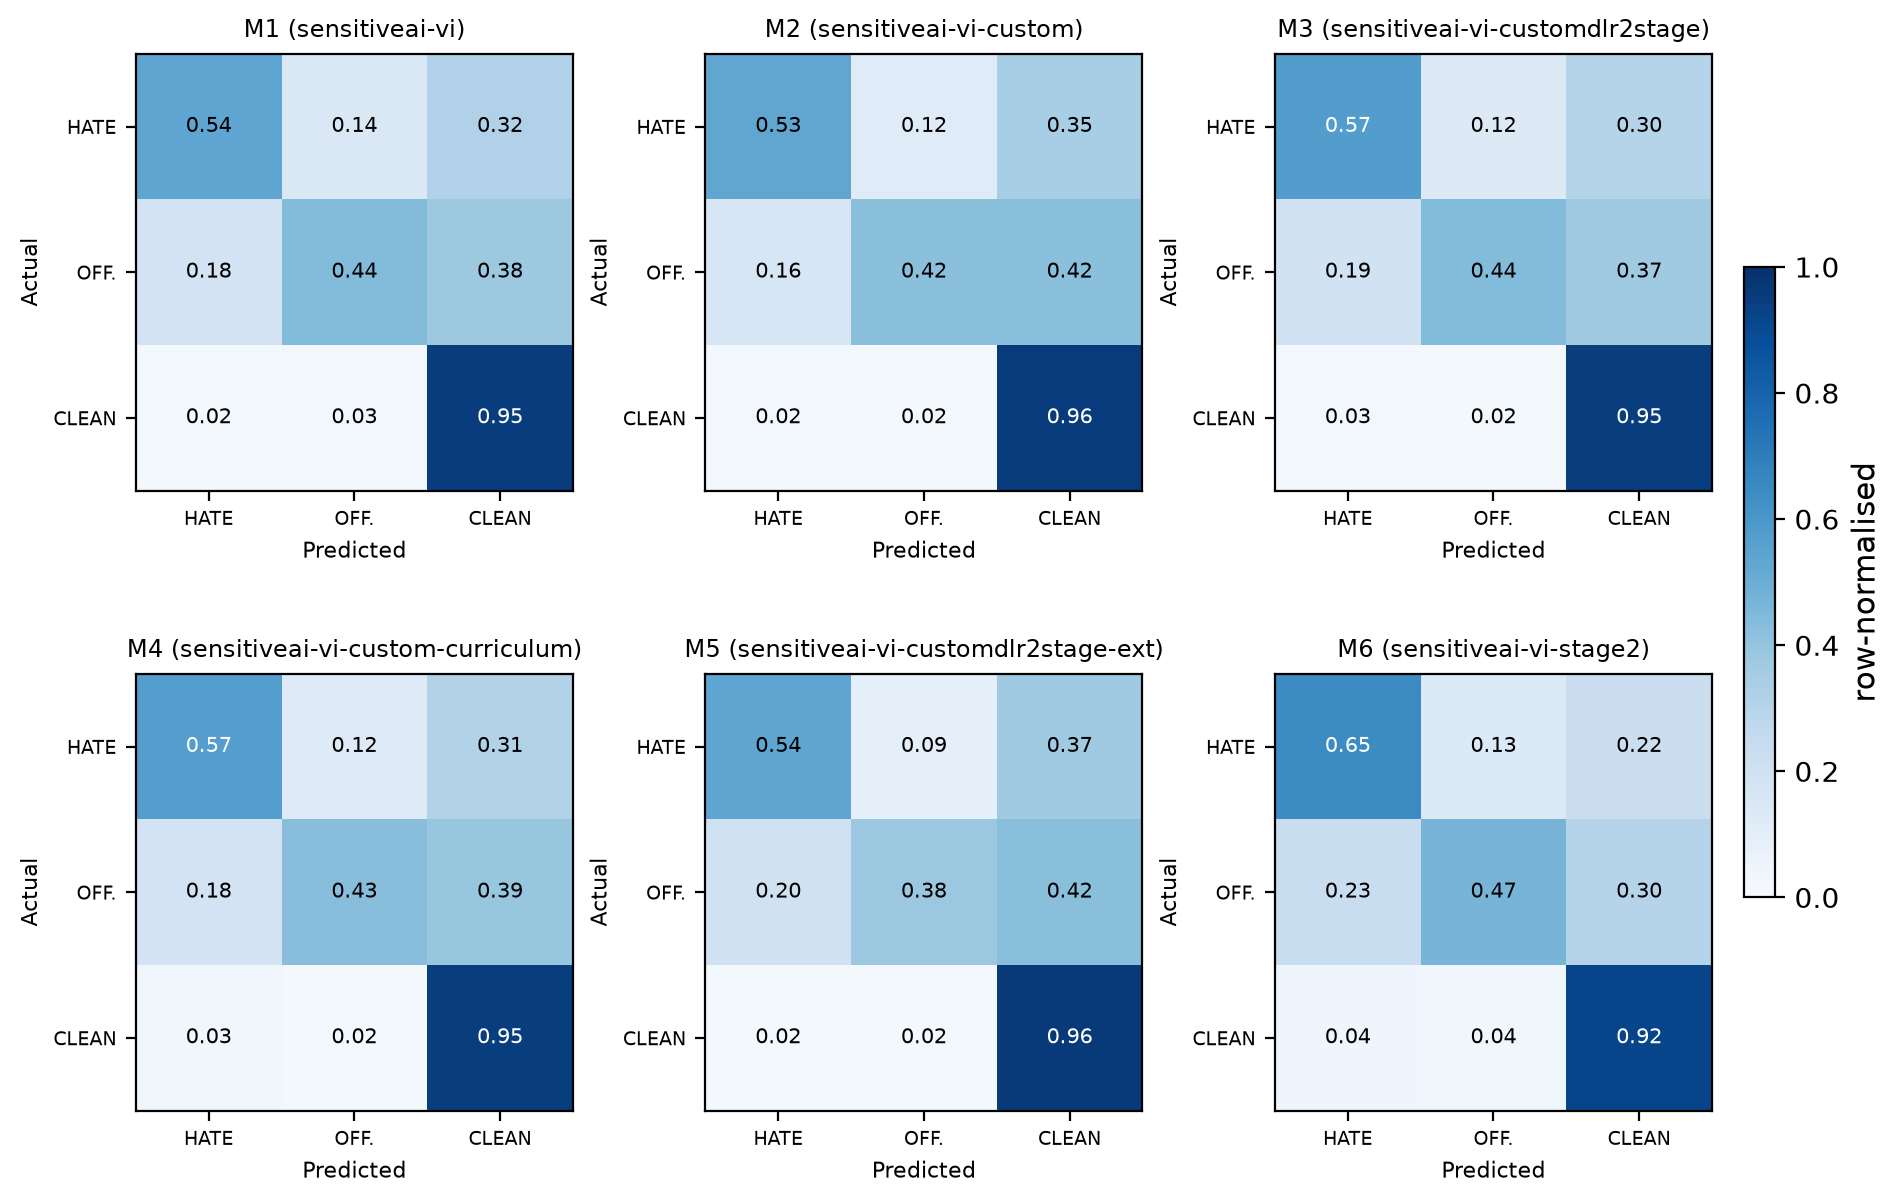
\includegraphics[width=0.98\textwidth]{confusion_grid.png}
\caption{Normalised confusion matrices (rows = true, columns = predicted) for
the six systems, on the same colour scale.  \model{M6} (bottom right) trades
CLEAN recall for minority recall relative to the other five.}
\label{fig:supp-confusion}
\end{figure}

\section{Ranking Quality: ROC-AUC, Average Precision and MCC}
\label{sec:supp-ranking}

Accuracy and macro-F1 depend on a decision rule; the one-vs-rest ranking
metrics do not, and so they separate ``the model ranks the classes well'' from
``the threshold happened to be good.''  Table~\ref{tab:supp-ranking} reports
per-class ROC-AUC and average precision (AP)~\cite{saito2015precision}, their
macro and micro averages, and the Matthews correlation coefficient (MCC).  The headline reading is that
the systems are close but not identical: \model{M6} has the best macro ROC-AUC
(0.8930) while \model{M1} has the best macro AP (0.6599), so the best
\emph{ranking of the rare positives} and the best \emph{recall of the rare
positives} do not belong to the same recipe.  MCC, which is insensitive to the
CLEAN majority, is highest for \model{M3} (0.5650), agreeing with its best
macro-F1.

% AUTO-GENERATED by scripts/11_supplementary_analyses.py - do not edit by hand.
\begin{table}[!htbp]
\centering
\footnotesize
\setlength{\tabcolsep}{3pt}
\caption{One-vs-rest ranking quality per class (ROC-AUC / average precision) and the macro averages, for all six systems.  Best macro value in bold.}
\label{tab:supp-ranking}
\begin{tabular}{lcccccc}
\toprule
 & \multicolumn{2}{c}{HATE} & \multicolumn{2}{c}{OFFENSIVE} & \multicolumn{2}{c}{CLEAN} \\
\cmidrule(lr){2-3} \cmidrule(lr){4-5} \cmidrule(lr){6-7}
System & AUC & AP & AUC & AP & AUC & AP \\
\midrule
M1 & 0.8946 & 0.5982 & 0.8686 & 0.4119 & 0.8987 & 0.9698 \\
M2 & 0.8966 & 0.5717 & 0.8635 & 0.4052 & 0.8924 & 0.9684 \\
M3 & 0.8538 & 0.5354 & 0.8532 & 0.3898 & 0.8713 & 0.9511 \\
M4 & 0.8799 & 0.5735 & 0.8002 & 0.3844 & 0.8700 & 0.9522 \\
M5 & 0.9100 & 0.5707 & 0.7221 & 0.3625 & 0.7967 & 0.9042 \\
M6 & 0.8985 & 0.5688 & 0.8724 & 0.4182 & 0.9079 & 0.9731 \\
\midrule
System & \multicolumn{2}{c}{macro AUC / AP} & \multicolumn{2}{c}{micro AUC / AP} & \multicolumn{2}{c}{MCC} \\
\midrule
M1 & \multicolumn{2}{c}{0.8873 / \textbf{0.6599}} & \multicolumn{2}{c}{0.9635 / 0.9361} & \multicolumn{2}{c}{0.5541} \\
M2 & \multicolumn{2}{c}{0.8842 / 0.6484} & \multicolumn{2}{c}{0.9604 / 0.9332} & \multicolumn{2}{c}{0.5533} \\
M3 & \multicolumn{2}{c}{0.8594 / 0.6254} & \multicolumn{2}{c}{0.9577 / 0.9189} & \multicolumn{2}{c}{0.5650} \\
M4 & \multicolumn{2}{c}{0.8500 / 0.6367} & \multicolumn{2}{c}{0.9528 / 0.9158} & \multicolumn{2}{c}{0.5550} \\
M5 & \multicolumn{2}{c}{0.8096 / 0.6124} & \multicolumn{2}{c}{0.9346 / 0.8481} & \multicolumn{2}{c}{0.5538} \\
M6 & \multicolumn{2}{c}{\textbf{0.8930} / 0.6534} & \multicolumn{2}{c}{0.9575 / 0.9311} & \multicolumn{2}{c}{0.5636} \\
\bottomrule
\end{tabular}
\end{table}


The per-class ROC and precision--recall curves for all six systems are reproduced
in Sect.~\ref{sec:supp-comparison-figures}; this table is their numerical
companion.

\section{Posterior Calibration}
\label{sec:supp-calibration}

A system can be accurate yet over-confident, which matters when its scores are
used as moderation signals.  Table~\ref{tab:supp-calibration} therefore reports
top-label expected calibration error (ECE, 10 equal-width bins), the multiclass
Brier score and the negative log-likelihood (NLL) of the frozen posteriors, all
computed on the test set.  \model{M6} is the best-calibrated system on every
metric (ECE $0.068$, Brier $0.217$, NLL $0.482$), with a mean confidence of
$0.931$; the class-weighted cross-entropy systems (\model{M3}, \model{M5}) are the
most over-confident (mean confidence $0.996$) and have the worst NLL
($>1.0$), i.e.\ they are frequently very confident and wrong.  The reliability
diagram is shown in Fig.~\ref{fig:supp-reliability}.

% AUTO-GENERATED by scripts/11_supplementary_analyses.py - do not edit by hand.
\begin{table}[!htbp]
\centering
\footnotesize
\setlength{\tabcolsep}{4pt}
\caption{Calibration of the frozen posteriors on the test set: top-label expected calibration error (ECE, 10 bins), multiclass Brier score and negative log-likelihood (lower is better).  Best per column in bold.}
\label{tab:supp-calibration}
\begin{tabular}{lcccc}
\toprule
System & ECE $\downarrow$ & Brier $\downarrow$ & NLL $\downarrow$ & mean conf. \\
\midrule
M1 & 0.106 & 0.228 & 0.622 & 0.979 \\
M2 & 0.111 & 0.233 & 0.838 & 0.987 \\
M3 & 0.120 & 0.244 & 1.191 & 0.996 \\
M4 & 0.119 & 0.241 & 1.044 & 0.993 \\
M5 & 0.118 & 0.237 & 1.047 & 0.996 \\
M6 & \textbf{0.068} & \textbf{0.217} & \textbf{0.482} & 0.931 \\
\bottomrule
\end{tabular}
\end{table}


\begin{figure}[!htbp]
\centering
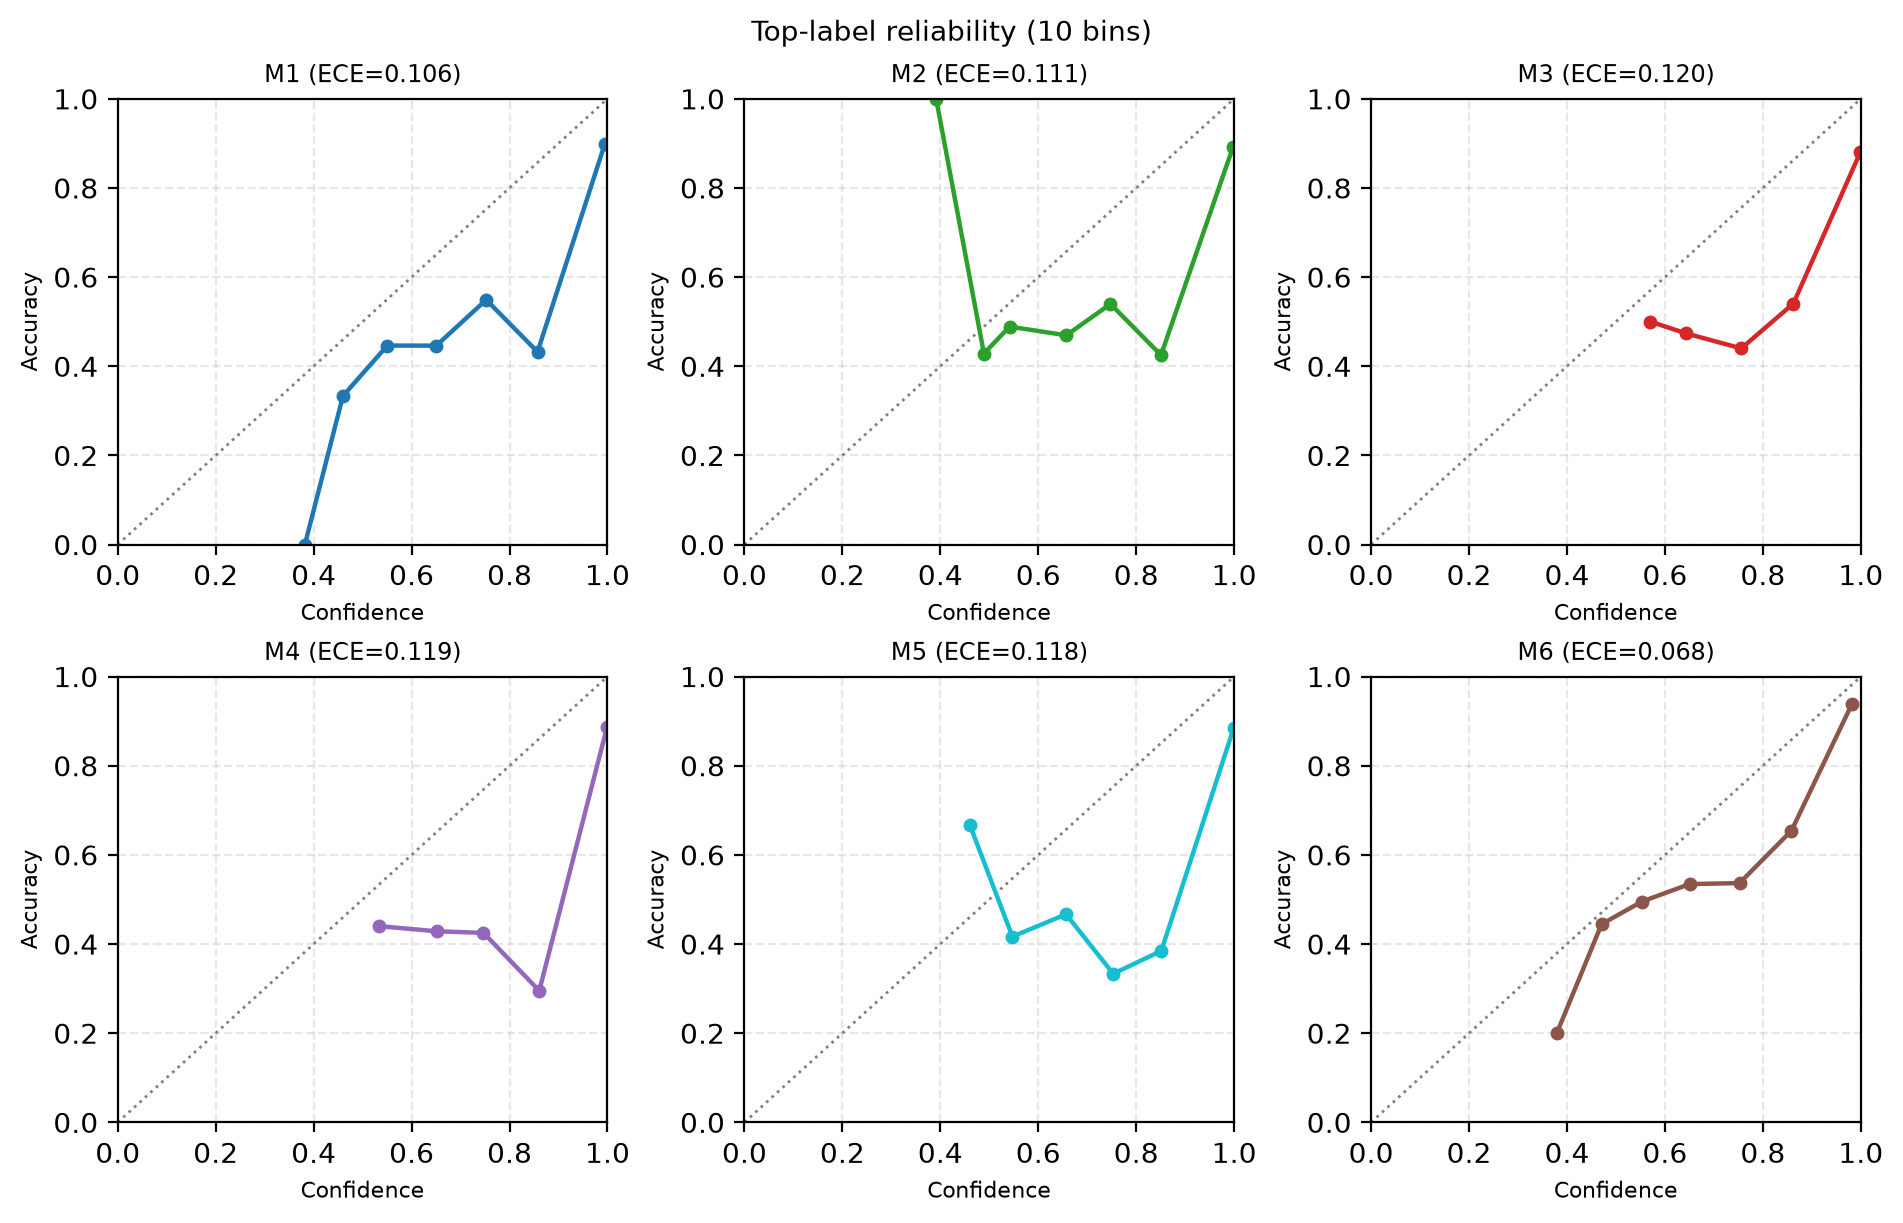
\includegraphics[width=0.62\textwidth]{reliability.png}
\caption{Reliability diagram of the top-label confidence for the six systems
(10 bins).  The dashed diagonal is perfect calibration.  \model{M6} sits closest
to the diagonal; \model{M3} and \model{M5} are the most over-confident.}
\label{fig:supp-reliability}
\end{figure}

\section{Error Complementarity}
\label{sec:supp-error}

\emph{Do the systems make the same mistakes, or different ones?}  For each test
comment we count how many of the six systems misclassify it.
Table~\ref{tab:supp-error-overlap} (top) gives the distribution over
$k = 0,\dots,6$: 5{,}410 comments are solved by all six and 504 (7.5\% of the
test set) are missed by all six, with the remaining 766 split across the middle
bins.  The 504 all-miss comments are the hard core (HATE 185, OFFENSIVE 180,
CLEAN 139) and set a floor that no recipe in this family reaches past.
Fig.~\ref{fig:supp-error-overlap} visualises the same distribution.

% AUTO-GENERATED by scripts/11_supplementary_analyses.py - do not edit by hand.
\begin{table}[!htbp]
\centering
\footnotesize
\setlength{\tabcolsep}{4pt}
\caption{Error complementarity across the six systems.  \emph{Top:} how many test comments are misclassified by exactly $k$ systems.  \emph{Bottom:} the comments no system gets right, broken down by their gold label.}
\label{tab:supp-error-overlap}
\begin{tabular}{lccccccc}
\toprule
\# systems wrong & 0 & 1 & 2 & 3 & 4 & 5 & 6 \\
\midrule
test comments & 5,410 & 228 & 178 & 93 & 143 & 124 & 504 \\
\midrule
\multicolumn{8}{l}{\emph{missed by all six:} 504 comments (HATE 185, OFFENSIVE 180, CLEAN 139)} \\
\multicolumn{8}{l}{\emph{solved by all six:} 5410 comments (HATE 270, OFFENSIVE 130, CLEAN 5010)} \\
\bottomrule
\end{tabular}
\end{table}


\begin{figure}[!htbp]
\centering
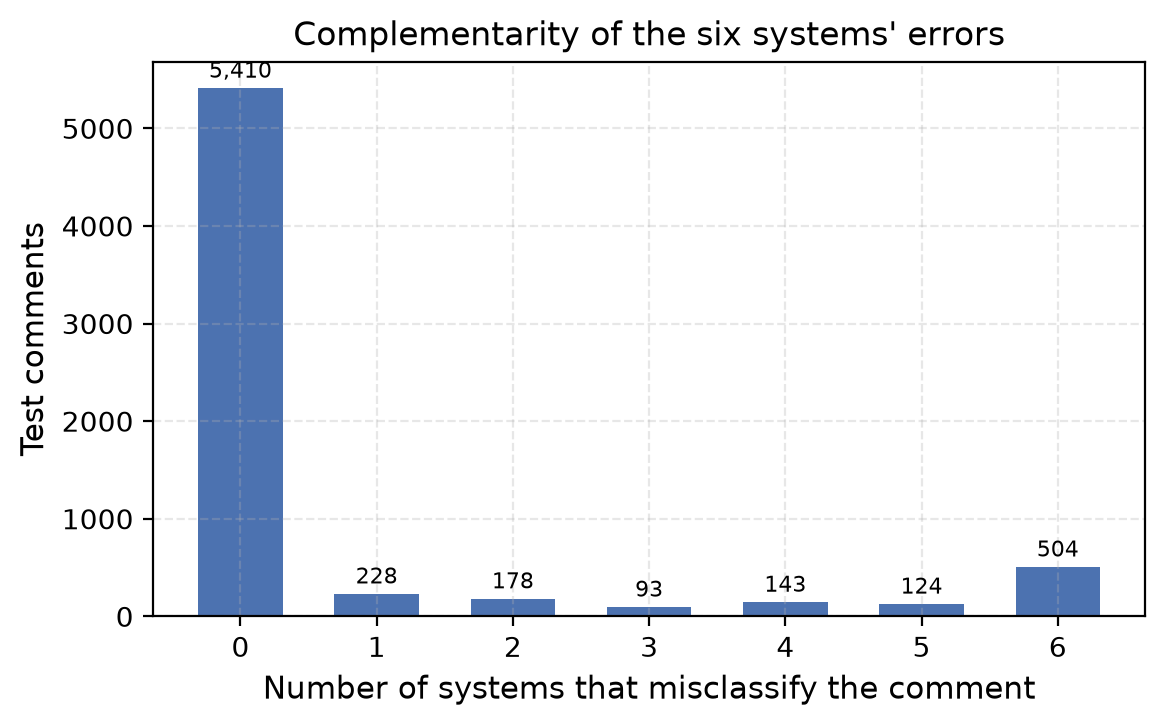
\includegraphics[width=0.7\textwidth]{error_overlap.png}
\caption{Number of test comments misclassified by exactly $k$ of the six
systems.  The spike at $k=6$ is the 504-comment hard core; the rest is spread
thinly, i.e.\ the systems mostly agree on which items are easy.}
\label{fig:supp-error-overlap}
\end{figure}

Table~\ref{tab:supp-unique-errors} isolates the opposite quantity: errors made
by \emph{exactly one} system.  \model{M6} has 109 unique errors, an order of
magnitude more than \model{M3} (11) or \model{M2} (25); its errors are both the
most numerous (913) and the least shared with the other systems, which is the
error-profile counterpart of its minority-recall-heavy operating point.

% AUTO-GENERATED by scripts/11_supplementary_analyses.py - do not edit by hand.
\begin{table}[!htbp]
\centering
\footnotesize
\setlength{\tabcolsep}{4pt}
\caption{Errors made by exactly one system (out of the six).  A high count means the system's mistakes are largely its own; a low count means its errors are shared with the others.}
\label{tab:supp-unique-errors}
\begin{tabular}{lrr}
\toprule
System & unique errors & total errors \\
\midrule
M1 & 43 & 846 \\
M2 & 25 & 827 \\
M3 & 11 & 832 \\
M4 & 20 & 848 \\
M5 & 20 & 813 \\
M6 & 109 & 913 \\
\bottomrule
\end{tabular}
\end{table}


\section{Stratified Macro-F1 by Surface Phenomenon}
\label{sec:supp-strata}

Vietnamese social-media text is noisy in ways that are not captured by a single
accuracy number.  Table~\ref{tab:supp-stratification} recomputes macro-F1
within overlapping surface strata (emoji, teencode, repeated characters,
missing/with diacritics, and very short / very long comments) defined by simple
lexical rules on the raw comment.  Strata overlap, so a comment can appear in
several rows.  Two patterns stand out: (i) \emph{very long} comments are the
hardest stratum for every system (macro-F1 $0.52$--$0.61$, $n=145$) and the
largest gap between systems, where \model{M3} leads (0.6118) and \model{M1}
lags (0.5212); (ii) on short comments, which are the majority ($n=1{,}852$ for
\emph{very short}), the six systems fall within 0.015 of one another
($0.698$--$0.713$).  These are descriptive within-stratum gaps on a single test
split; we do not attribute them to a causal effect of any surface phenomenon.

% AUTO-GENERATED by scripts/11_supplementary_analyses.py - do not edit by hand.
\begin{table}[!htbp]
\centering
\footnotesize
\setlength{\tabcolsep}{3pt}
\caption{Macro-F1 by surface phenomenon of the test comments, for all six systems.  Strata overlap (a comment can be both short and teencode); counts are the number of test comments carrying the tag.}
\label{tab:supp-stratification}
\begin{tabular}{lccccccr}
\toprule
Stratum & M1 & M2 & M3 & M4 & M5 & M6 & n \\
\midrule
\texttt{emoji} & 0.5826 & 0.6165 & 0.6417 & 0.6397 & 0.6266 & 0.6522 & 974 \\
\texttt{no\_diacritics} & 0.6120 & 0.6336 & 0.6382 & 0.6191 & 0.6283 & 0.5882 & 370 \\
\texttt{repeat\_chars} & 0.6820 & 0.6988 & 0.6913 & 0.6861 & 0.6783 & 0.6651 & 997 \\
\texttt{teencode} & 0.6527 & 0.6301 & 0.6520 & 0.6480 & 0.6476 & 0.6591 & 1,039 \\
\texttt{very\_long} & 0.5212 & 0.5677 & 0.6118 & 0.6029 & 0.5256 & 0.5411 & 145 \\
\texttt{very\_short} & 0.7098 & 0.7090 & 0.7132 & 0.6981 & 0.7087 & 0.7083 & 1,852 \\
\texttt{with\_diacritics} & 0.6537 & 0.6562 & 0.6628 & 0.6592 & 0.6531 & 0.6627 & 6,114 \\
\bottomrule
\end{tabular}
\end{table}


\section{Comparison Figures Across the Six Systems}
\label{sec:supp-comparison-figures}

The figures below are the full set produced by the evaluation pipeline.  Each
plot compares all six systems on the same axis so that the differences in
accuracy, macro-F1, per-class F1, validation loss and validation accuracy, and
the ranking quality, can be read off directly.  They expand on the summary
tables above; nothing here is tuned on the test set.  Two readings are worth
flagging.  First, the accuracy leader is \model{M5} ($0.878$), not \model{M6}
($0.863$, the lowest); the gap reverses on macro-F1, where \model{M5} is last
($0.654$) and \model{M3} first ($0.664$), which is the accuracy/macro-F1 trap
made visible.  Second, the validation-loss curves are \emph{not} the model
selection criterion: the selected checkpoint is the epoch with the highest
validation macro-F1 (\path{src/callbacks/monitoring.py}), so the frozen epoch
need not be the loss minimum.

% AUTO-GENERATED by scripts/11_supplementary_analyses.py - do not edit by hand.

\begin{figure}[htbp]
\centering
\begin{minipage}{0.74\textwidth}\centering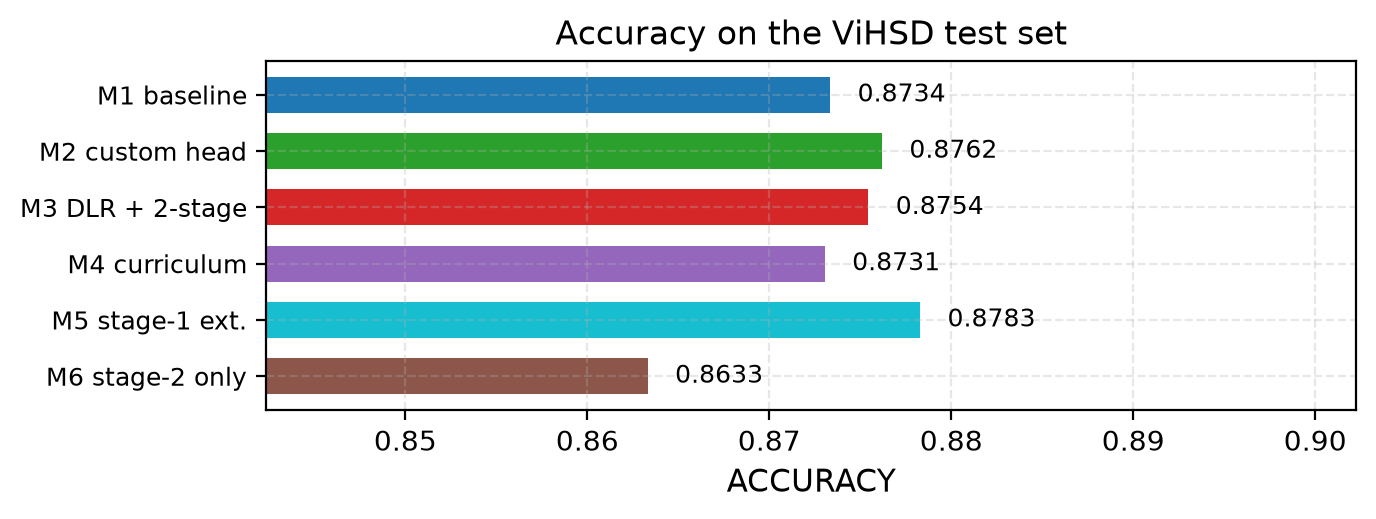
\includegraphics[width=\linewidth]{figures/comparison/accuracy_all_models.png}\caption{\label{fig:supp-acc}Test accuracy for all six systems with 95\% bootstrap confidence intervals.  The highest accuracy belongs to \model{M5}, which does not have the best macro-F1.}\end{minipage}
\end{figure}

\begin{figure}[htbp]
\centering
\begin{minipage}{0.74\textwidth}\centering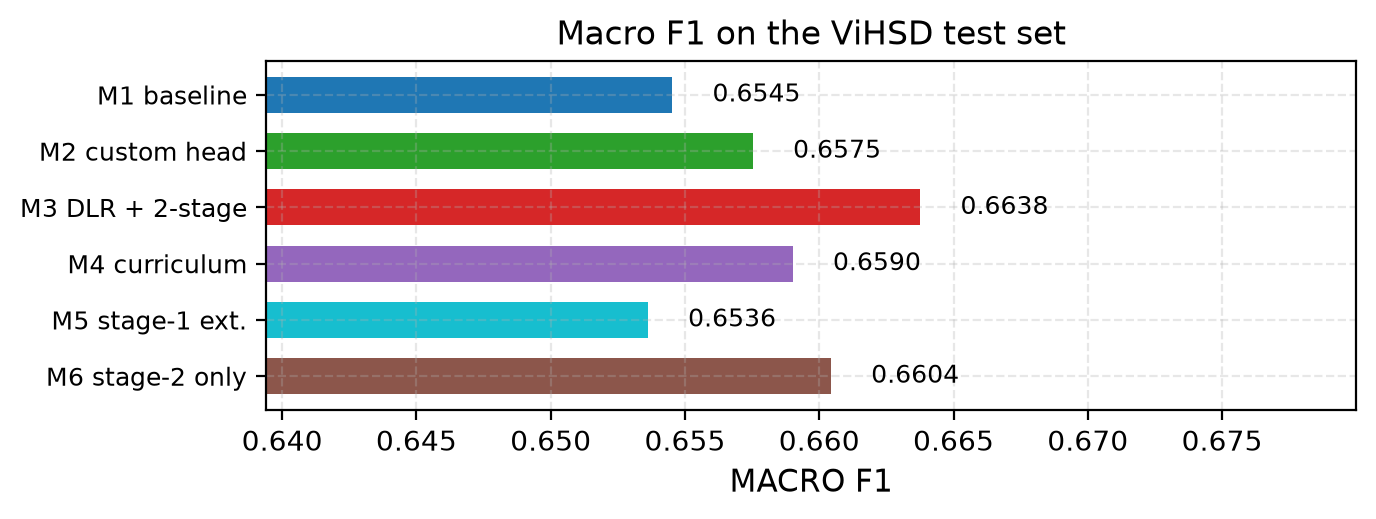
\includegraphics[width=\linewidth]{figures/comparison/macro_f1_all_models.png}\caption{\label{fig:supp-macro-f1}Test macro-F1 (mean of the three class F1 scores) for all six systems.  The six systems sit in a narrow band, which is why no pairwise macro-F1 difference is significant.}\end{minipage}
\end{figure}

\begin{figure}[htbp]
\centering
\begin{minipage}{0.74\textwidth}\centering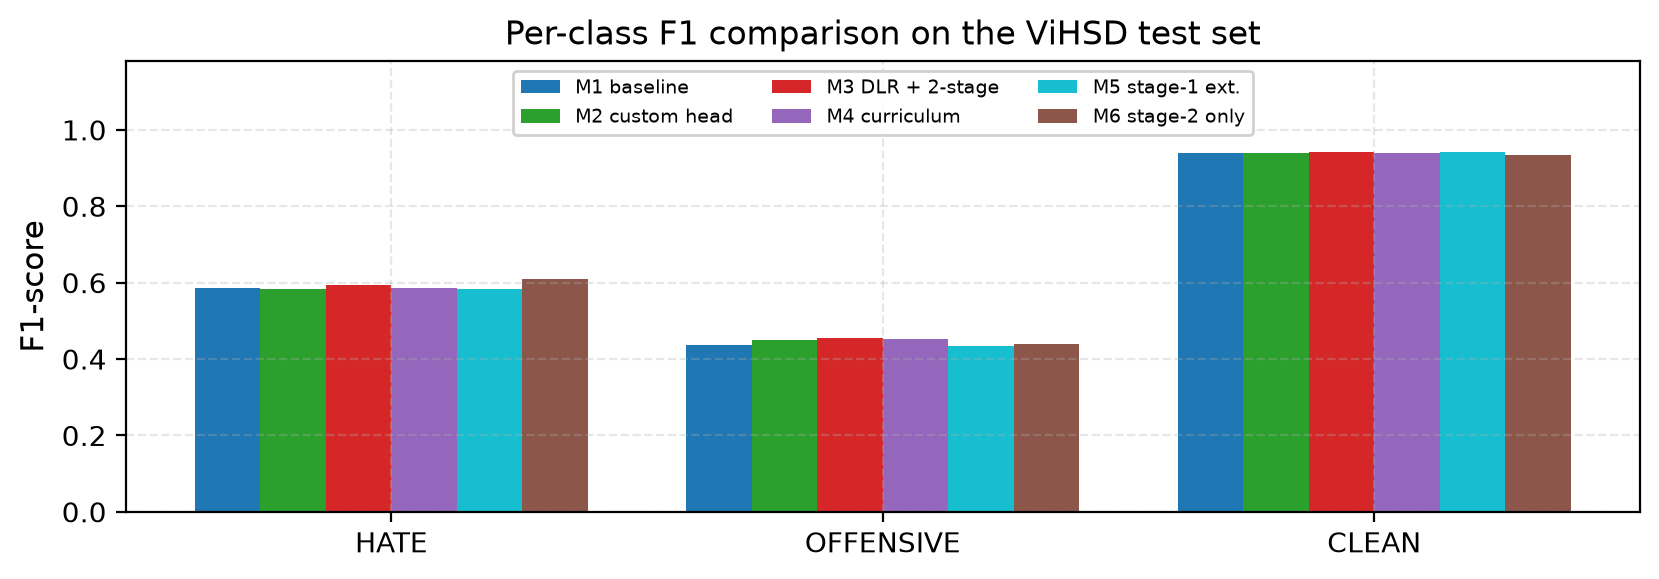
\includegraphics[width=\linewidth]{figures/comparison/per_class_f1_all_models.png}\caption{\label{fig:supp-per-class-f1}Per-class F1 for HATE, OFFENSIVE and CLEAN, grouped by system.  The minority classes (HATE, OFFENSIVE) show the largest spread across systems, while CLEAN is saturated.}\end{minipage}
\end{figure}

\begin{figure}[htbp]
\centering
\begin{minipage}{0.74\textwidth}\centering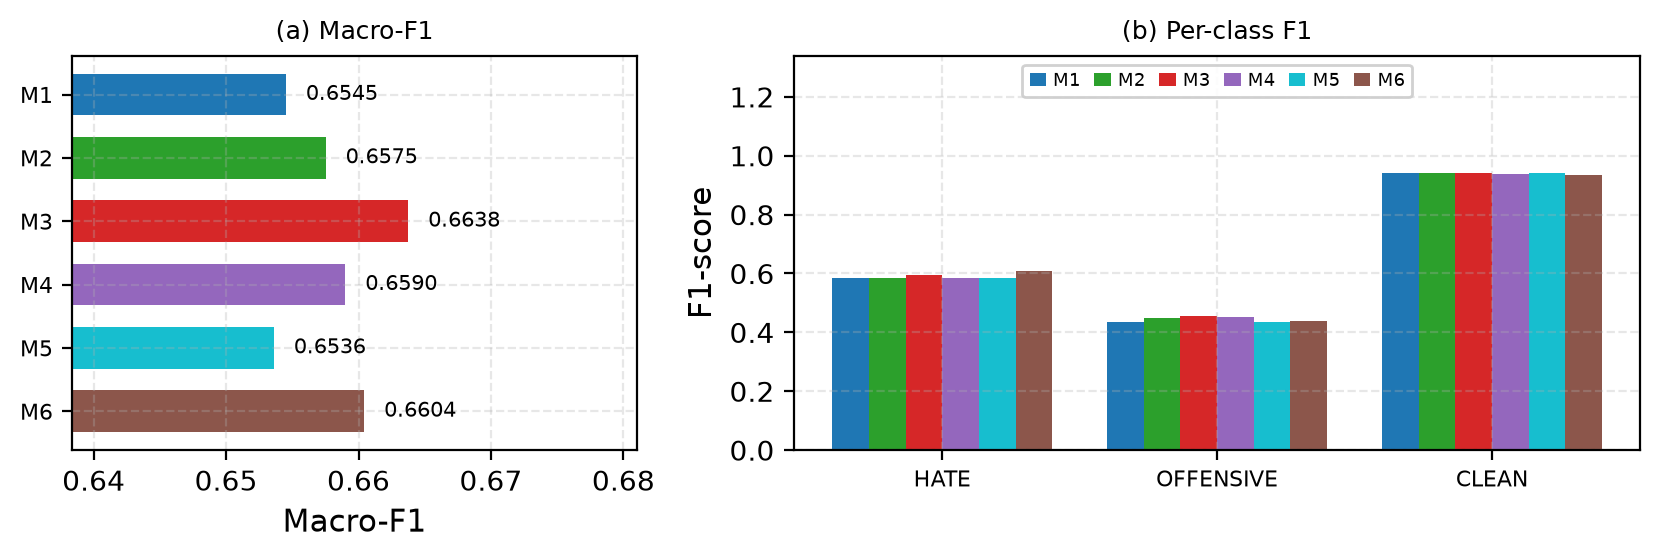
\includegraphics[width=\linewidth]{figures/comparison/f1_summary_all_models.png}\caption{\label{fig:supp-f1-summary}Macro-F1, weighted-F1 and per-class F1 side by side for every system.}\end{minipage}
\end{figure}

\begin{figure}[htbp]
\centering
\begin{minipage}{0.74\textwidth}\centering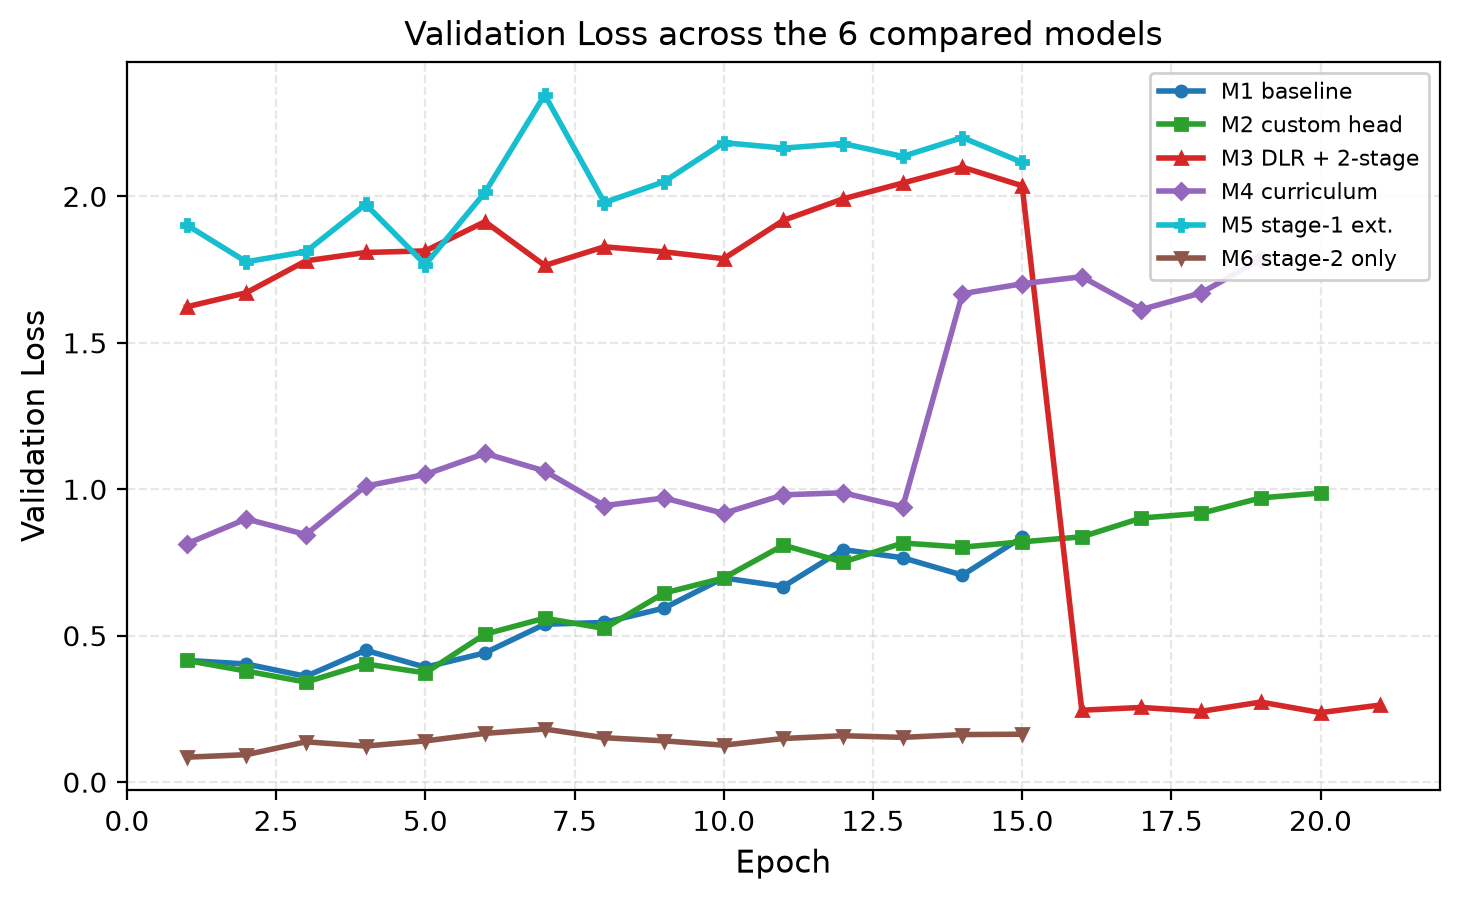
\includegraphics[width=\linewidth]{figures/comparison/validation_loss_all_models.png}\caption{\label{fig:supp-val-loss}Validation loss over the training epochs for all six systems.  The checkpoint is \emph{not} selected to minimise this curve: it is the epoch with the highest validation macro-F1 (Fig.~
ef{fig:supp-val-acc}), which is why the selected checkpoints can sit on a rising-loss epoch.}\end{minipage}
\end{figure}

\begin{figure}[htbp]
\centering
\begin{minipage}{0.74\textwidth}\centering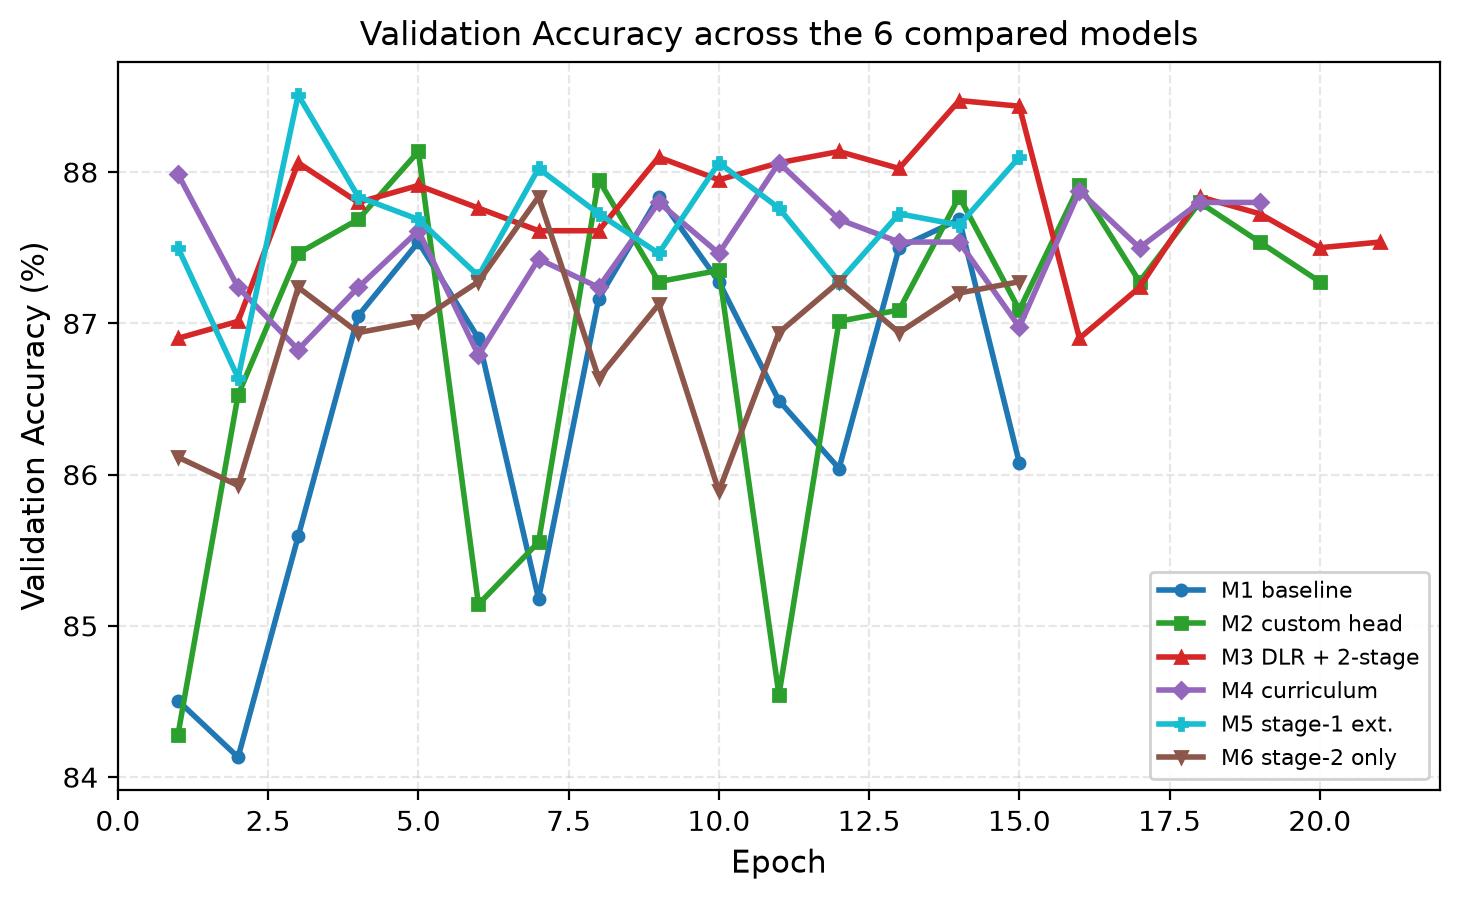
\includegraphics[width=\linewidth]{figures/comparison/validation_accuracy_all_models.png}\caption{\label{fig:supp-val-acc}Validation accuracy over the training epochs for all six systems.}\end{minipage}
\end{figure}

\begin{figure}[htbp]
\centering
\begin{minipage}{0.74\textwidth}\centering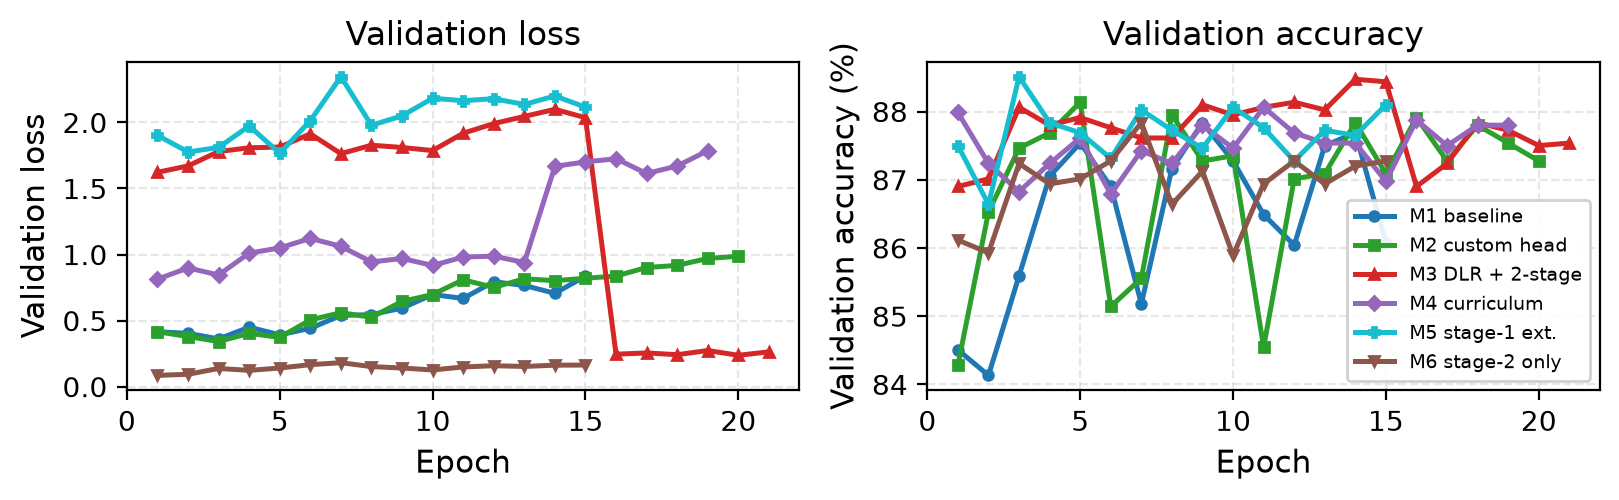
\includegraphics[width=\linewidth]{figures/comparison/validation_loss_accuracy_all_models.png}\caption{\label{fig:supp-val-loss-acc}Validation loss and accuracy on the same axes for all six systems.}\end{minipage}
\end{figure}

\begin{figure}[htbp]
\centering
\begin{minipage}{0.74\textwidth}\centering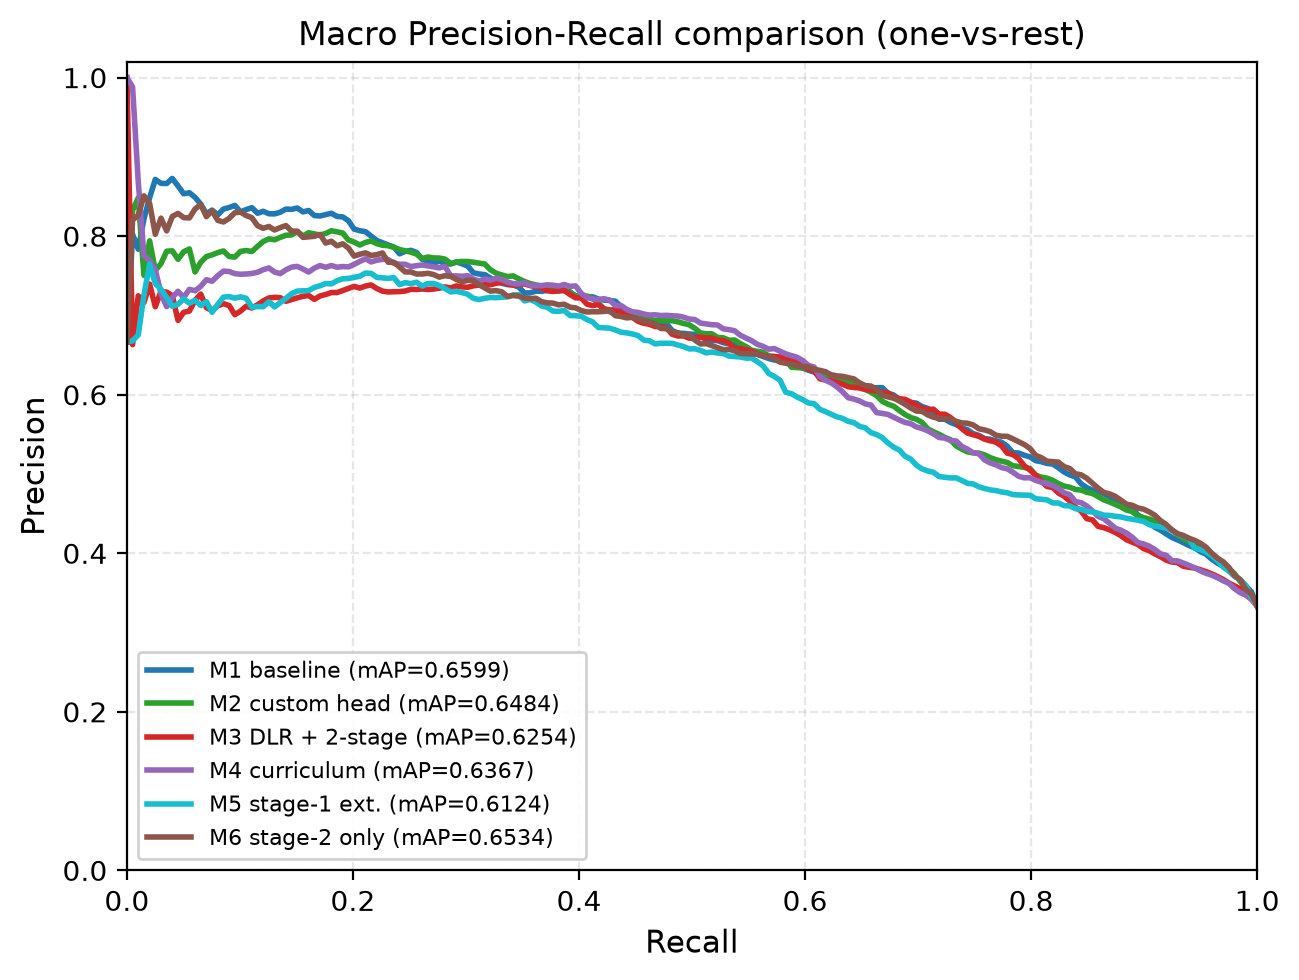
\includegraphics[width=\linewidth]{figures/comparison/pr_curve_all_models.png}\caption{\label{fig:supp-pr-all}One-vs-rest precision--recall curves (micro and macro averages) for all six systems.}\end{minipage}
\end{figure}

\begin{figure}[htbp]
\centering
\begin{minipage}{0.74\textwidth}\centering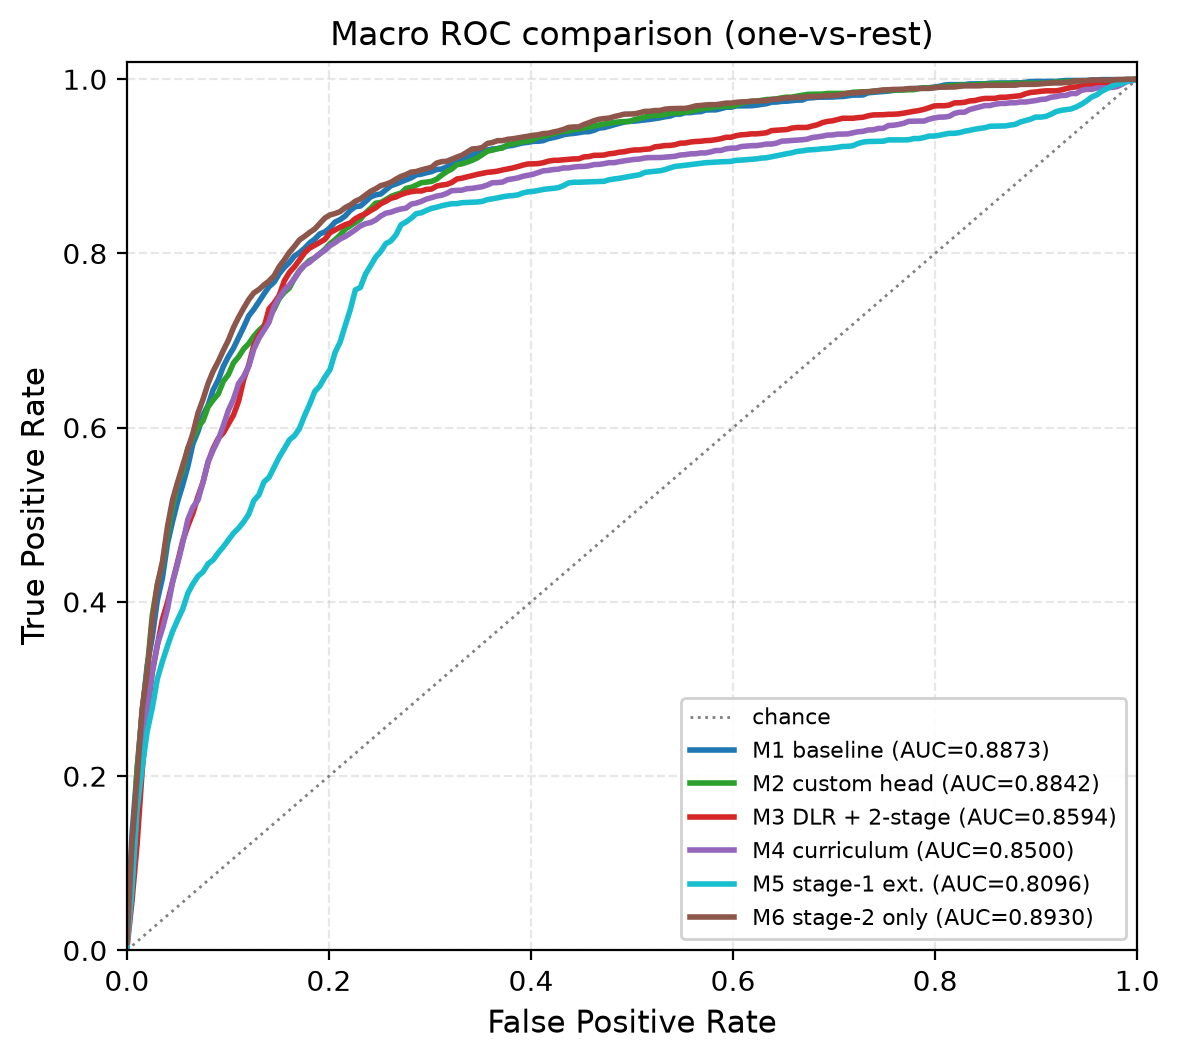
\includegraphics[width=\linewidth]{figures/comparison/roc_curve_all_models.png}\caption{\label{fig:supp-roc-all}One-vs-rest ROC curves (micro and macro averages) for all six systems.}\end{minipage}
\end{figure}

\begin{figure}[htbp]
\centering
\begin{minipage}{0.74\textwidth}\centering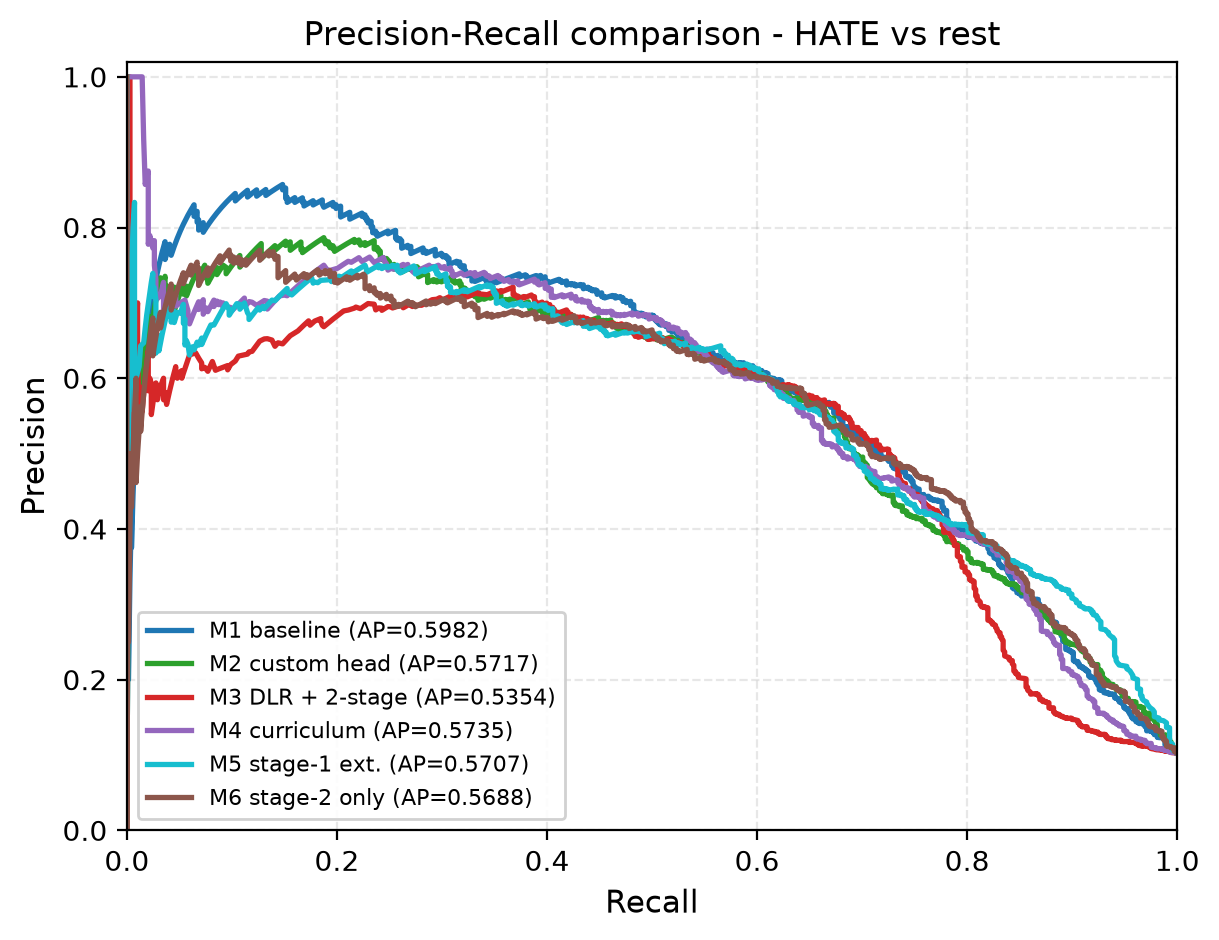
\includegraphics[width=\linewidth]{figures/comparison/pr_hate_all_models.png}\caption{\label{fig:supp-pr-hate}Precision--recall curve for the HATE class, all six systems.}\end{minipage}
\end{figure}

\begin{figure}[htbp]
\centering
\begin{minipage}{0.74\textwidth}\centering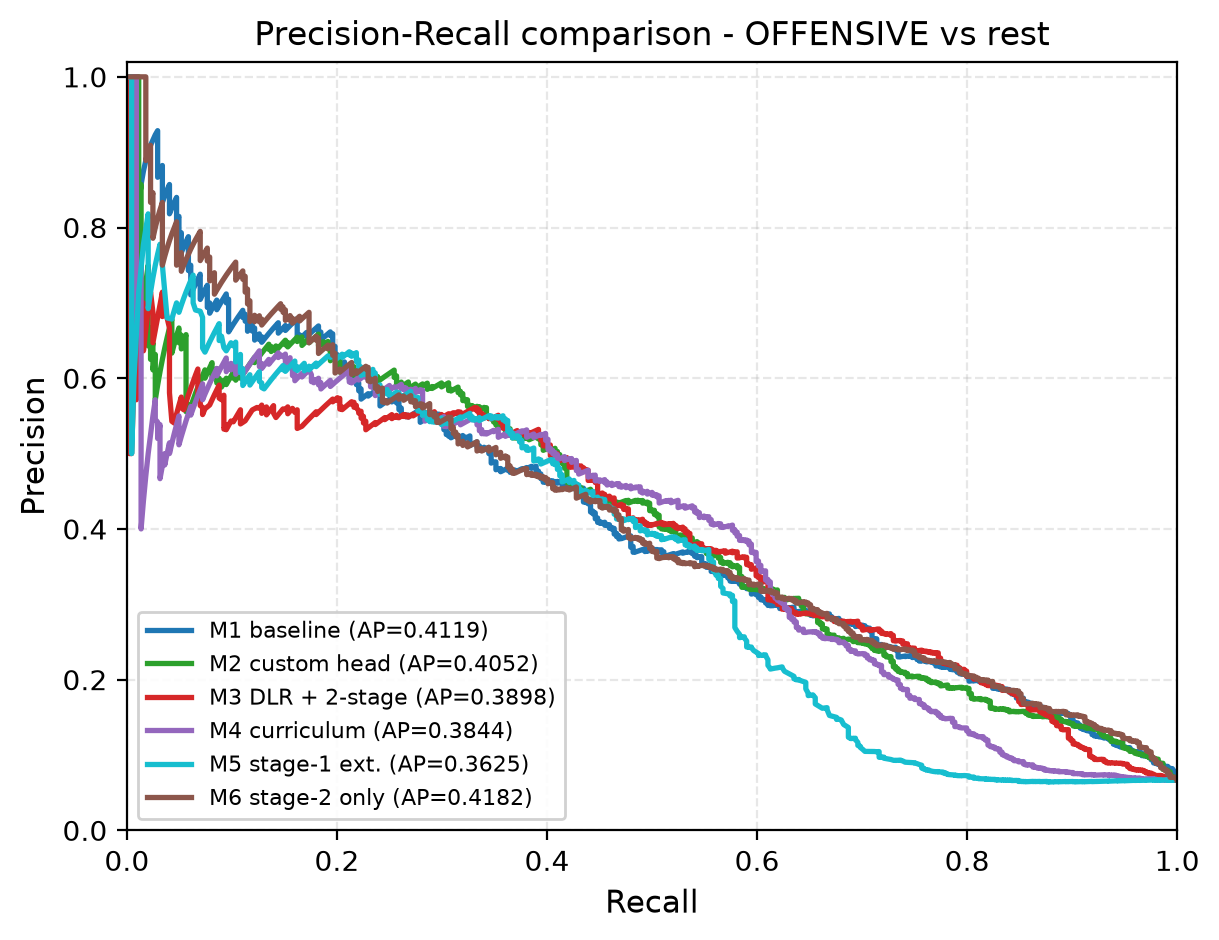
\includegraphics[width=\linewidth]{figures/comparison/pr_offensive_all_models.png}\caption{\label{fig:supp-pr-offensive}Precision--recall curve for the OFFENSIVE class, all six systems.}\end{minipage}
\end{figure}

\begin{figure}[htbp]
\centering
\begin{minipage}{0.74\textwidth}\centering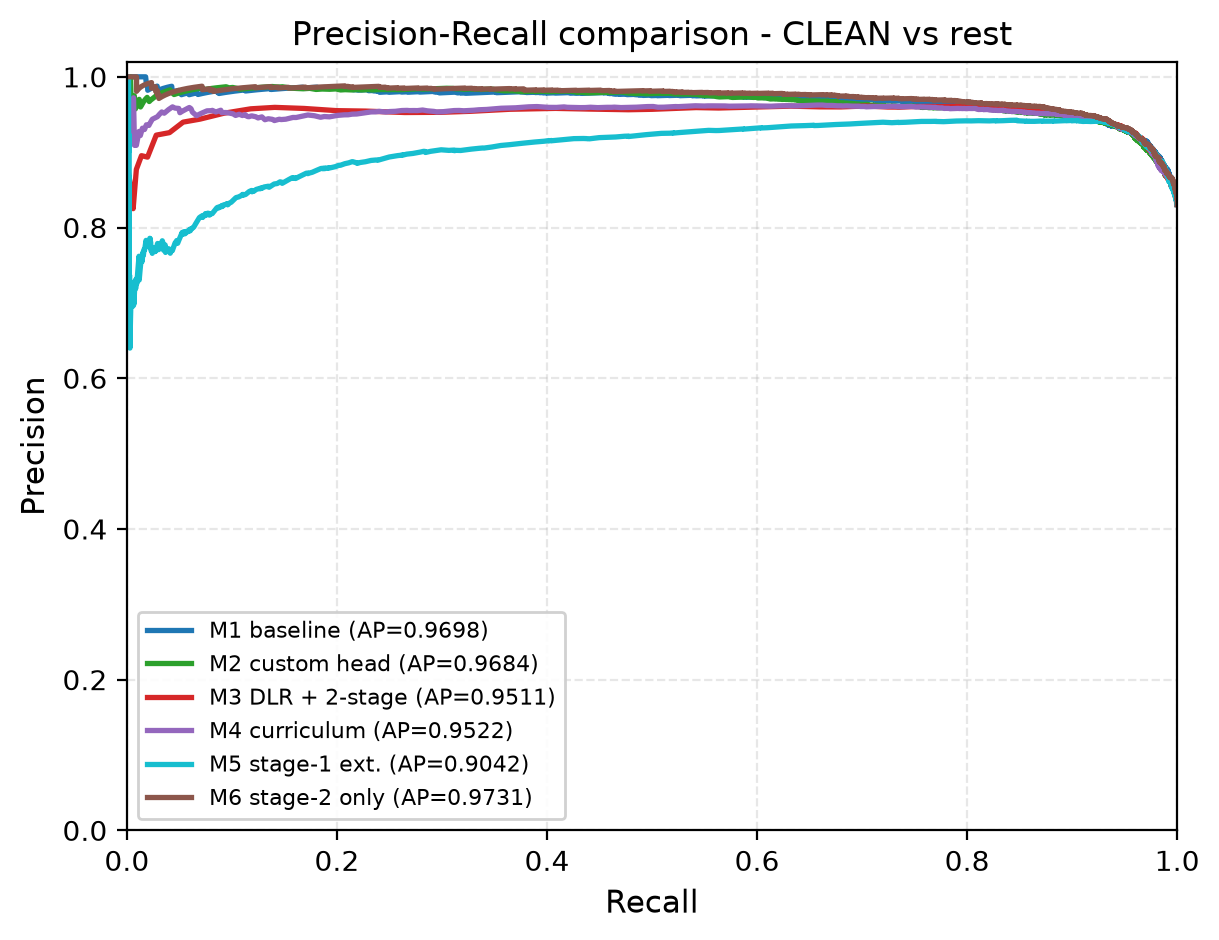
\includegraphics[width=\linewidth]{figures/comparison/pr_clean_all_models.png}\caption{\label{fig:supp-pr-clean}Precision--recall curve for the CLEAN class, all six systems.}\end{minipage}
\end{figure}

\begin{figure}[htbp]
\centering
\begin{minipage}{0.74\textwidth}\centering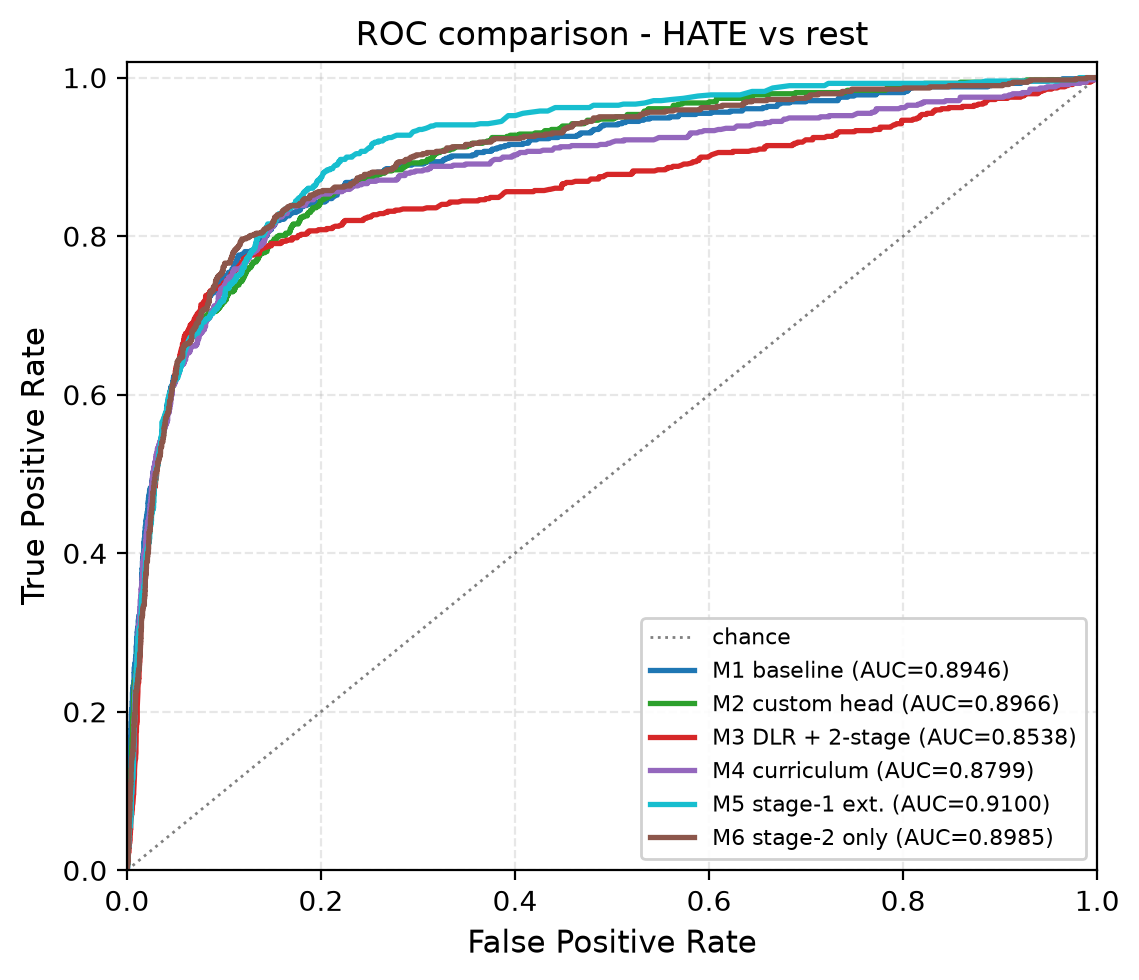
\includegraphics[width=\linewidth]{figures/comparison/roc_hate_all_models.png}\caption{\label{fig:supp-roc-hate}ROC curve for the HATE class, all six systems.}\end{minipage}
\end{figure}

\begin{figure}[htbp]
\centering
\begin{minipage}{0.74\textwidth}\centering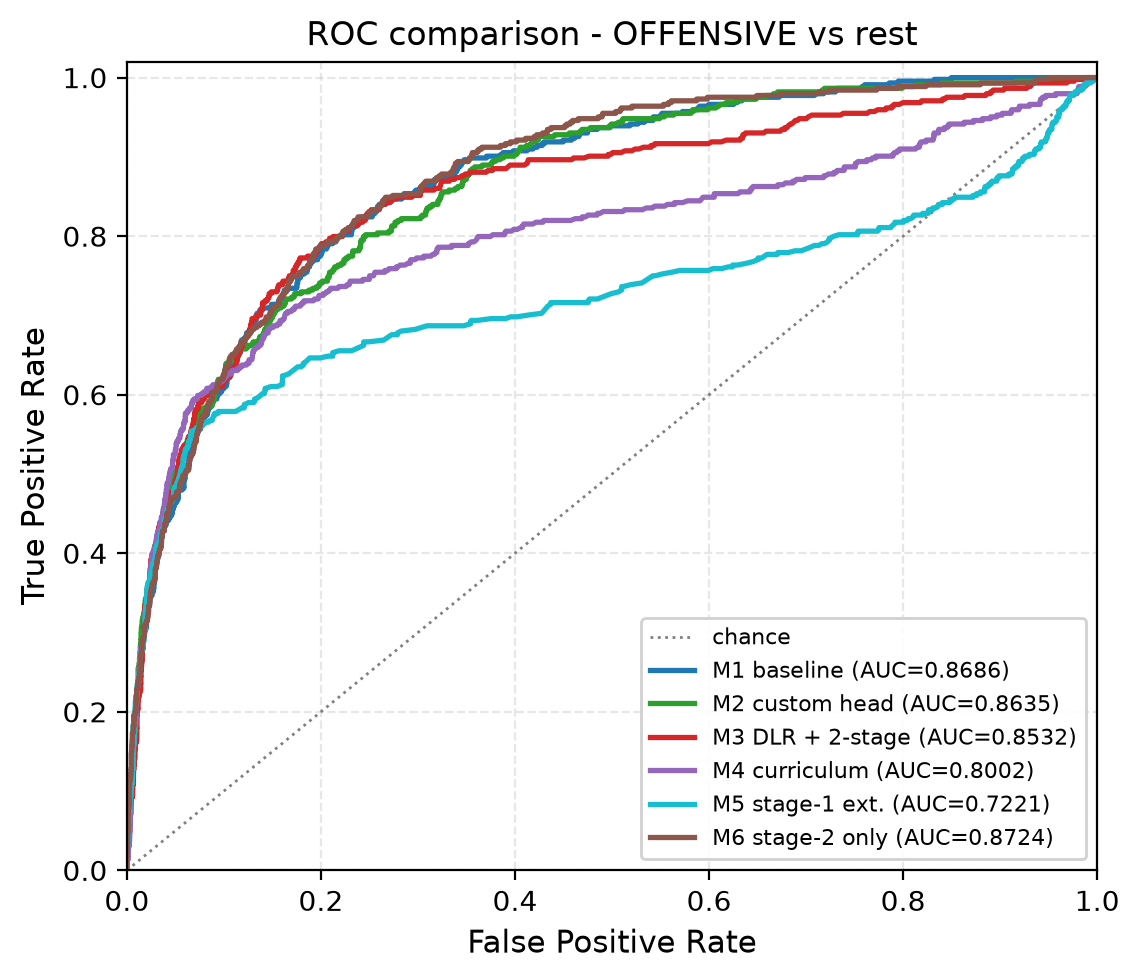
\includegraphics[width=\linewidth]{figures/comparison/roc_offensive_all_models.png}\caption{\label{fig:supp-roc-offensive}ROC curve for the OFFENSIVE class, all six systems.}\end{minipage}
\end{figure}

\begin{figure}[htbp]
\centering
\begin{minipage}{0.74\textwidth}\centering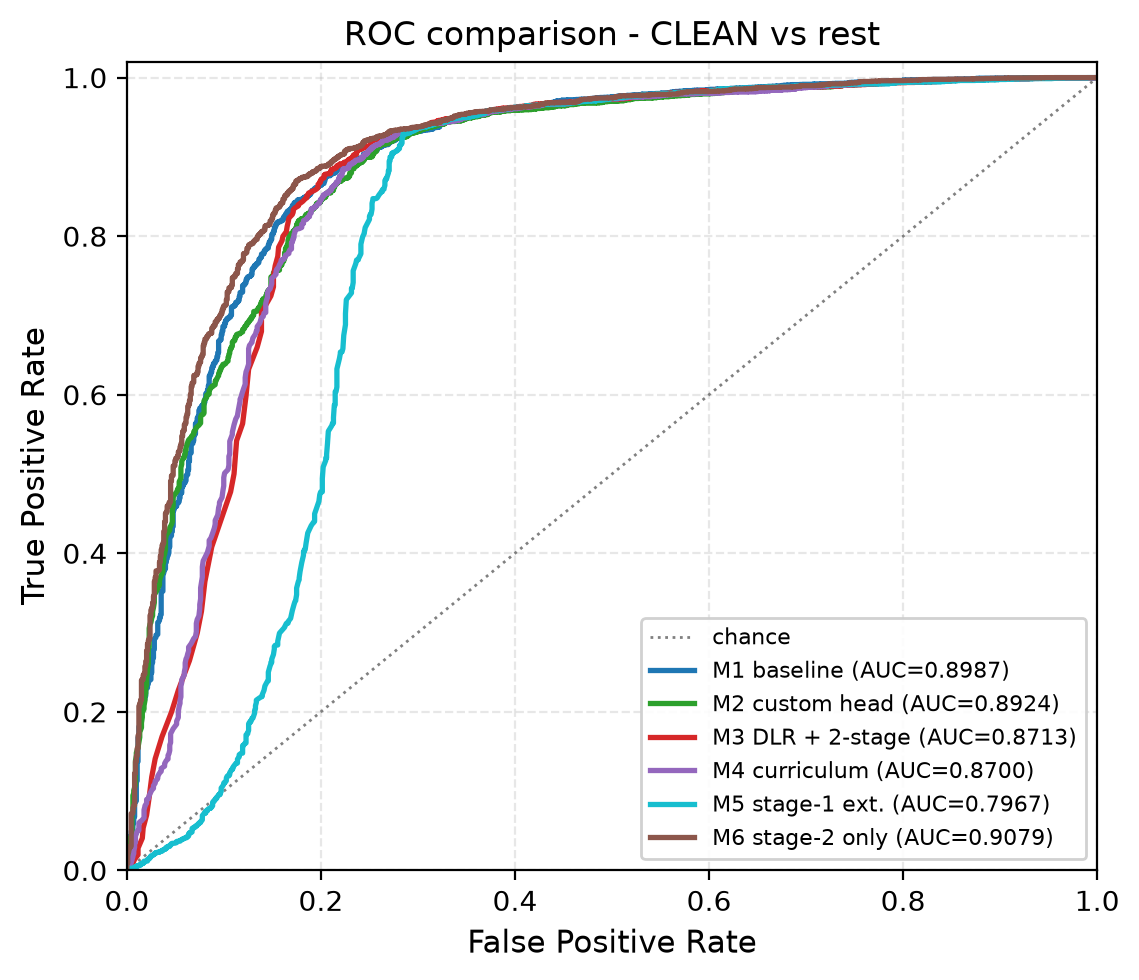
\includegraphics[width=\linewidth]{figures/comparison/roc_clean_all_models.png}\caption{\label{fig:supp-roc-clean}ROC curve for the CLEAN class, all six systems.}\end{minipage}
\end{figure}

\FloatBarrier


\section{Per-System Figures}
\label{sec:supp-per-system-figures}

For each system we reproduce its normalised confusion matrix, its
precision--recall and ROC curves, and its validation loss and accuracy curves.
These are the raw diagnostic plots for every run, laid out one system at a
time so that a reviewer can inspect an individual recipe in isolation.

% AUTO-GENERATED by scripts/11_supplementary_analyses.py - do not edit by hand.

\subsection{\model{M1}}
\label{sec:supp-per-m1}
Baseline: the pre-trained encoder with a standard [CLS] softmax head, single-stage training and plain cross-entropy.  It has the second-best macro average precision (0.6599).

\begin{figure}[htbp]
\centering
\begin{minipage}{0.74\textwidth}\centering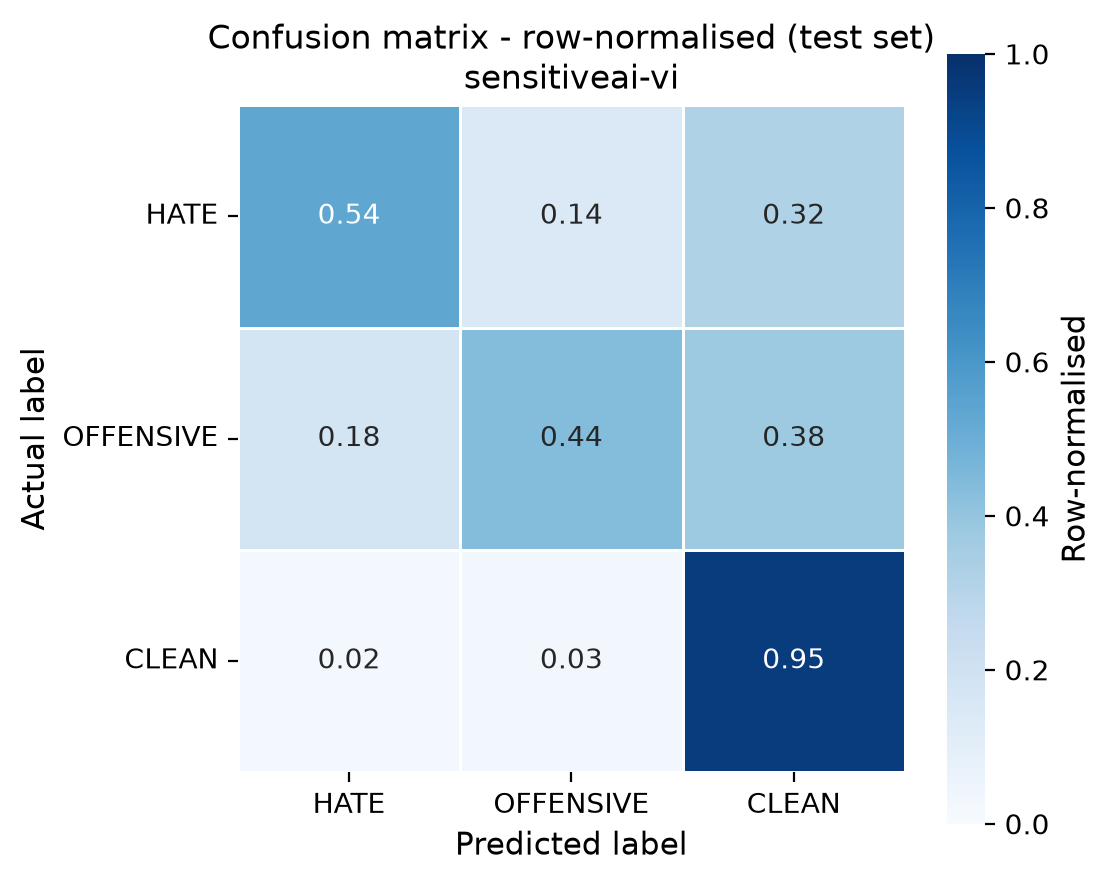
\includegraphics[width=\linewidth]{figures/per_model/M1/confusion_matrix_normalized.png}\caption{Normalised confusion matrix (rows = true, columns = predicted).}\end{minipage}
\end{figure}

\begin{figure}[htbp]
\centering
\begin{minipage}{0.74\textwidth}\centering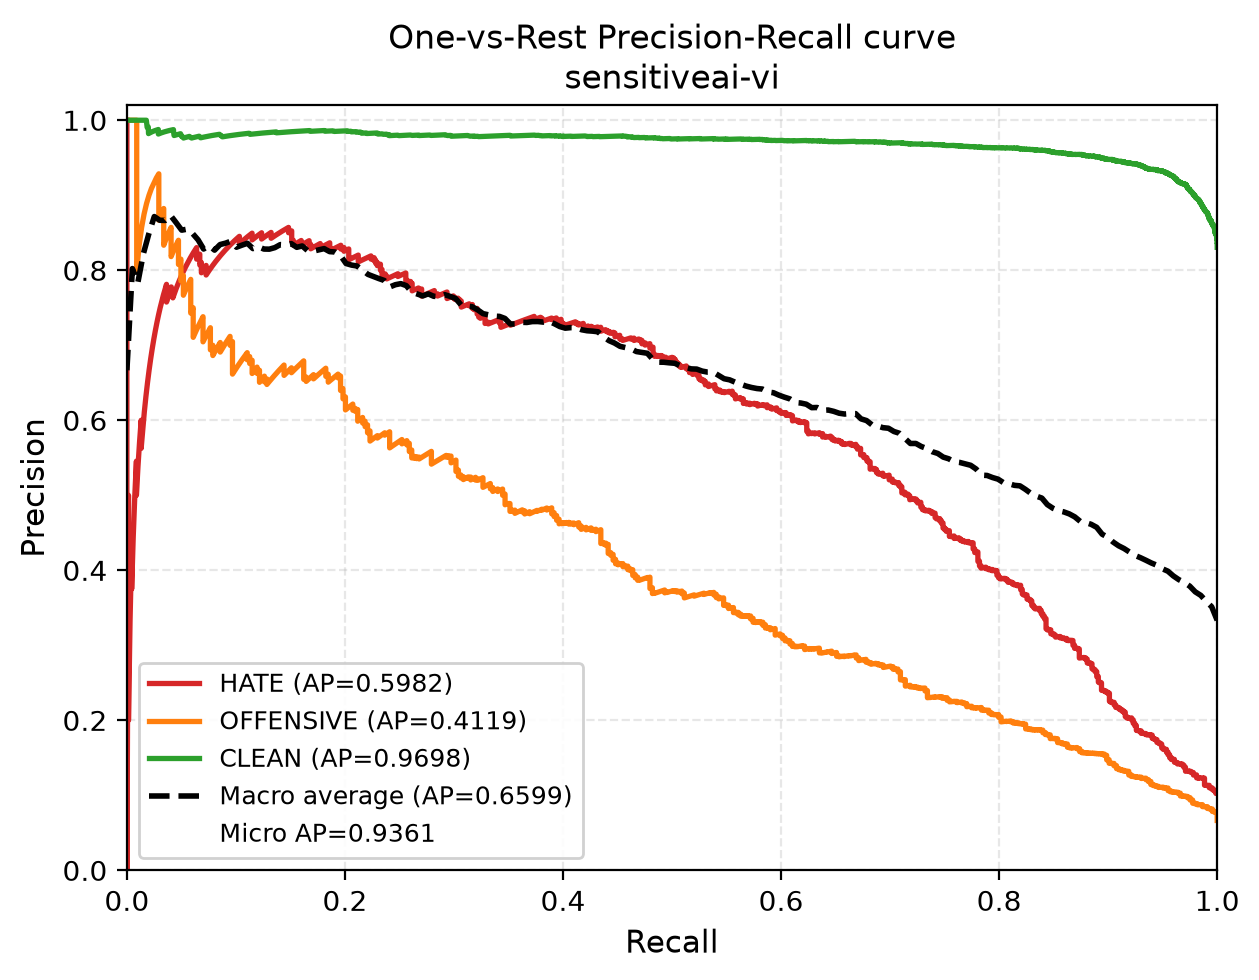
\includegraphics[width=\linewidth]{figures/per_model/M1/pr_curve.png}\caption{Precision--recall curve.}\end{minipage}
\end{figure}

\begin{figure}[htbp]
\centering
\begin{minipage}{0.74\textwidth}\centering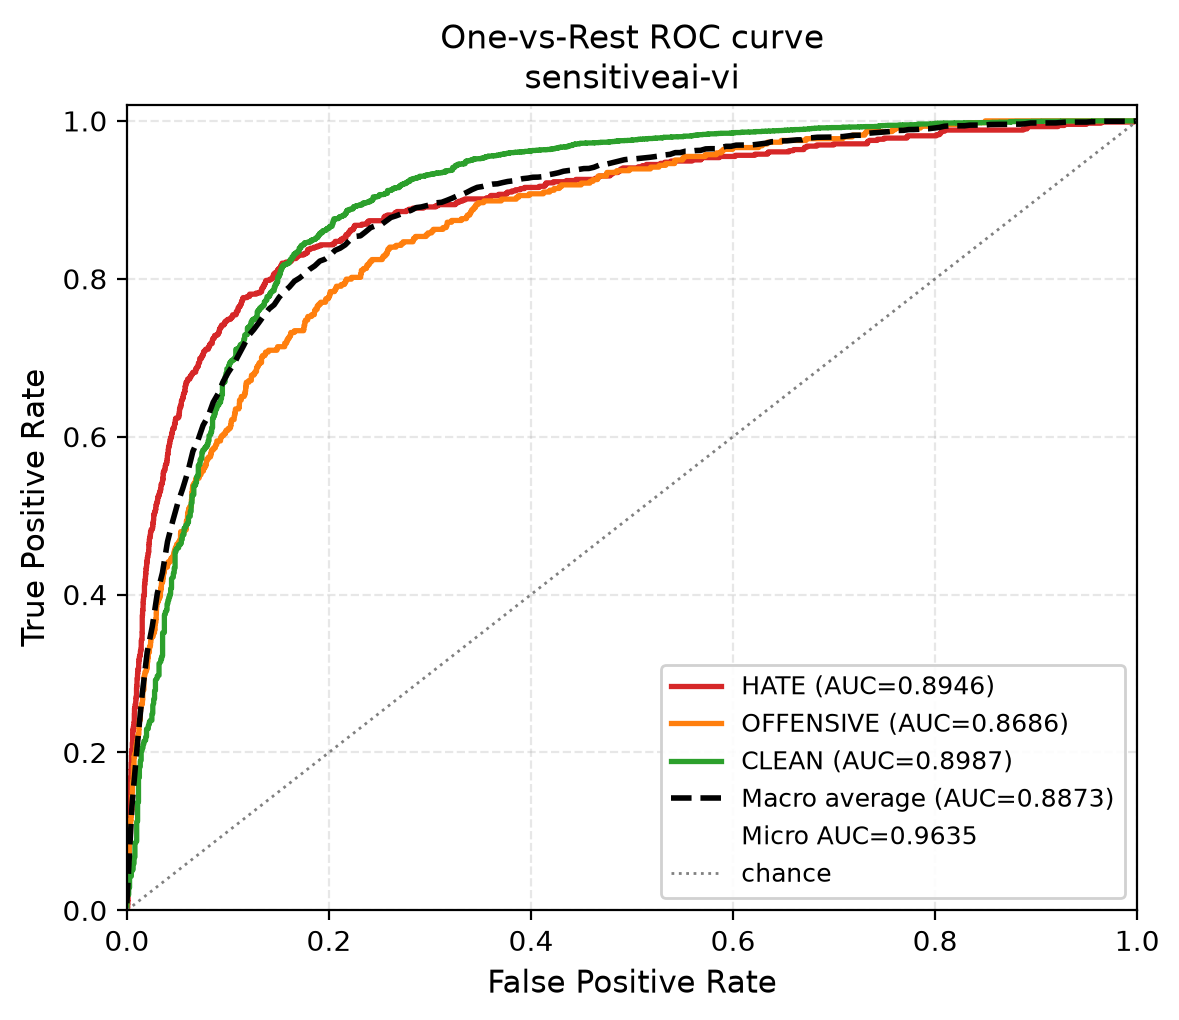
\includegraphics[width=\linewidth]{figures/per_model/M1/roc_curve.png}\caption{ROC curve.}\end{minipage}
\end{figure}

\begin{figure}[htbp]
\centering
\begin{minipage}{0.74\textwidth}\centering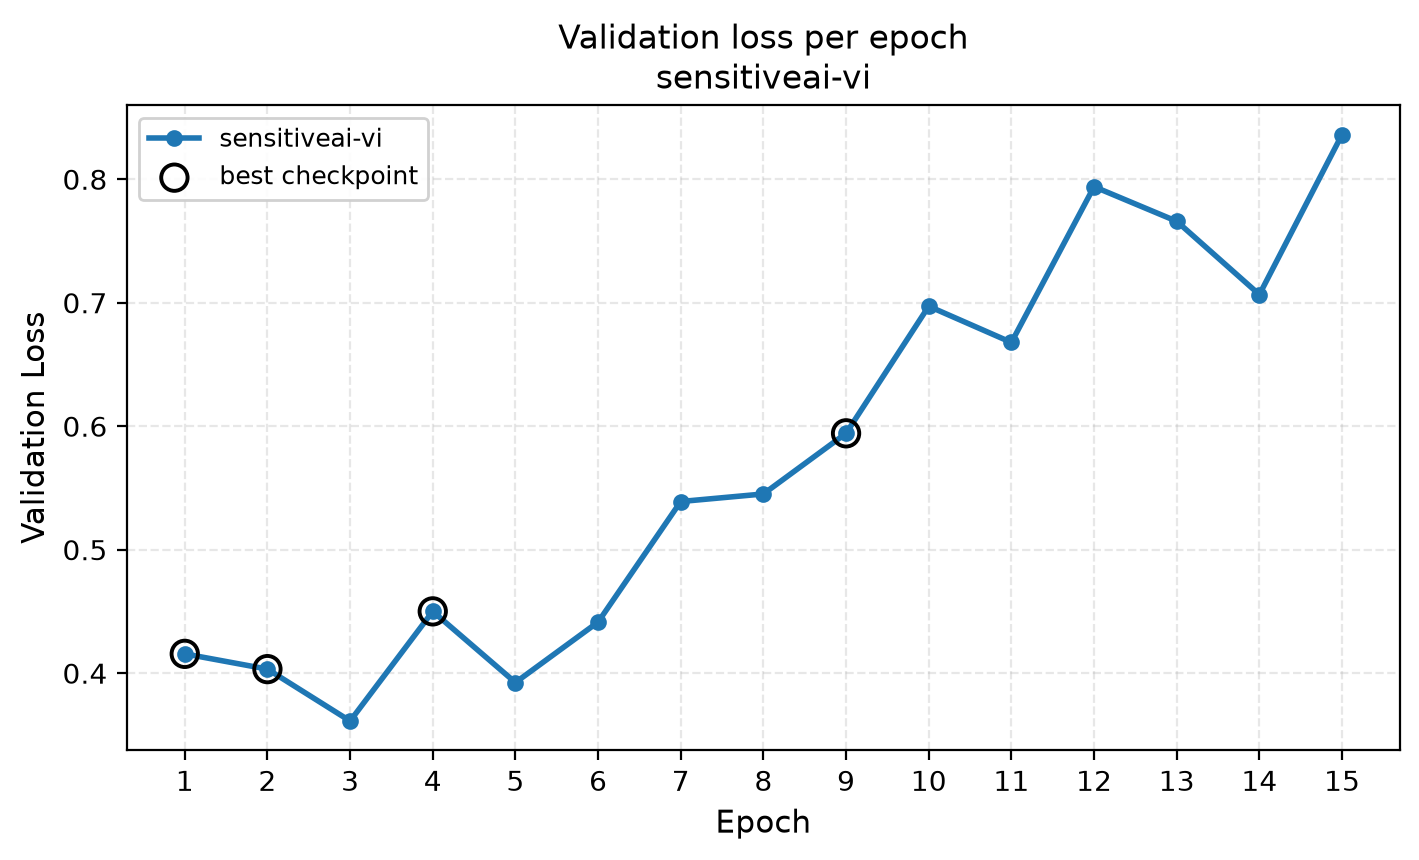
\includegraphics[width=\linewidth]{figures/per_model/M1/val_loss_curve.png}\caption{Validation loss over the training epochs.}\end{minipage}
\end{figure}

\begin{figure}[htbp]
\centering
\begin{minipage}{0.74\textwidth}\centering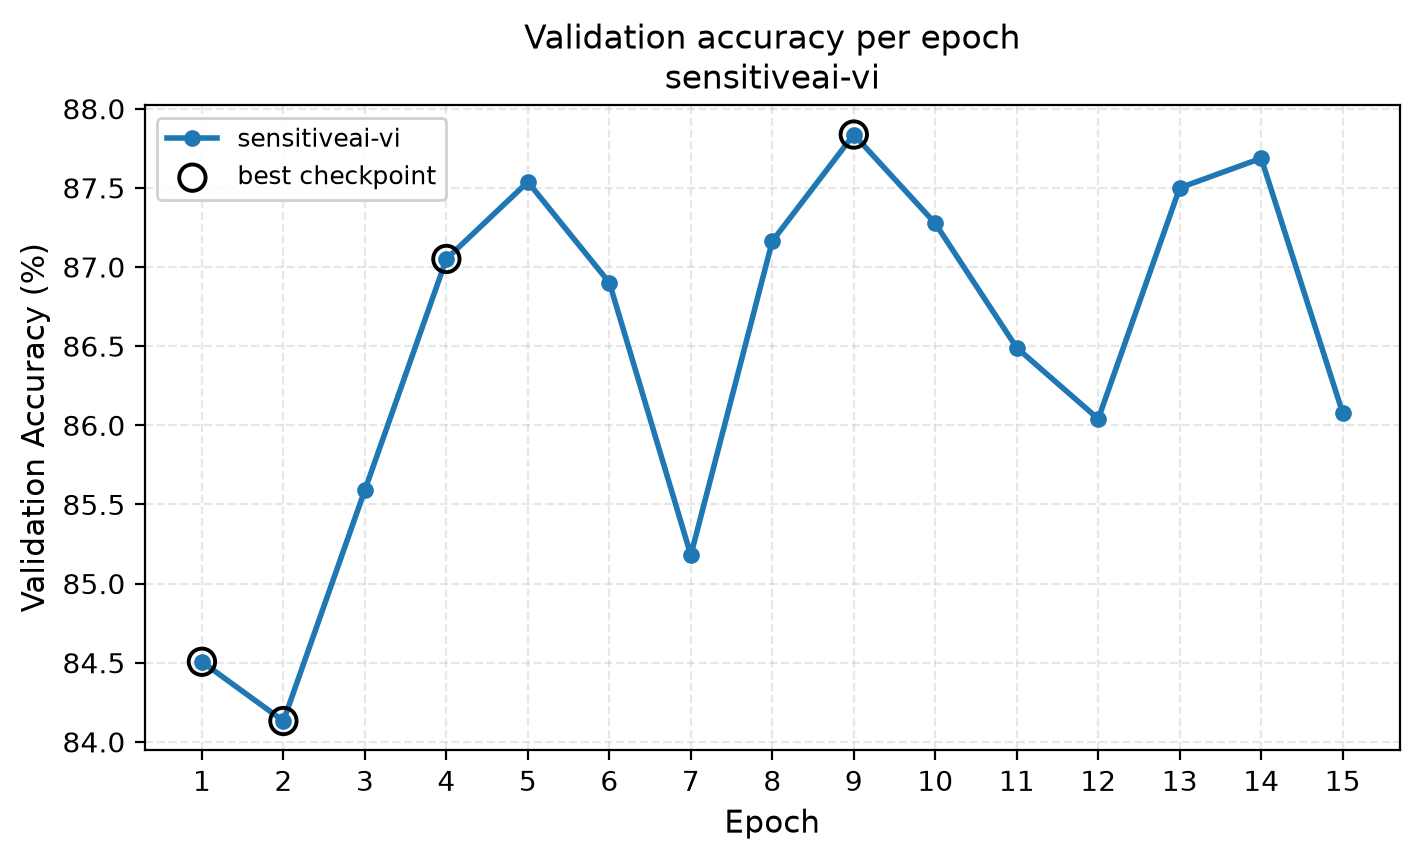
\includegraphics[width=\linewidth]{figures/per_model/M1/val_accuracy_curve.png}\caption{Validation accuracy over the training epochs.}\end{minipage}
\end{figure}


\subsection{\model{M2}}
\label{sec:supp-per-m2}
Baseline plus a \emph{multi-view pooling} head: the first token (\texttt{[CLS]}), masked-mean and masked-max views are concatenated to a 2{,}304-d vector and passed through a LayerNorm $\to$ Linear($2304\to512$) $\to$ GELU $\to$ dropout bottleneck MLP ($512\to3$).  There is no convolutional layer and the optional attention-pooling view is disabled; training is single-stage with plain cross-entropy.

\begin{figure}[htbp]
\centering
\begin{minipage}{0.74\textwidth}\centering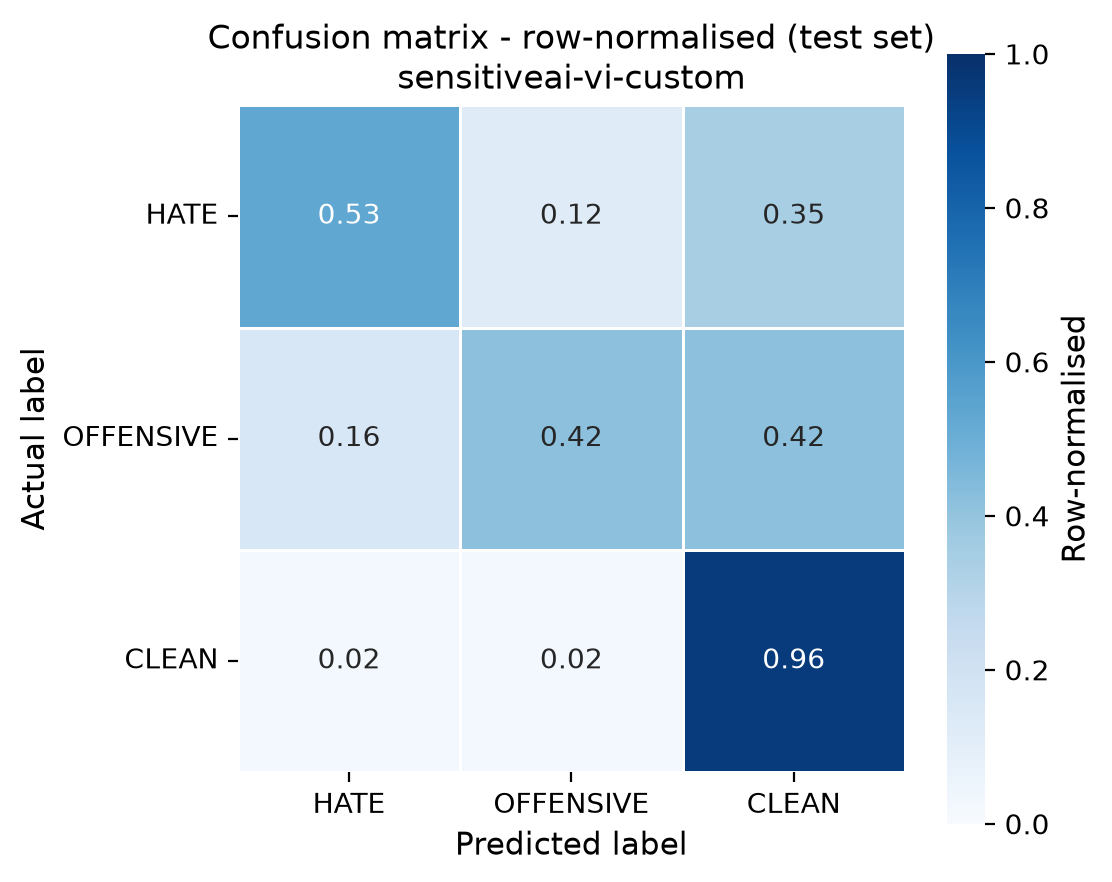
\includegraphics[width=\linewidth]{figures/per_model/M2/confusion_matrix_normalized.png}\caption{Normalised confusion matrix (rows = true, columns = predicted).}\end{minipage}
\end{figure}

\begin{figure}[htbp]
\centering
\begin{minipage}{0.74\textwidth}\centering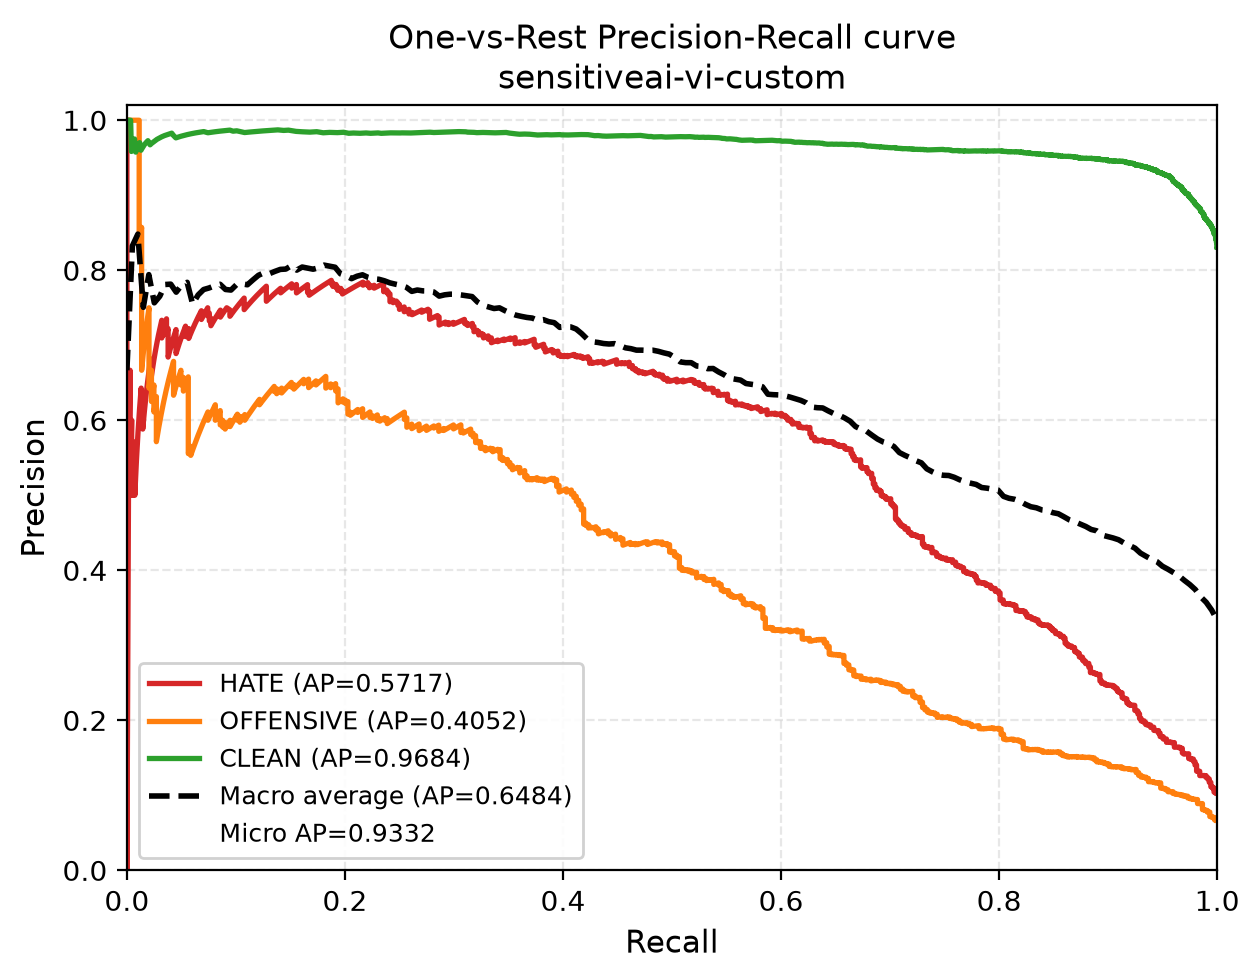
\includegraphics[width=\linewidth]{figures/per_model/M2/pr_curve.png}\caption{Precision--recall curve.}\end{minipage}
\end{figure}

\begin{figure}[htbp]
\centering
\begin{minipage}{0.74\textwidth}\centering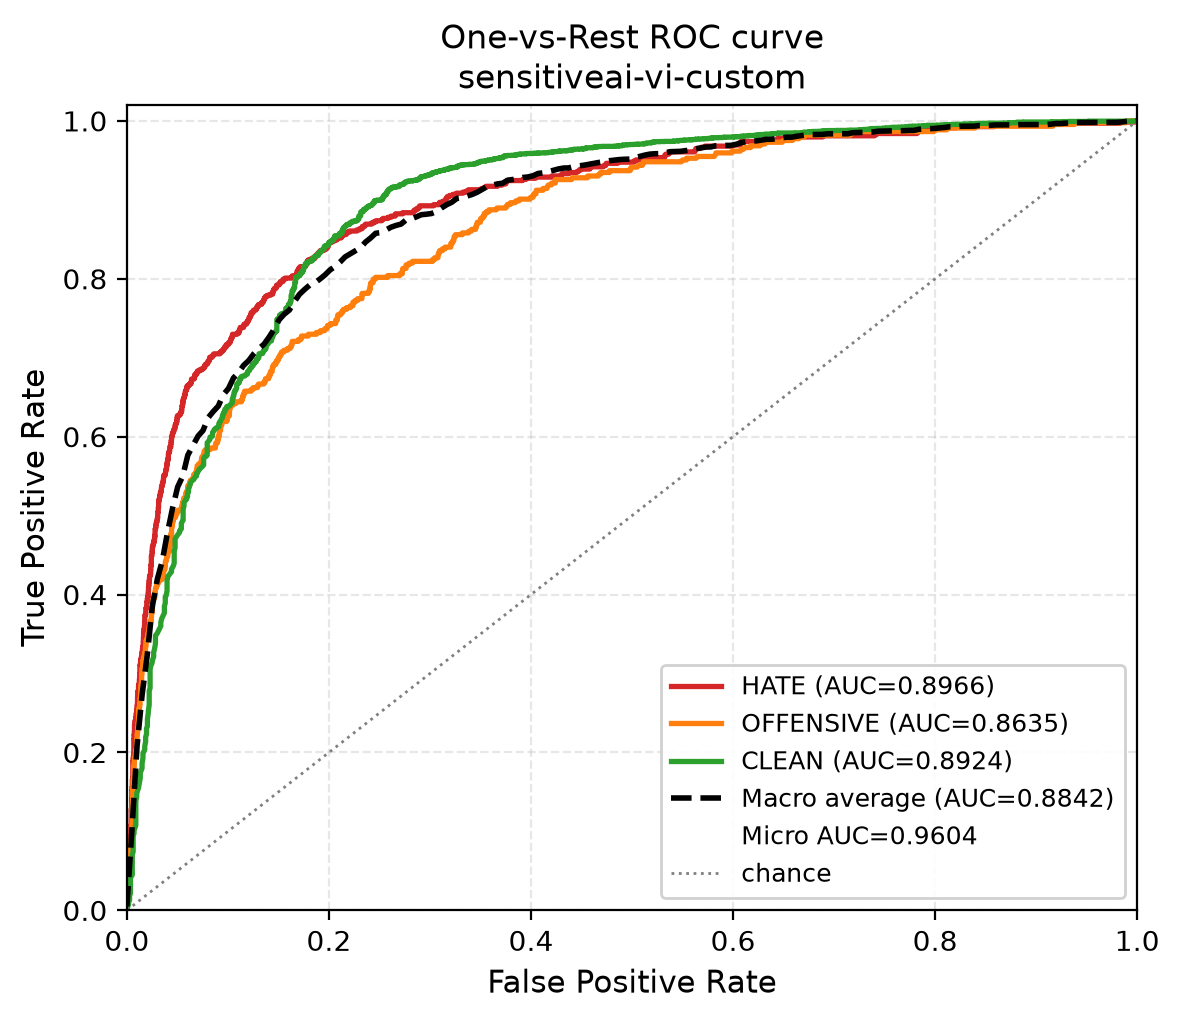
\includegraphics[width=\linewidth]{figures/per_model/M2/roc_curve.png}\caption{ROC curve.}\end{minipage}
\end{figure}

\begin{figure}[htbp]
\centering
\begin{minipage}{0.74\textwidth}\centering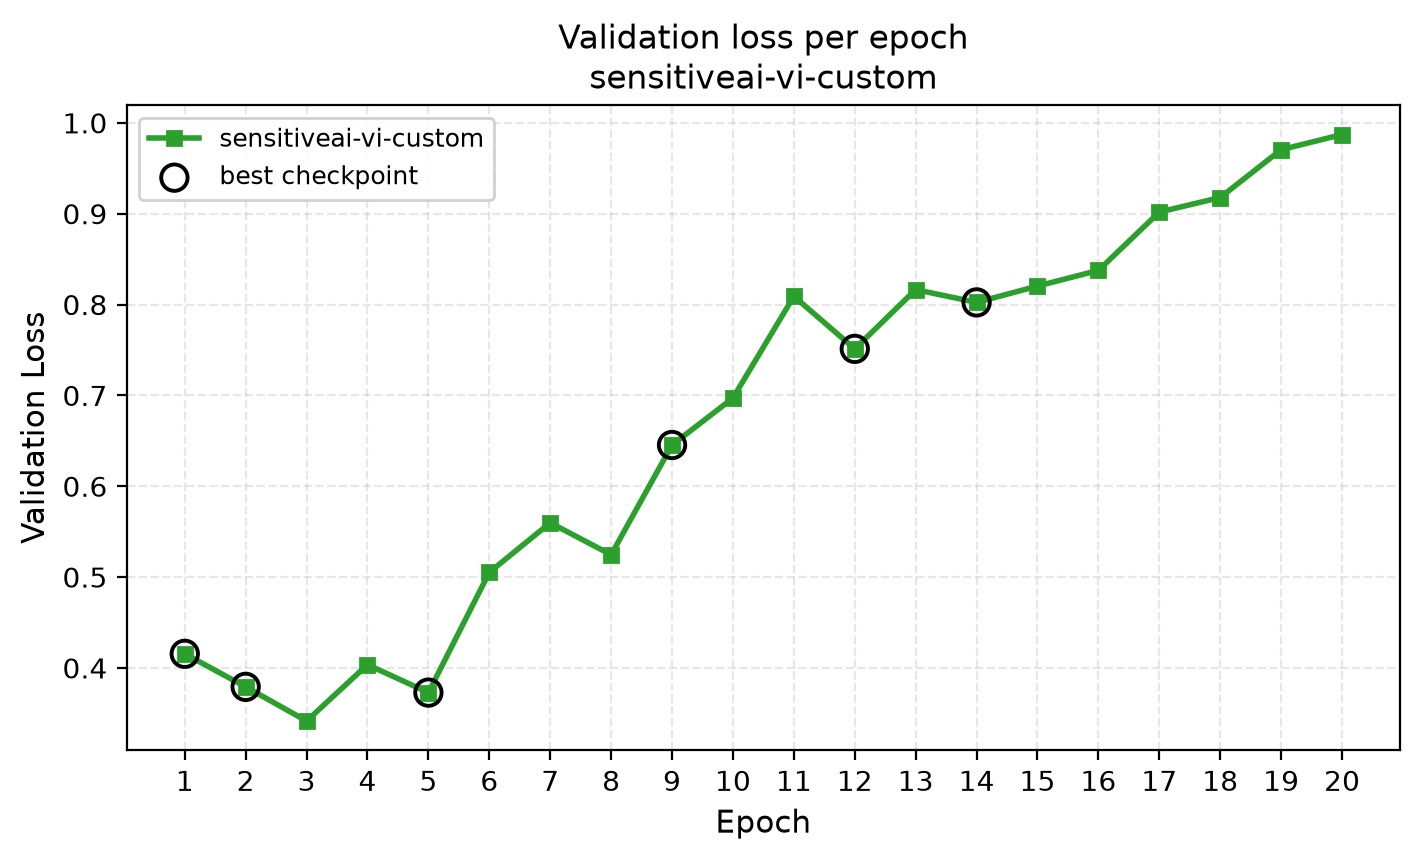
\includegraphics[width=\linewidth]{figures/per_model/M2/val_loss_curve.png}\caption{Validation loss over the training epochs.}\end{minipage}
\end{figure}

\begin{figure}[htbp]
\centering
\begin{minipage}{0.74\textwidth}\centering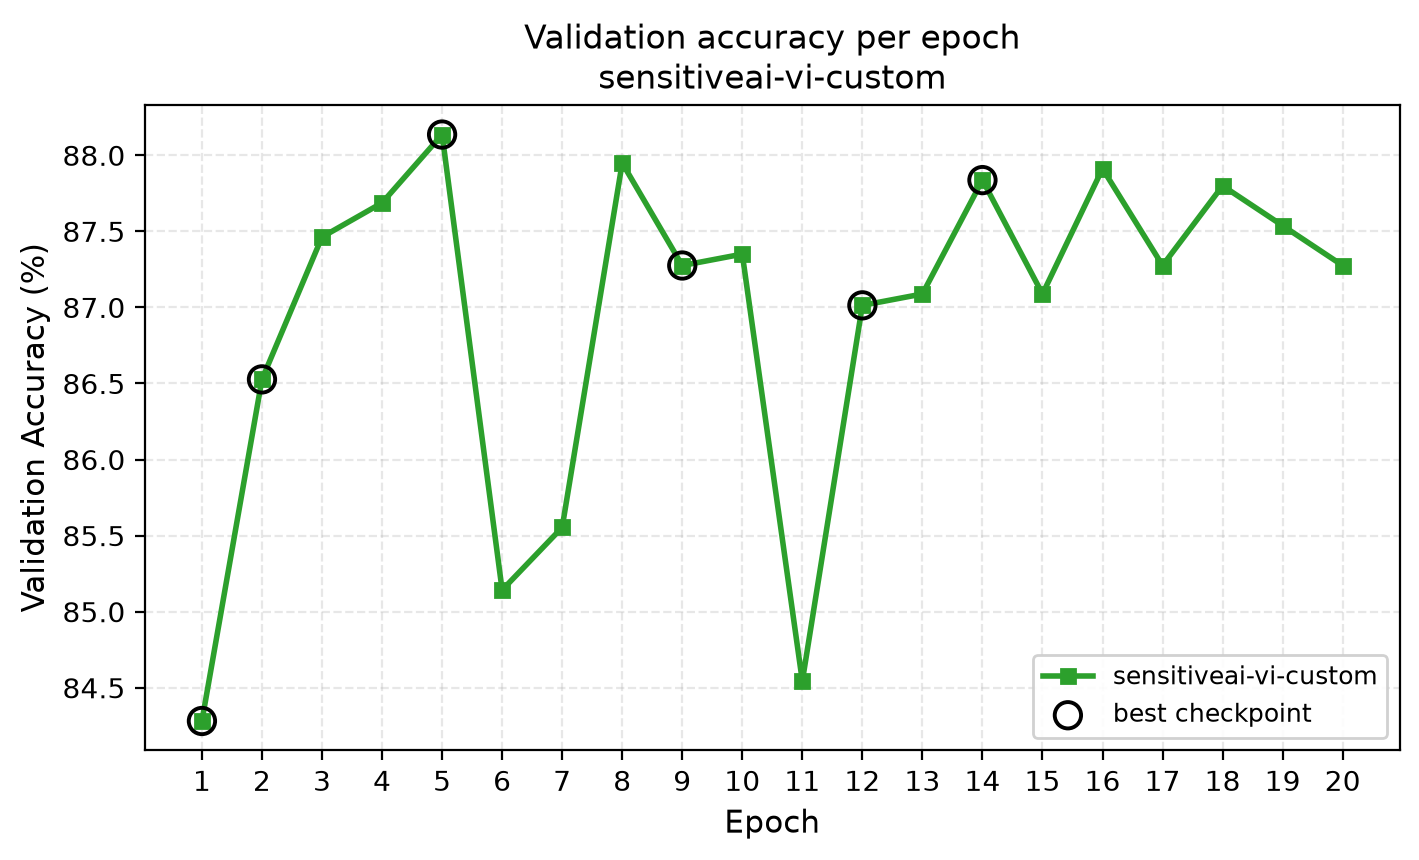
\includegraphics[width=\linewidth]{figures/per_model/M2/val_accuracy_curve.png}\caption{Validation accuracy over the training epochs.}\end{minipage}
\end{figure}


\subsection{\model{M3}}
\label{sec:supp-per-m3}
Multi-view pooling head with discriminative learning rates and a second focal-loss stage; the best macro-F1 of the six ($0.6638$) and the highest MCC.  Its threshold search returned the trivial $0.5$.

\begin{figure}[htbp]
\centering
\begin{minipage}{0.74\textwidth}\centering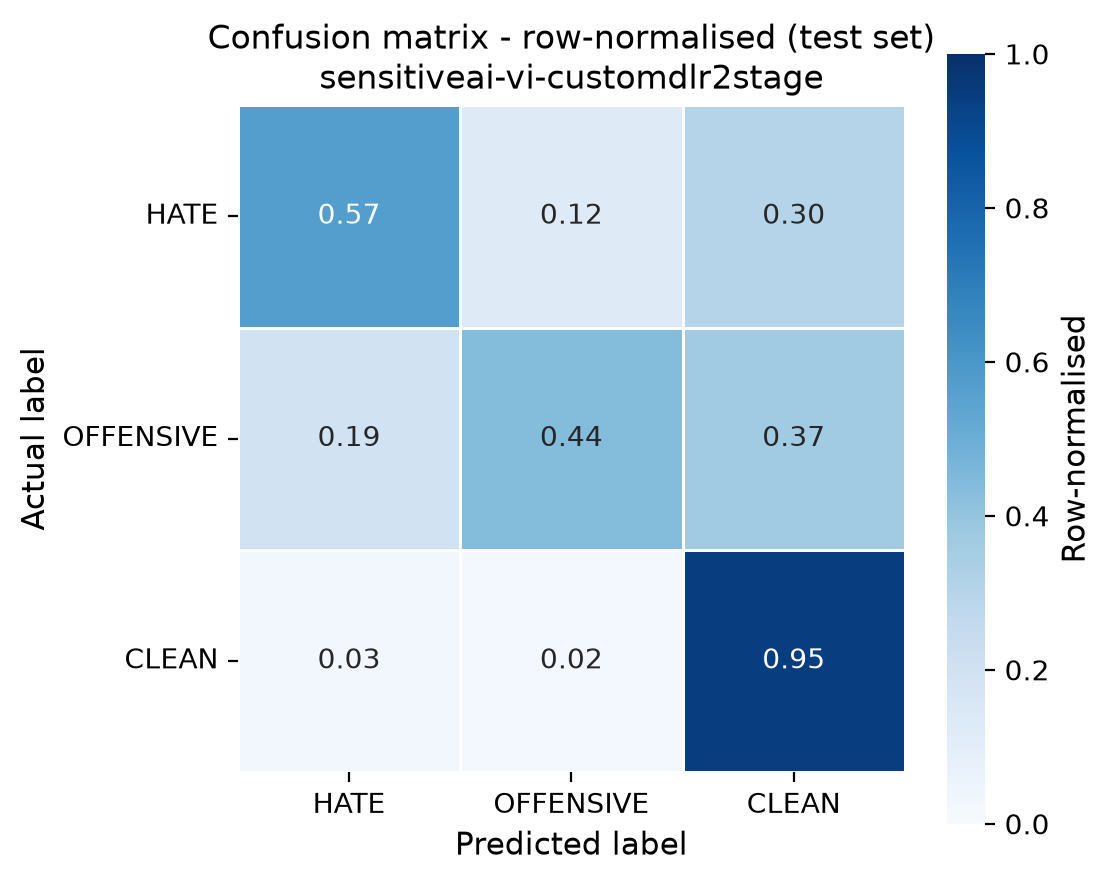
\includegraphics[width=\linewidth]{figures/per_model/M3/confusion_matrix_normalized.png}\caption{Normalised confusion matrix (rows = true, columns = predicted).}\end{minipage}
\end{figure}

\begin{figure}[htbp]
\centering
\begin{minipage}{0.74\textwidth}\centering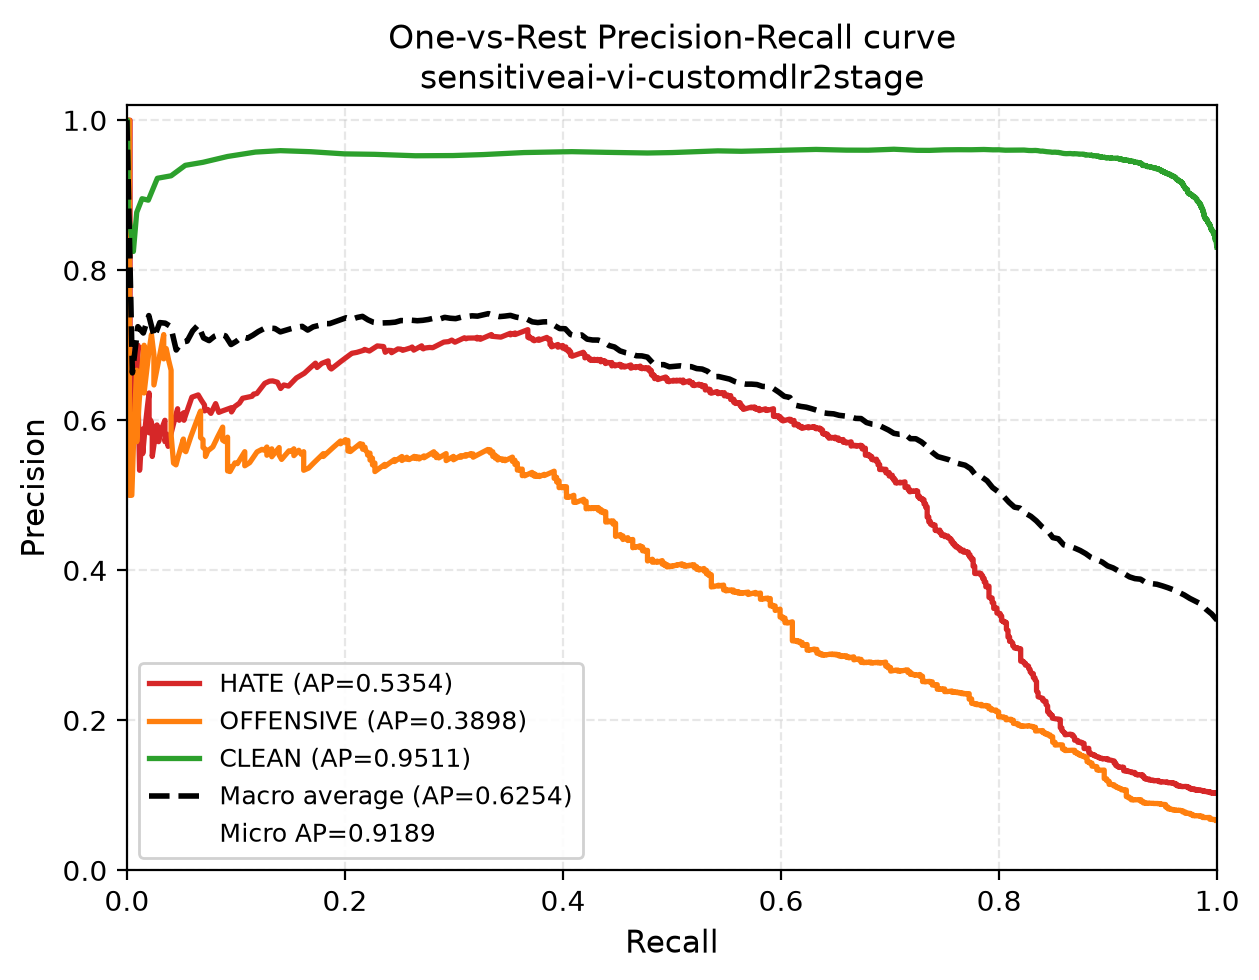
\includegraphics[width=\linewidth]{figures/per_model/M3/pr_curve.png}\caption{Precision--recall curve.}\end{minipage}
\end{figure}

\begin{figure}[htbp]
\centering
\begin{minipage}{0.74\textwidth}\centering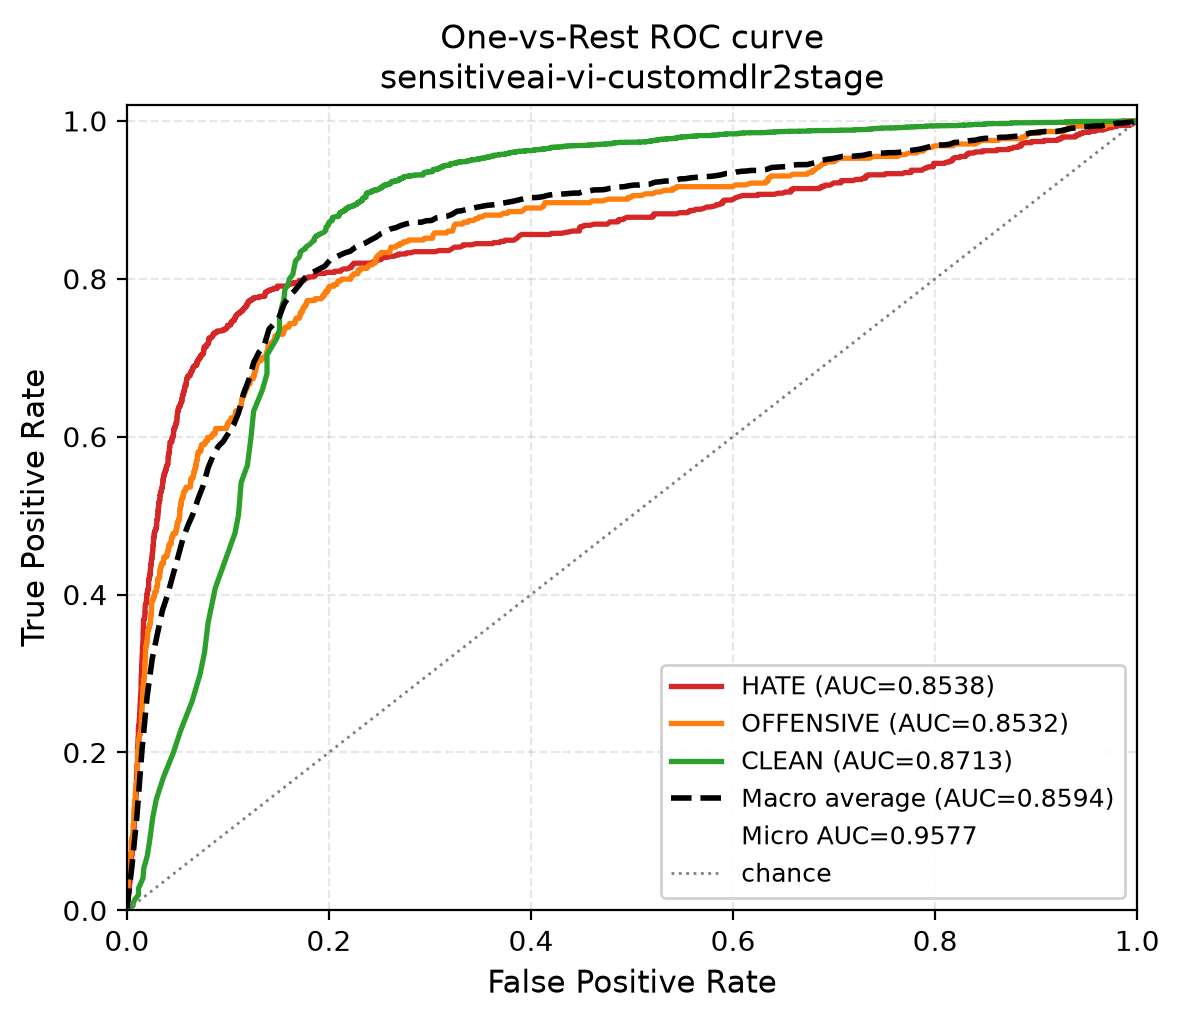
\includegraphics[width=\linewidth]{figures/per_model/M3/roc_curve.png}\caption{ROC curve.}\end{minipage}
\end{figure}

\begin{figure}[htbp]
\centering
\begin{minipage}{0.74\textwidth}\centering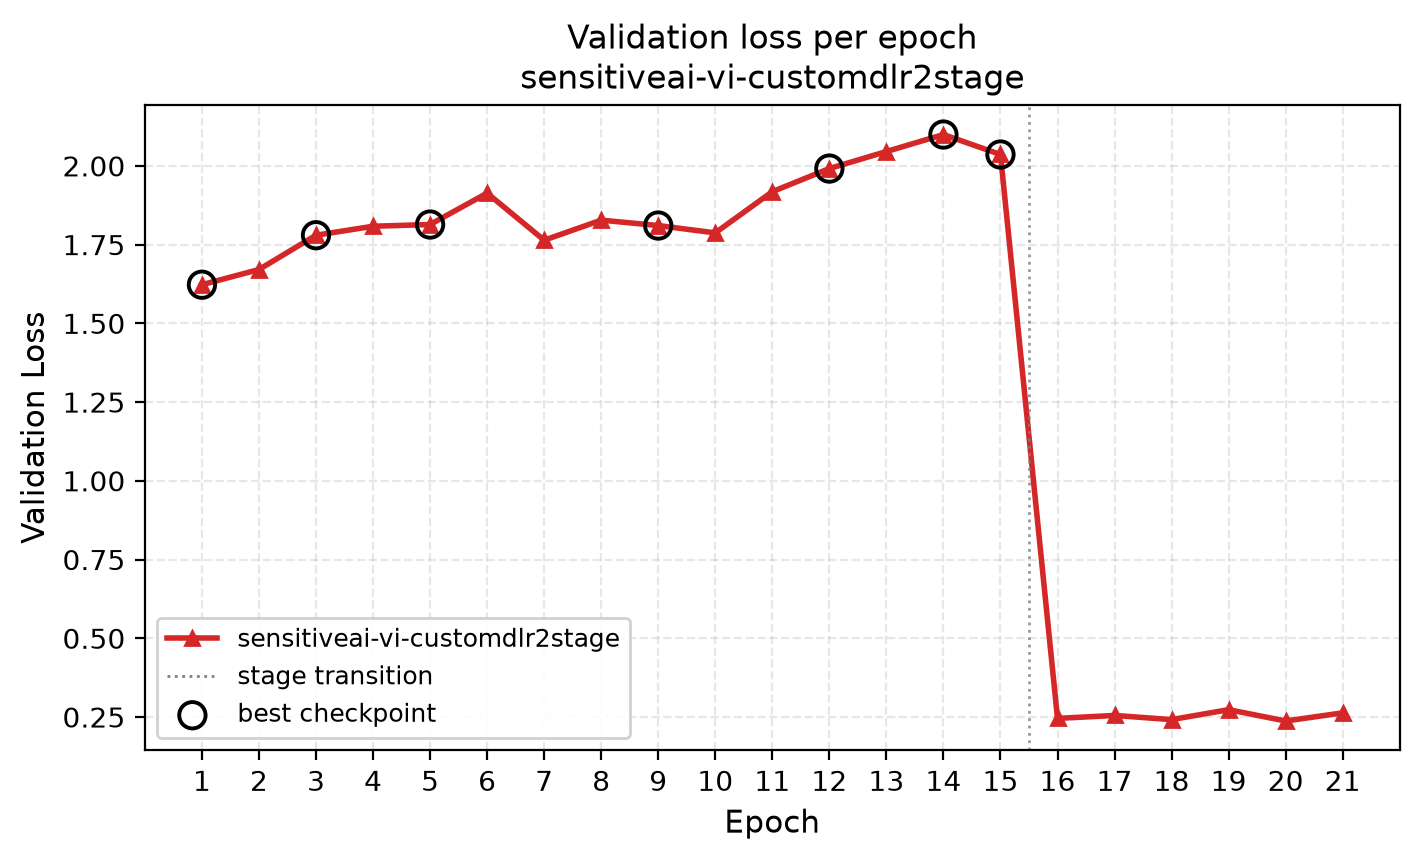
\includegraphics[width=\linewidth]{figures/per_model/M3/val_loss_curve.png}\caption{Validation loss over the training epochs.}\end{minipage}
\end{figure}

\begin{figure}[htbp]
\centering
\begin{minipage}{0.74\textwidth}\centering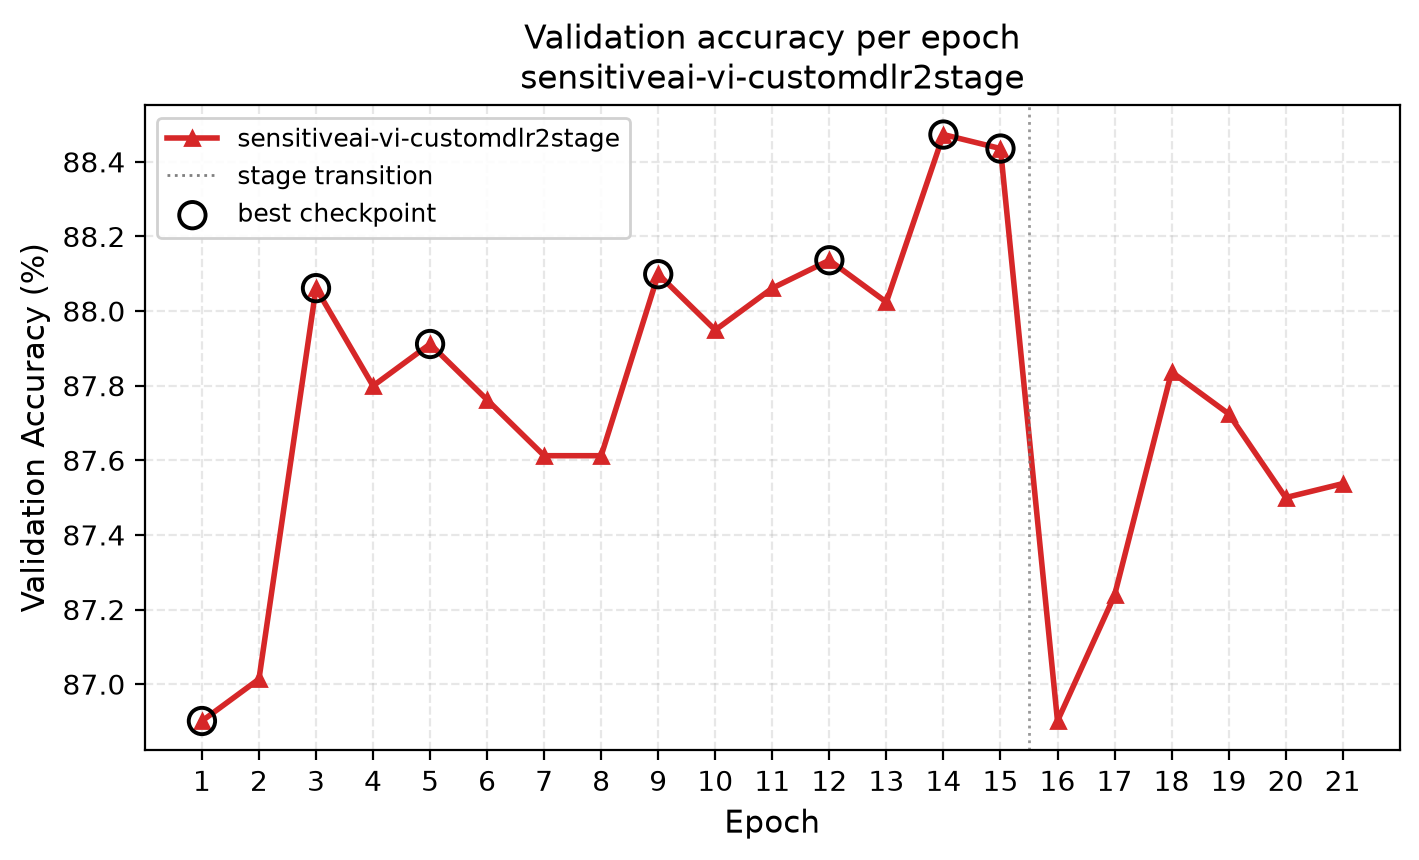
\includegraphics[width=\linewidth]{figures/per_model/M3/val_accuracy_curve.png}\caption{Validation accuracy over the training epochs.}\end{minipage}
\end{figure}


\subsection{\model{M4}}
\label{sec:supp-per-m4}
Multi-view head trained as a three-stage curriculum, initialised from \model{M3}'s checkpoint.  Stage~1 (concept loss, OFFENSIVE) was allocated 10 epochs but early stopping truncated it after 7; stage~2 (concept loss, HATE) ran 6\,(absolute epochs $8$--$13$) and stage~3 (cross-entropy, class weights $3{:}2{:}1$) ran 6\,(absolute epochs $14$--$19$), for $19$ of $30$ planned epochs.  The run's best \emph{validation} macro-F1 ($0.6942$) occurred at absolute epoch~1 and was never beaten, so the later stages were not selected; its searched thresholds ($0.01/0.5/0.64$) raised validation macro-F1 but did not transfer to test.

\begin{figure}[htbp]
\centering
\begin{minipage}{0.74\textwidth}\centering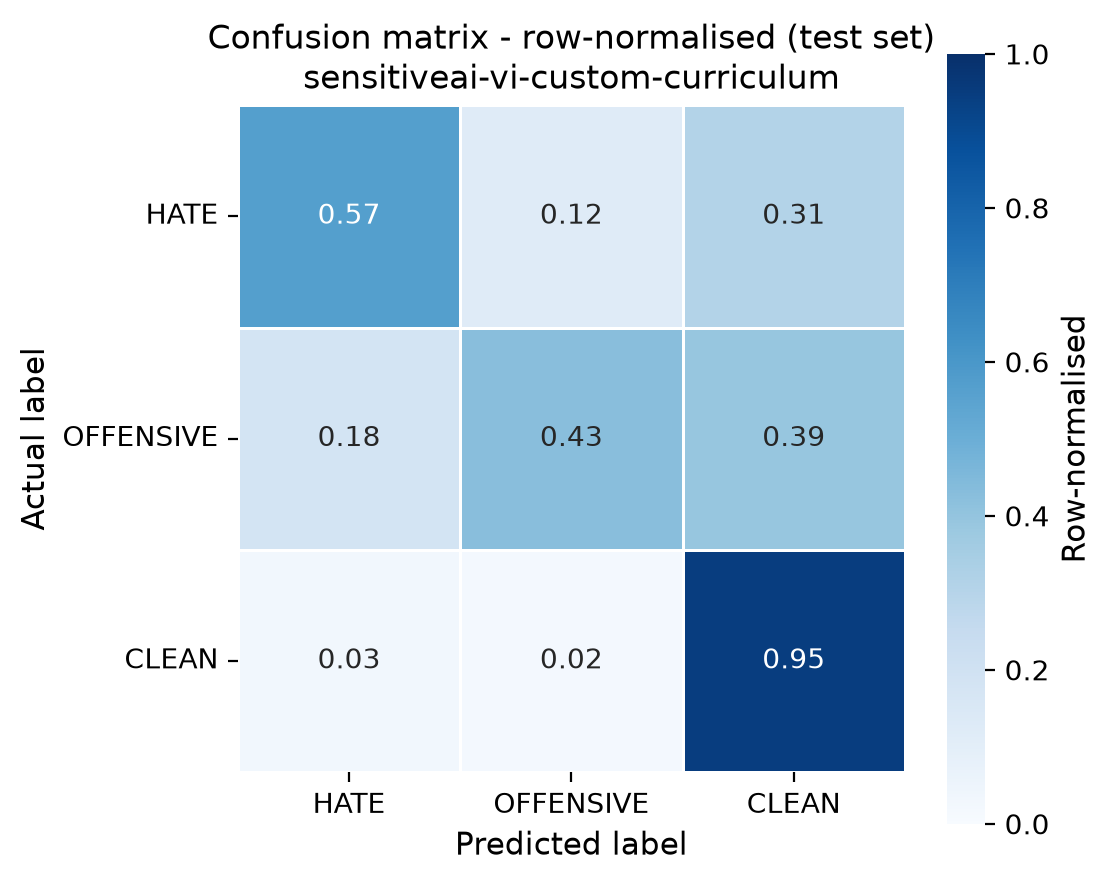
\includegraphics[width=\linewidth]{figures/per_model/M4/confusion_matrix_normalized.png}\caption{Normalised confusion matrix (rows = true, columns = predicted).}\end{minipage}
\end{figure}

\begin{figure}[htbp]
\centering
\begin{minipage}{0.74\textwidth}\centering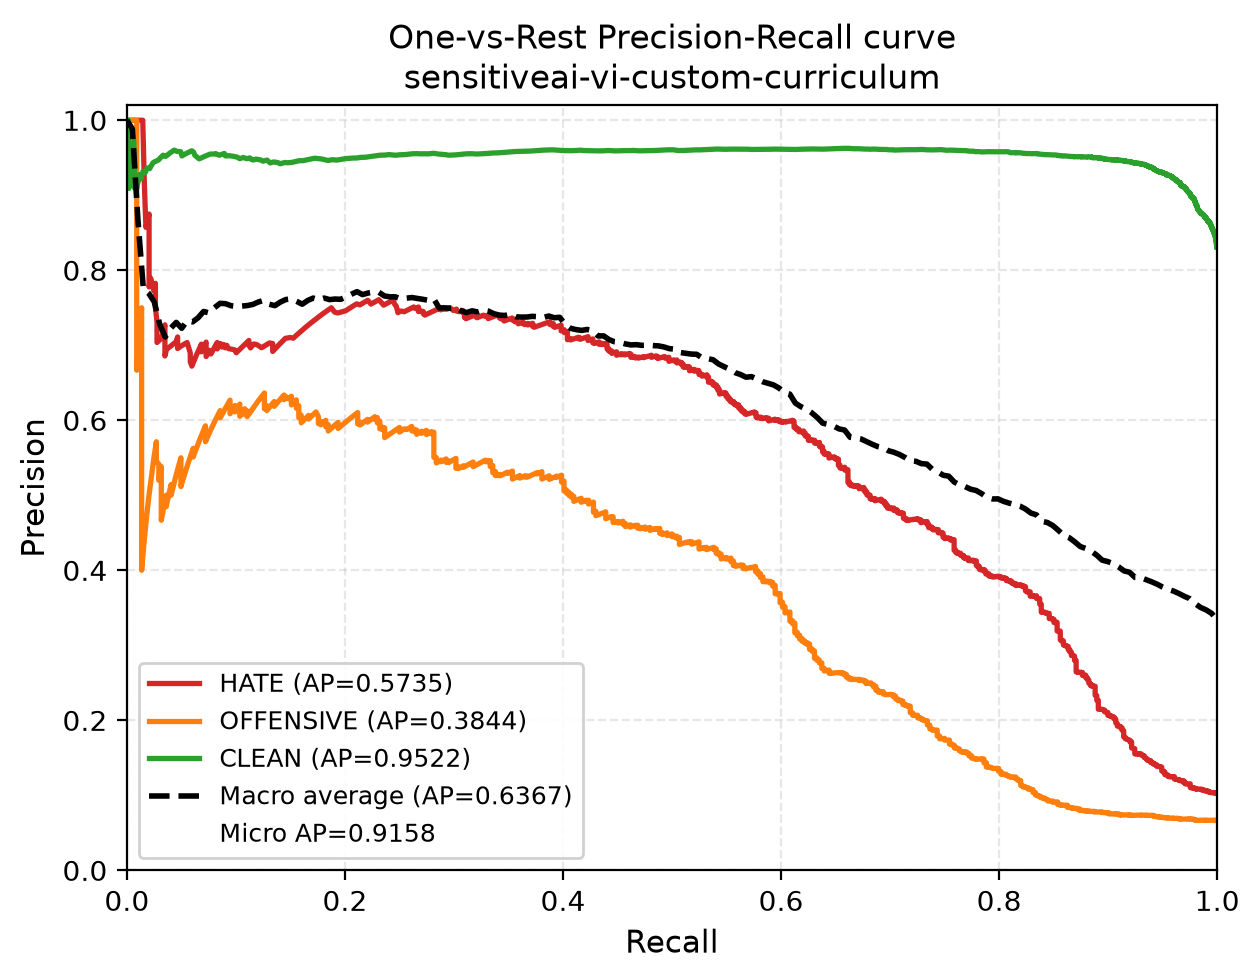
\includegraphics[width=\linewidth]{figures/per_model/M4/pr_curve.png}\caption{Precision--recall curve.}\end{minipage}
\end{figure}

\begin{figure}[htbp]
\centering
\begin{minipage}{0.74\textwidth}\centering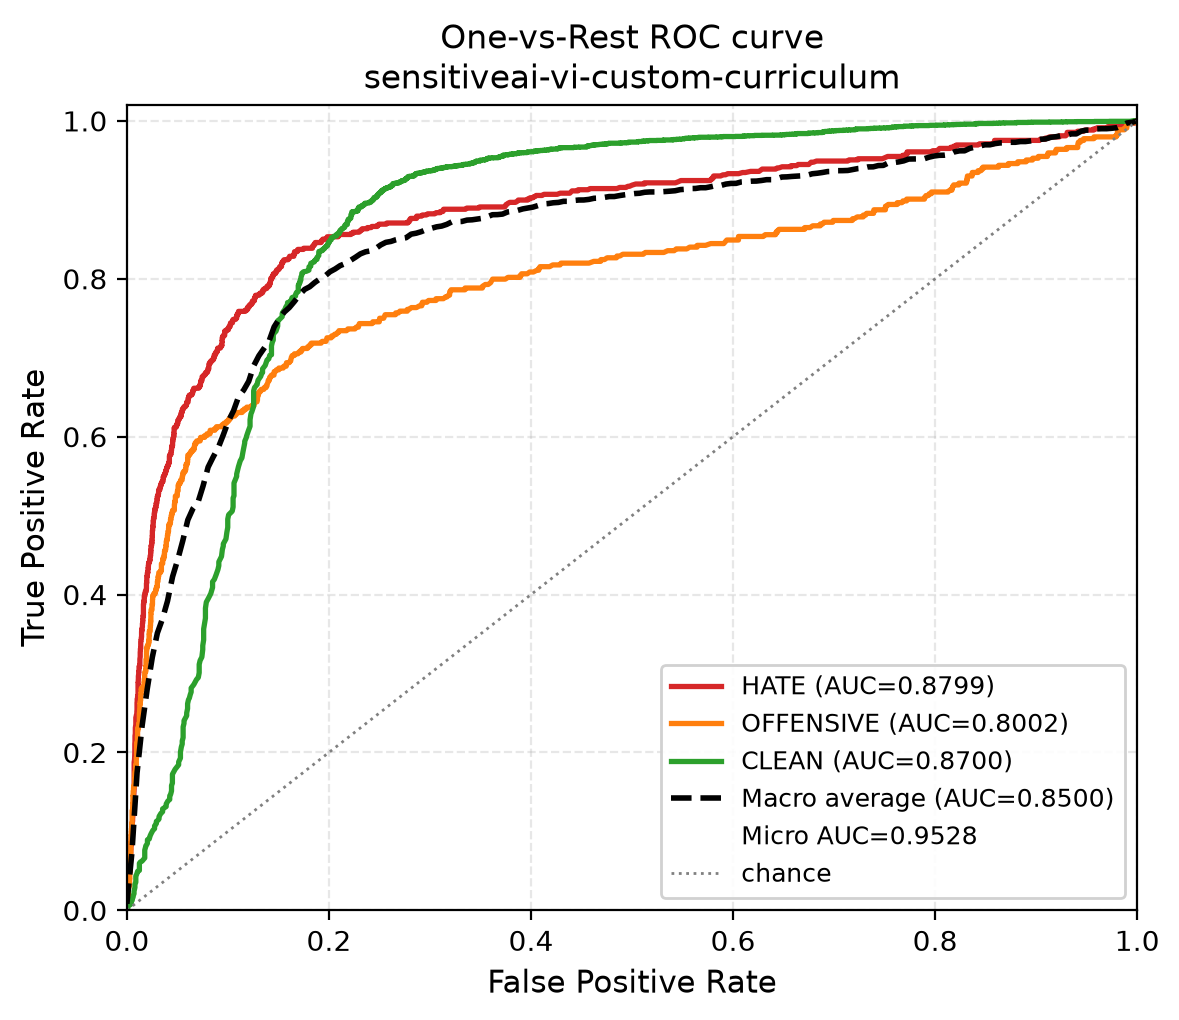
\includegraphics[width=\linewidth]{figures/per_model/M4/roc_curve.png}\caption{ROC curve.}\end{minipage}
\end{figure}

\begin{figure}[htbp]
\centering
\begin{minipage}{0.74\textwidth}\centering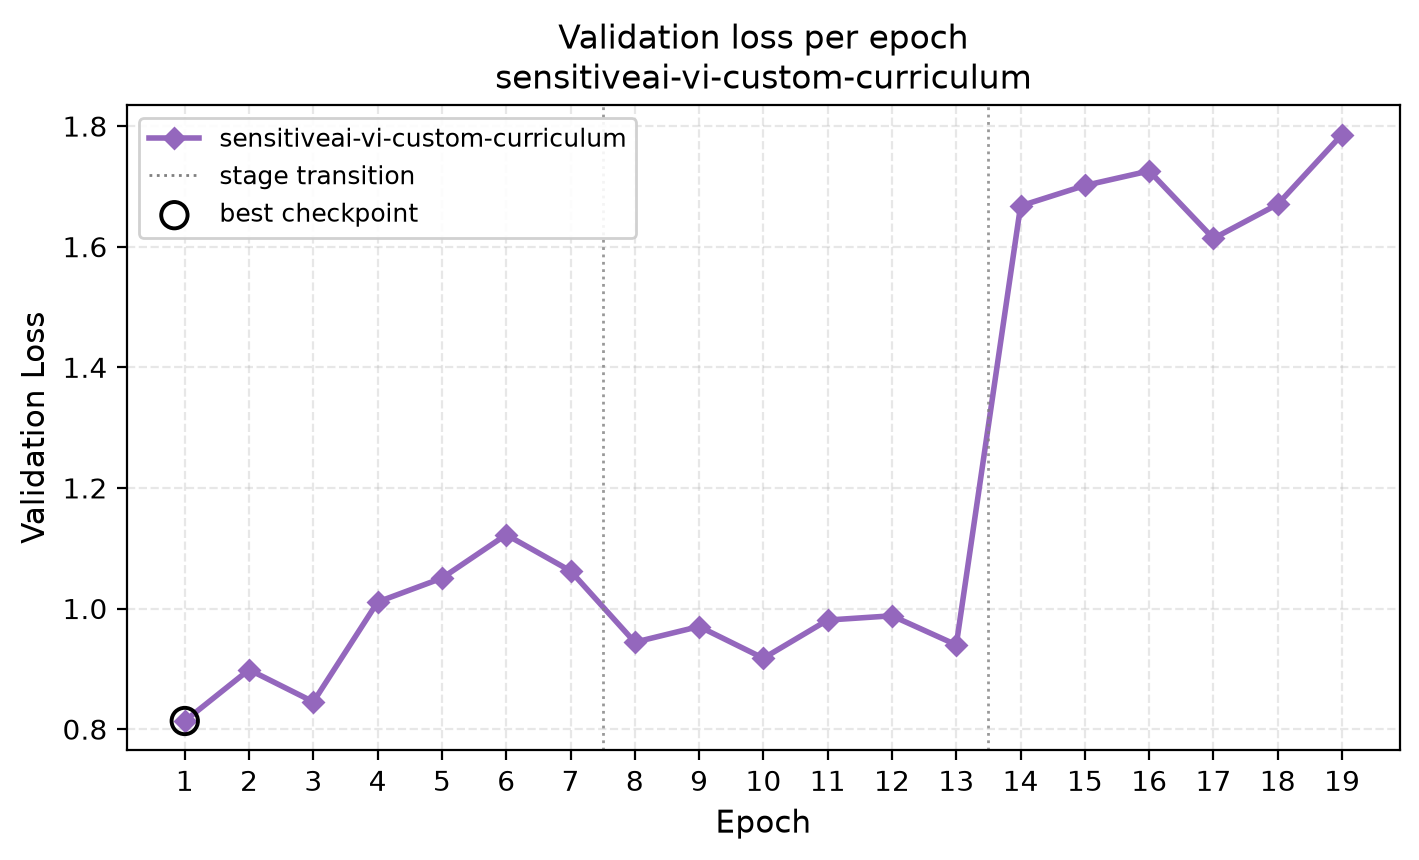
\includegraphics[width=\linewidth]{figures/per_model/M4/val_loss_curve.png}\caption{Validation loss over the training epochs.}\end{minipage}
\end{figure}

\begin{figure}[htbp]
\centering
\begin{minipage}{0.74\textwidth}\centering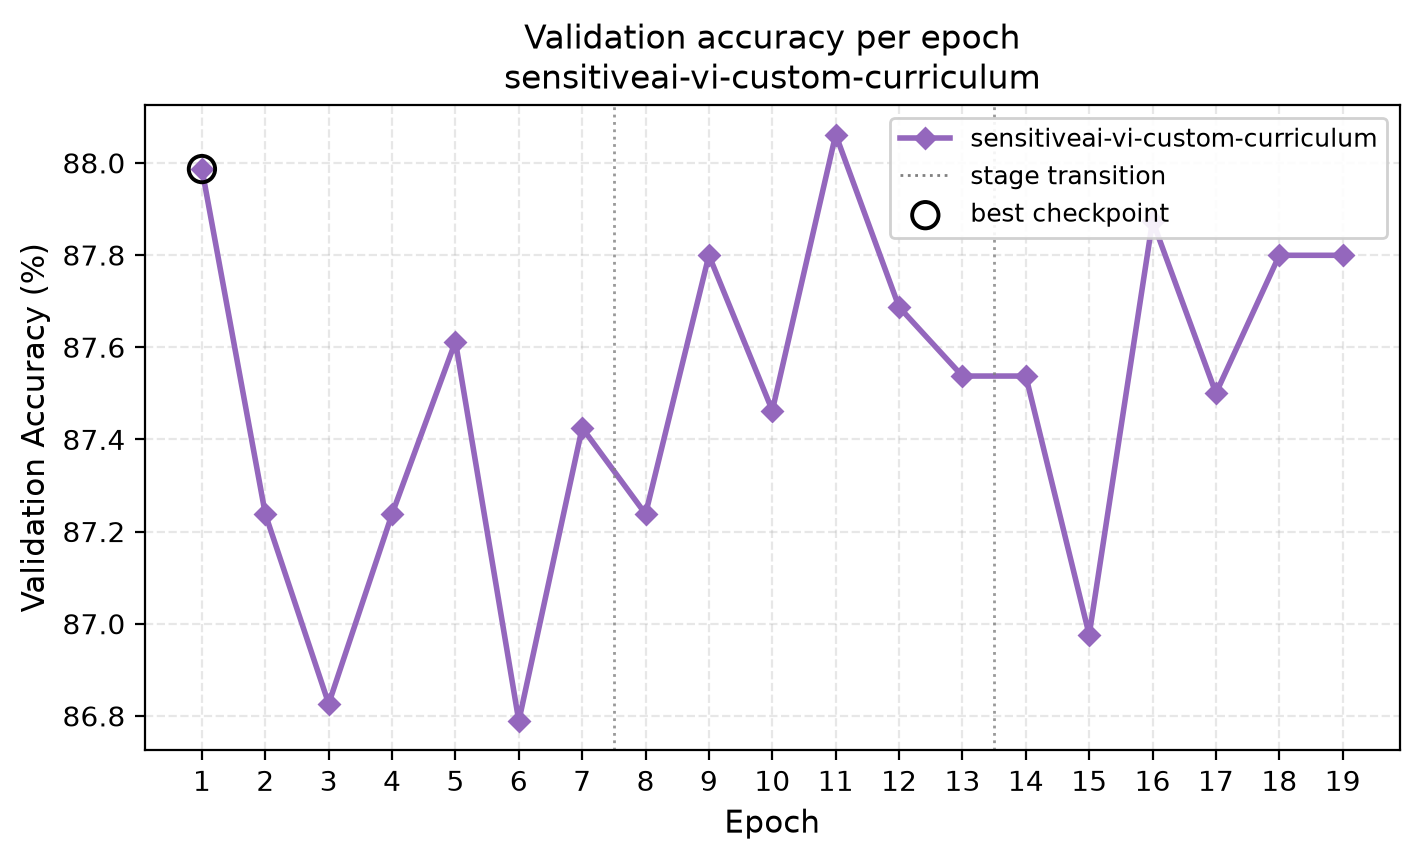
\includegraphics[width=\linewidth]{figures/per_model/M4/val_accuracy_curve.png}\caption{Validation accuracy over the training epochs.}\end{minipage}
\end{figure}


\subsection{\model{M5}}
\label{sec:supp-per-m5}
Continuation of \model{M3}'s stage-1 recipe (DLR plus class-weighted cross-entropy) for a further 15 epochs, reaching the full budget because the early-stopping patience equals the budget and could not trigger earlier.  It has the \emph{highest} test accuracy ($0.878$) but the \emph{lowest} macro-F1 ($0.654$)---the accuracy/macro-F1 trap in one system.

\begin{figure}[htbp]
\centering
\begin{minipage}{0.74\textwidth}\centering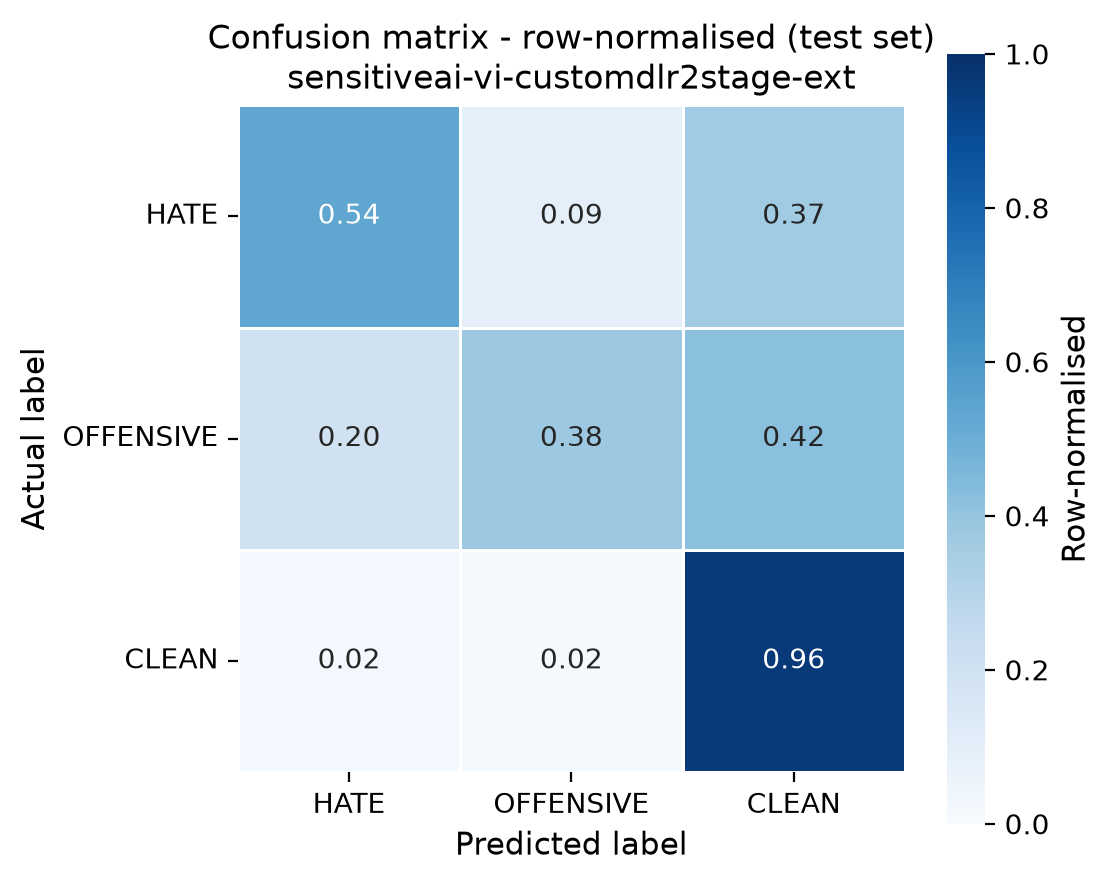
\includegraphics[width=\linewidth]{figures/per_model/M5/confusion_matrix_normalized.png}\caption{Normalised confusion matrix (rows = true, columns = predicted).}\end{minipage}
\end{figure}

\begin{figure}[htbp]
\centering
\begin{minipage}{0.74\textwidth}\centering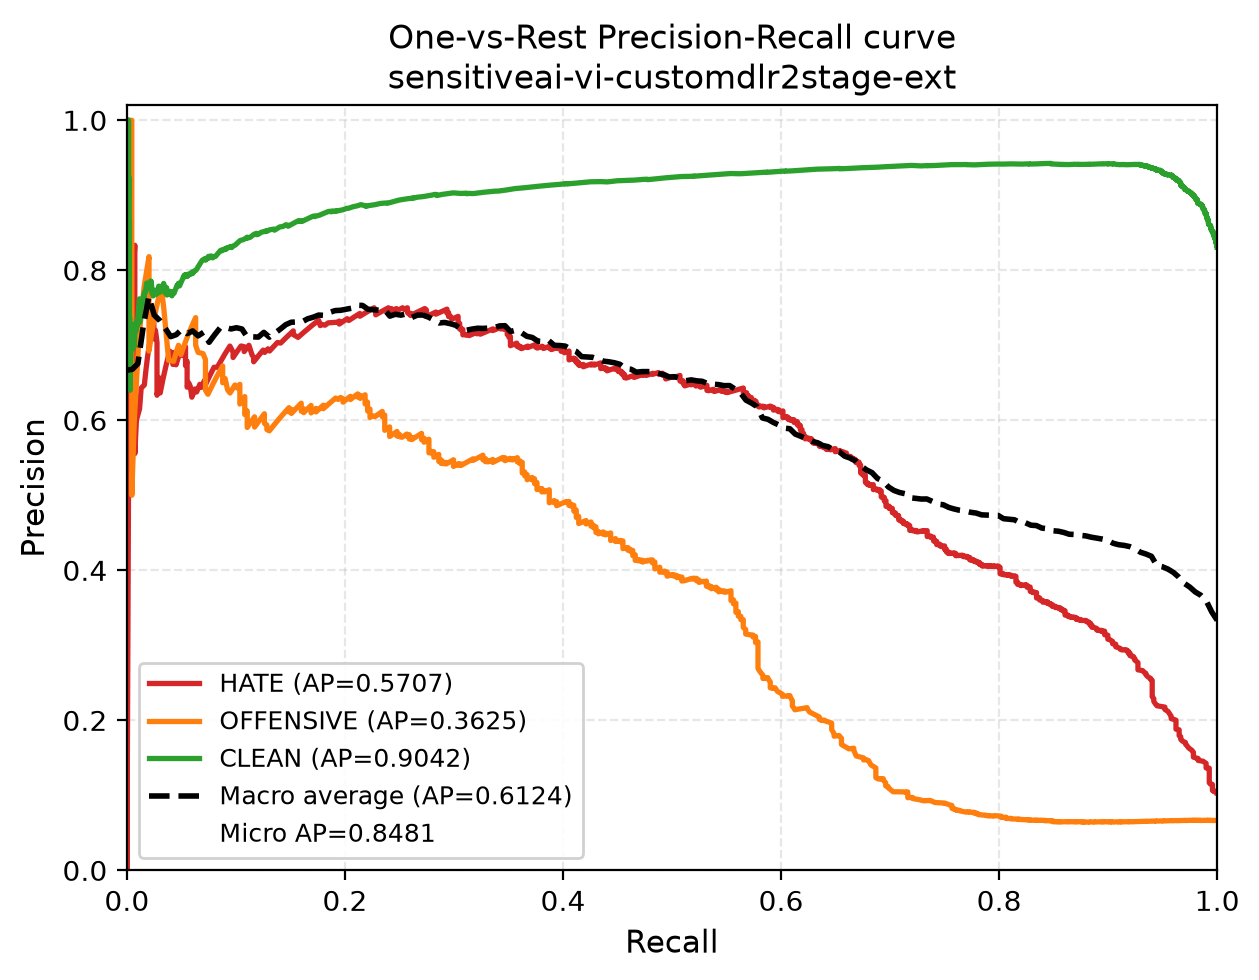
\includegraphics[width=\linewidth]{figures/per_model/M5/pr_curve.png}\caption{Precision--recall curve.}\end{minipage}
\end{figure}

\begin{figure}[htbp]
\centering
\begin{minipage}{0.74\textwidth}\centering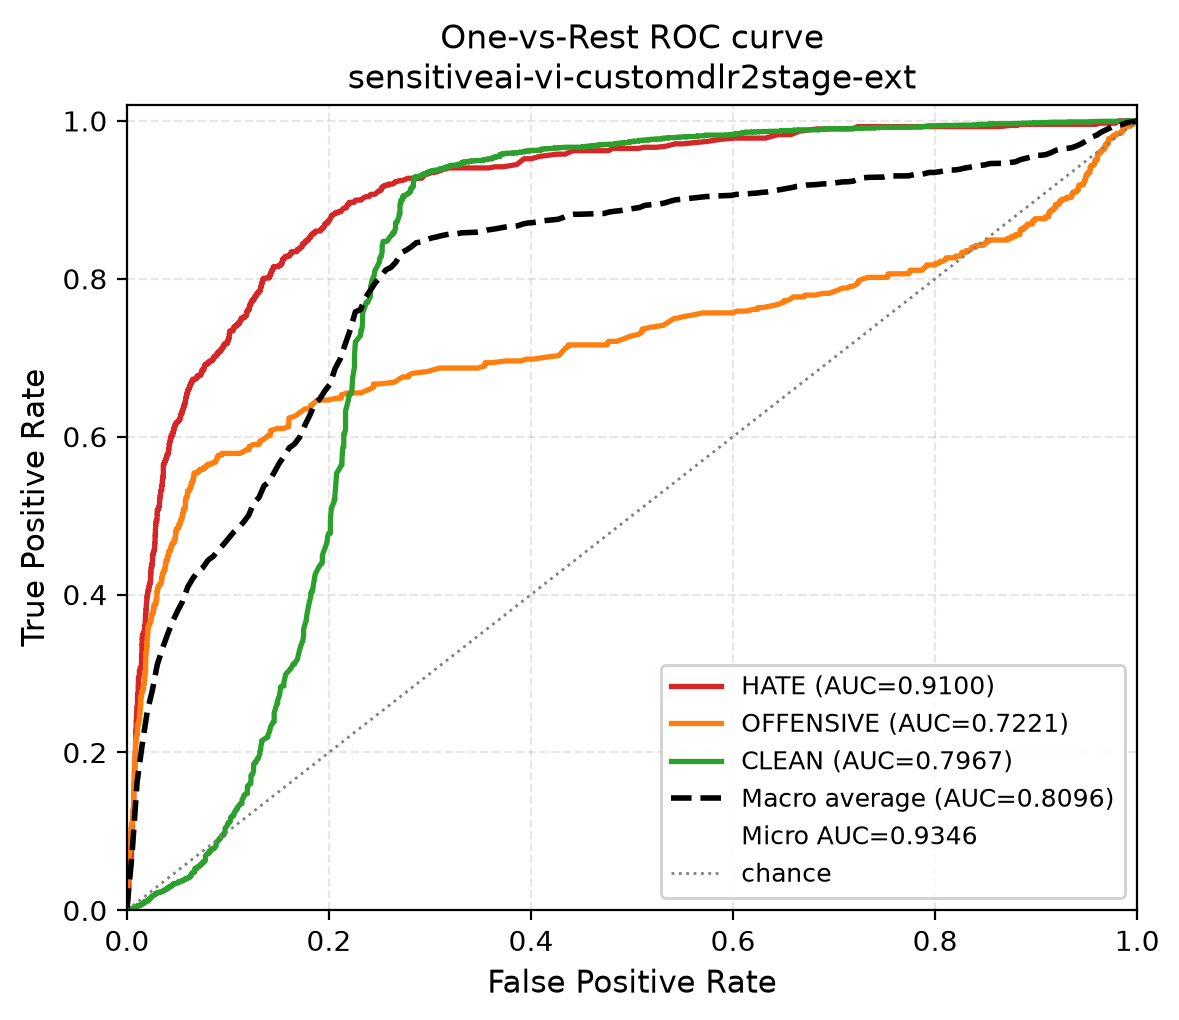
\includegraphics[width=\linewidth]{figures/per_model/M5/roc_curve.png}\caption{ROC curve.}\end{minipage}
\end{figure}

\begin{figure}[htbp]
\centering
\begin{minipage}{0.74\textwidth}\centering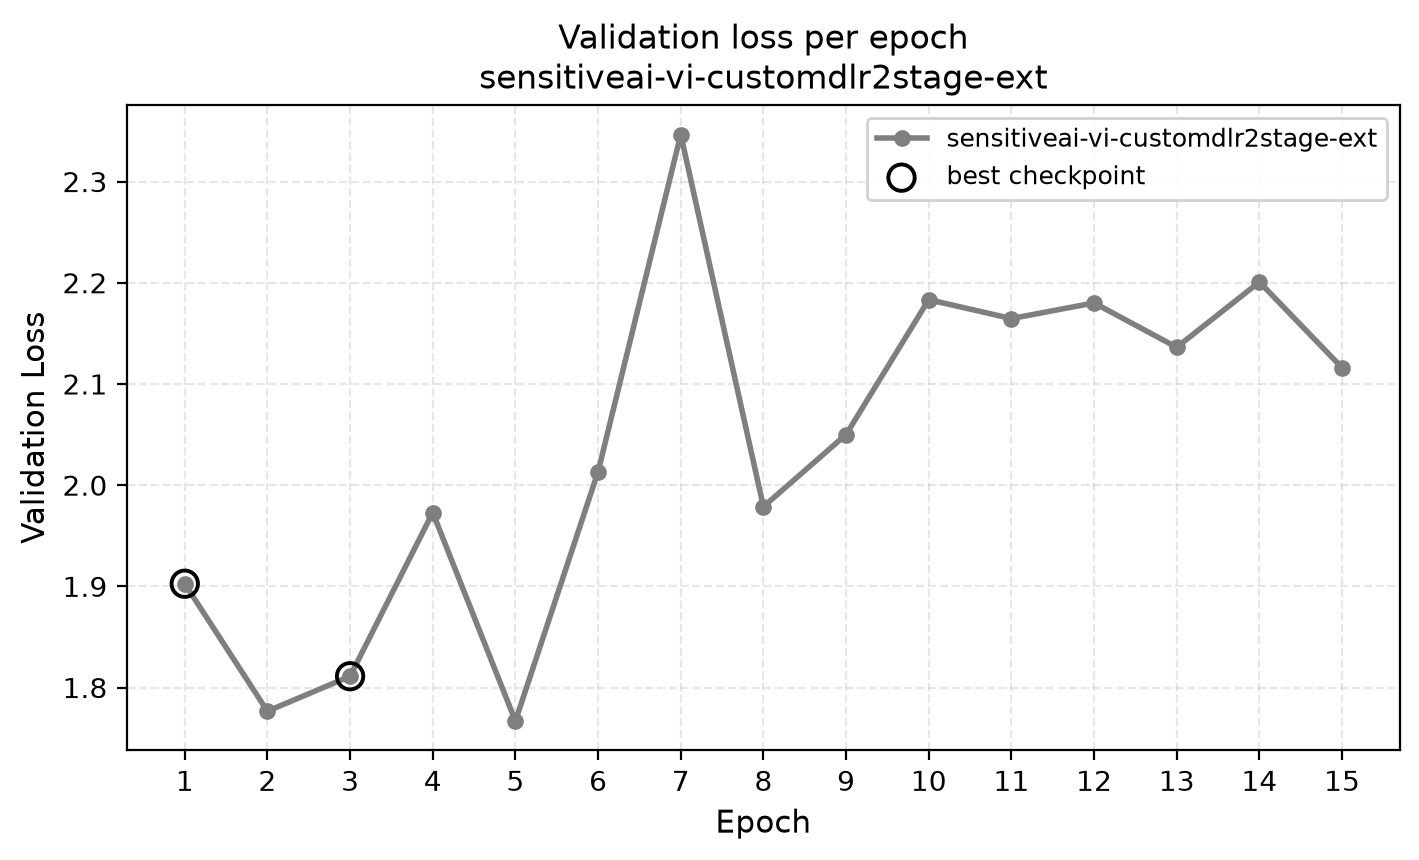
\includegraphics[width=\linewidth]{figures/per_model/M5/val_loss_curve.png}\caption{Validation loss over the training epochs.}\end{minipage}
\end{figure}

\begin{figure}[htbp]
\centering
\begin{minipage}{0.74\textwidth}\centering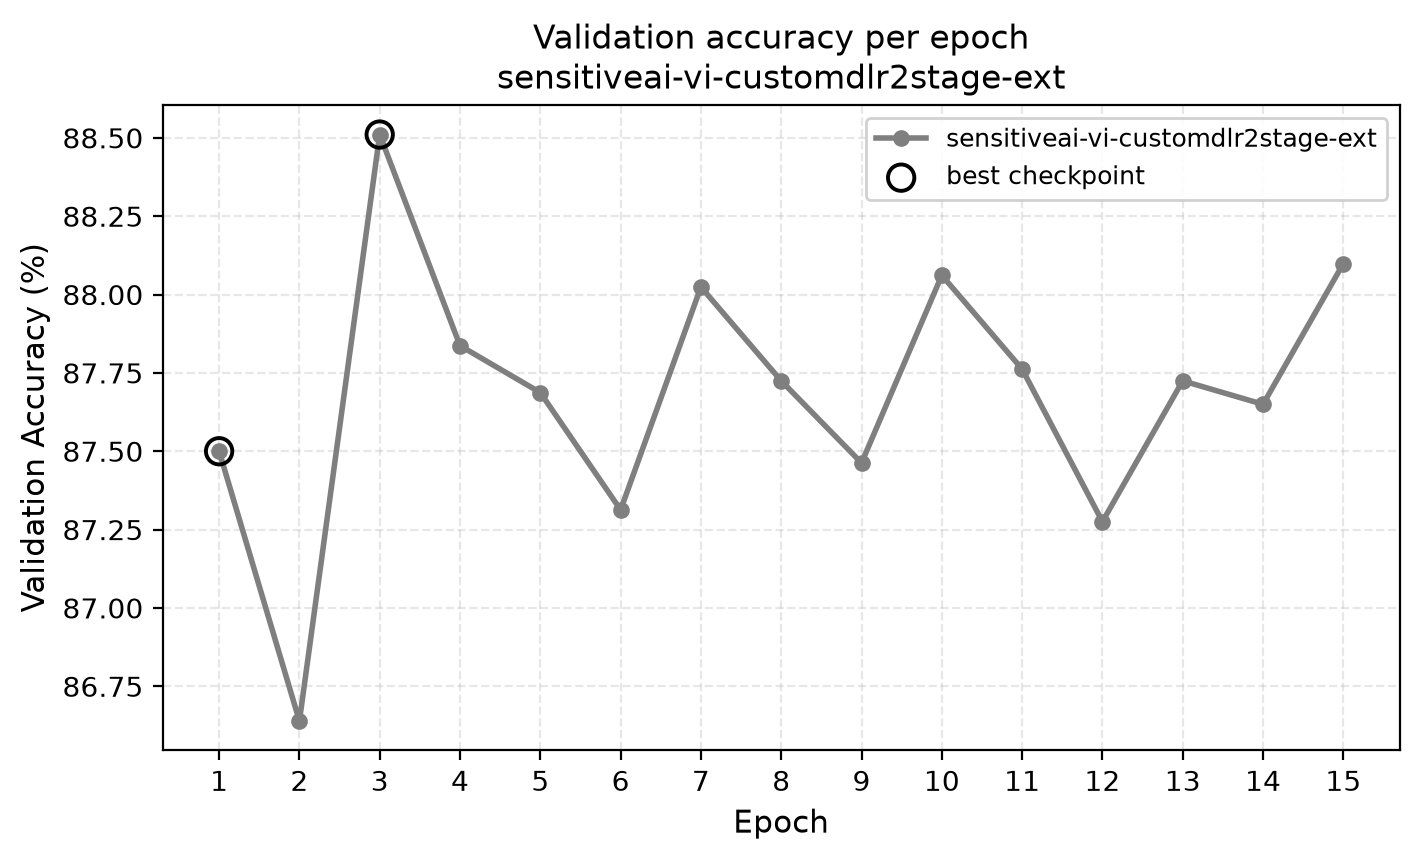
\includegraphics[width=\linewidth]{figures/per_model/M5/val_accuracy_curve.png}\caption{Validation accuracy over the training epochs.}\end{minipage}
\end{figure}


\subsection{\model{M6}}
\label{sec:supp-per-m6}
A focal-only second stage on the baseline head (class-weighted focal loss, no multi-view head).  It has the best HATE recall ($0.647$), the best HATE F1 ($0.609$) and the best macro ROC-AUC ($0.893$), but the lowest CLEAN recall ($0.922$) and the lowest accuracy ($0.863$).

\begin{figure}[htbp]
\centering
\begin{minipage}{0.74\textwidth}\centering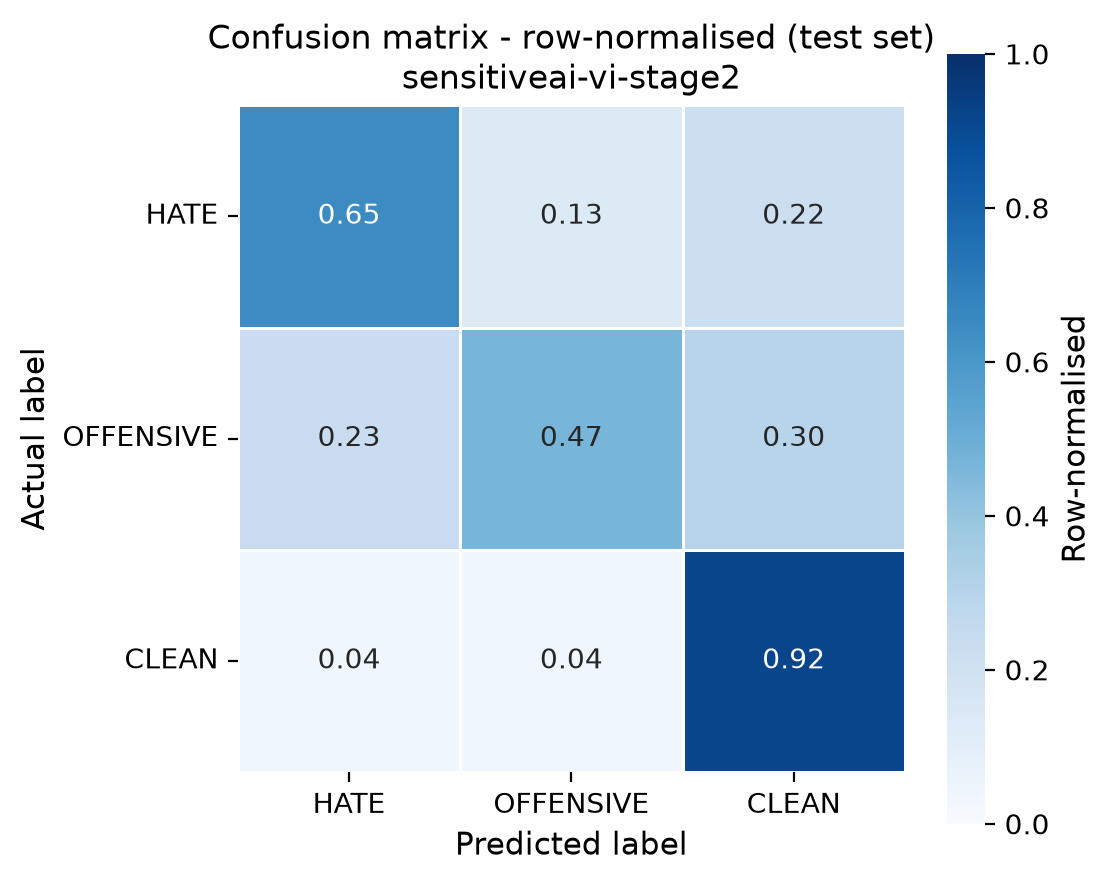
\includegraphics[width=\linewidth]{figures/per_model/M6/confusion_matrix_normalized.png}\caption{Normalised confusion matrix (rows = true, columns = predicted).}\end{minipage}
\end{figure}

\begin{figure}[htbp]
\centering
\begin{minipage}{0.74\textwidth}\centering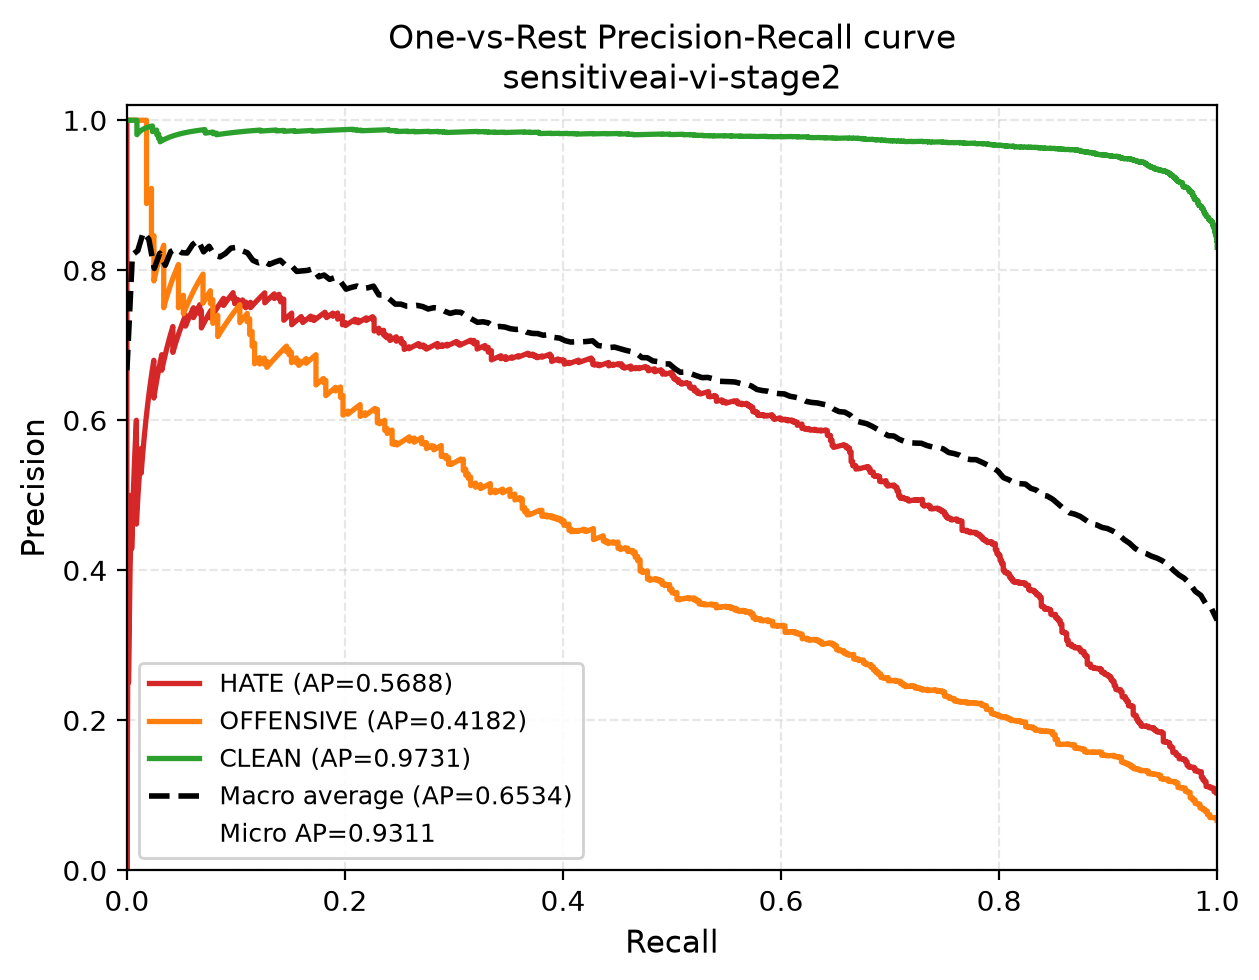
\includegraphics[width=\linewidth]{figures/per_model/M6/pr_curve.png}\caption{Precision--recall curve.}\end{minipage}
\end{figure}

\begin{figure}[htbp]
\centering
\begin{minipage}{0.74\textwidth}\centering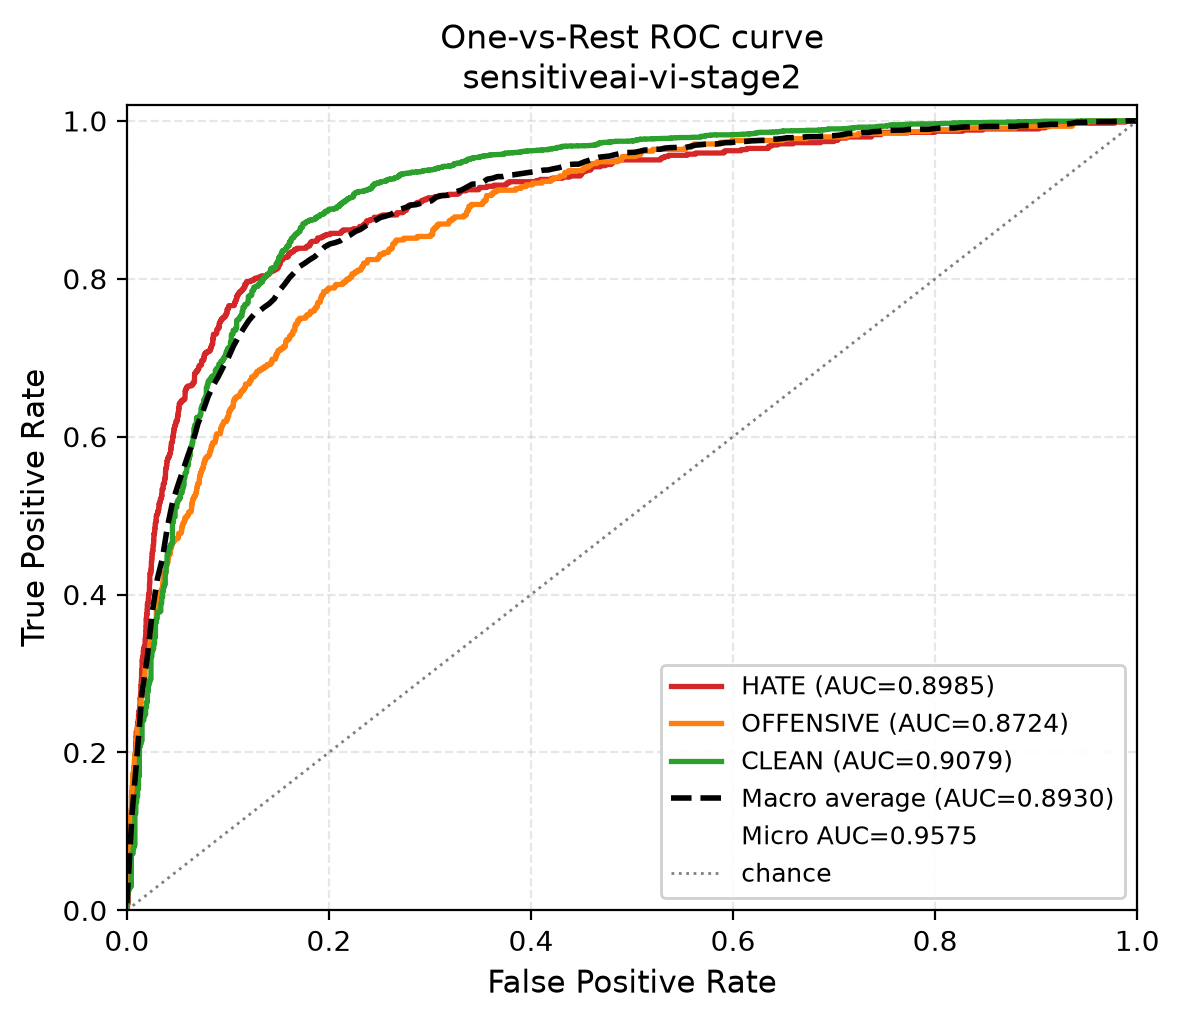
\includegraphics[width=\linewidth]{figures/per_model/M6/roc_curve.png}\caption{ROC curve.}\end{minipage}
\end{figure}

\begin{figure}[htbp]
\centering
\begin{minipage}{0.74\textwidth}\centering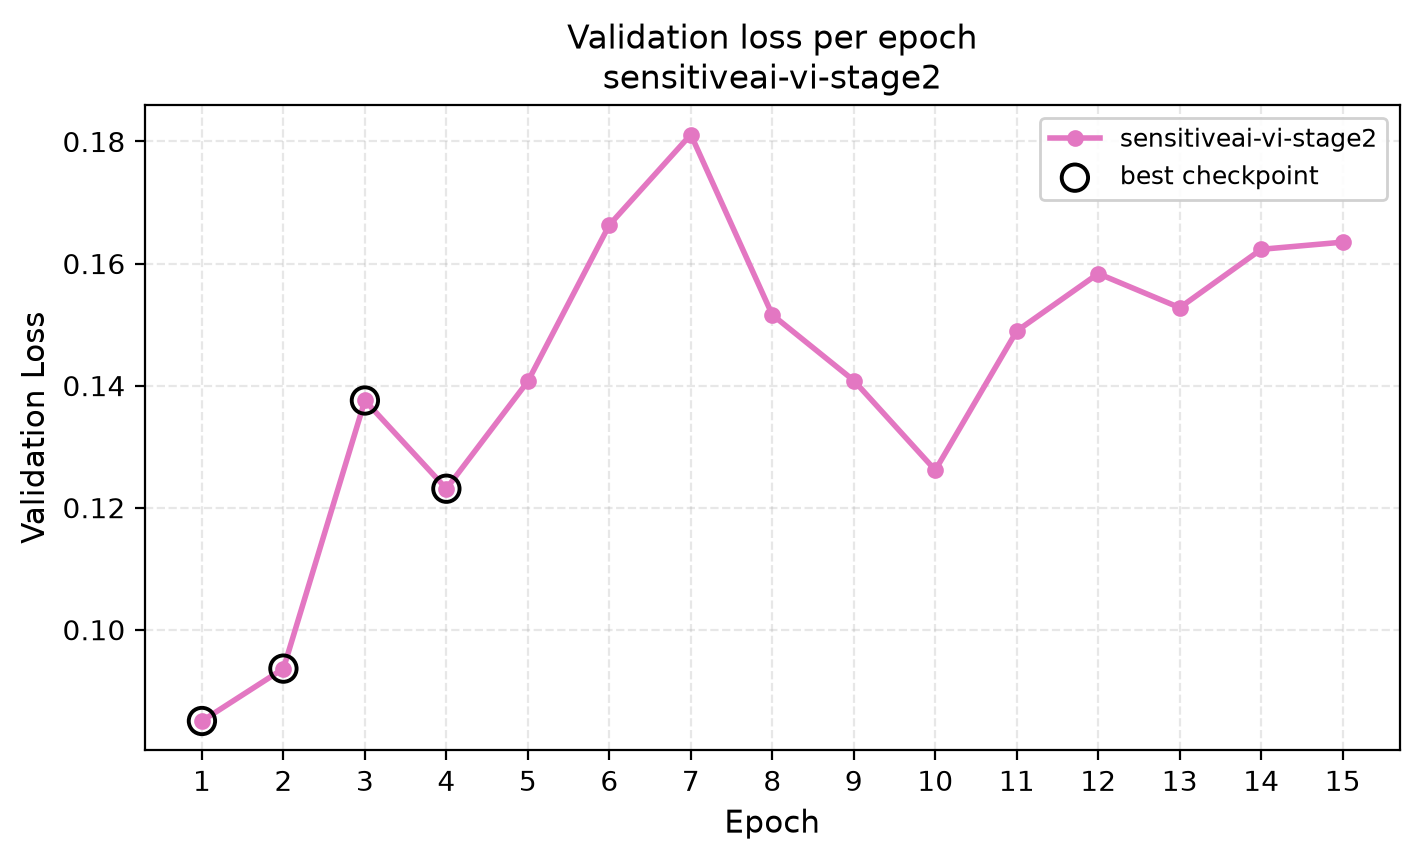
\includegraphics[width=\linewidth]{figures/per_model/M6/val_loss_curve.png}\caption{Validation loss over the training epochs.}\end{minipage}
\end{figure}

\begin{figure}[htbp]
\centering
\begin{minipage}{0.74\textwidth}\centering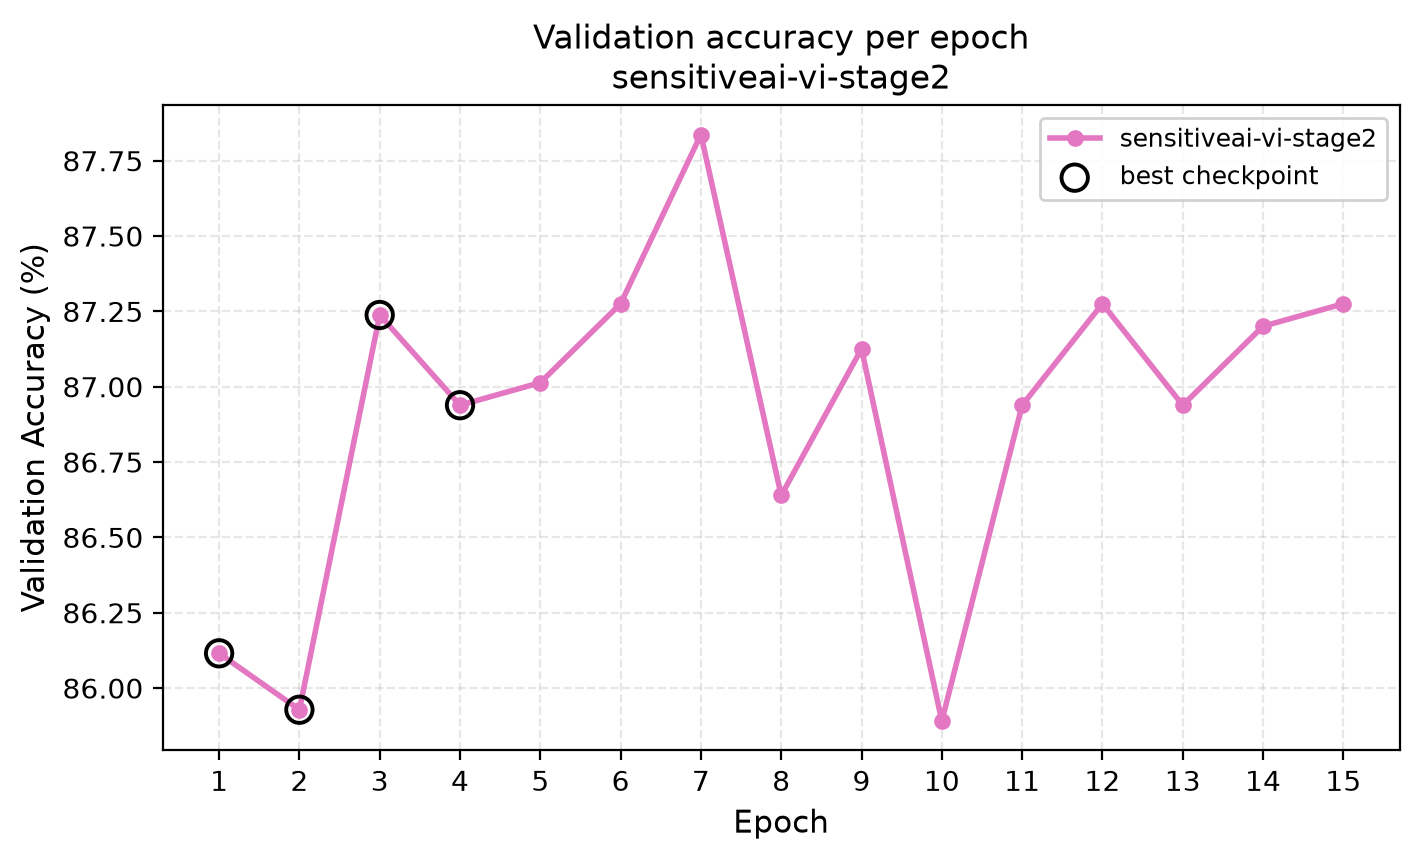
\includegraphics[width=\linewidth]{figures/per_model/M6/val_accuracy_curve.png}\caption{Validation accuracy over the training epochs.}\end{minipage}
\end{figure}



\section{Complete Pairwise Significance Matrix}
\label{sec:supp-significance}

The main paper reports a pre-specified subset of seven pairwise comparisons.
Table~\ref{tab:supp-pairs} gives the \emph{complete} matrix over all
$\binom{6}{2}=15$ pairs: the paired-bootstrap macro-F1 difference with a 95\%
confidence interval and its $p$-value, and the exact two-sided McNemar
$p$-value on accuracy, with a Holm--Bonferroni step-down correction over these
15 tests.  This complete view confirms and sharpens the main-text claim:

\begin{itemize}
  \item \textbf{Macro-F1.}  No pair is significant: every 95\% bootstrap
        interval for $\Delta$macro-F1 contains zero, consistent with the
        main-text statement that the six systems are statistically
        indistinguishable on macro-F1.
  \item \textbf{Accuracy.}  Every pair that involves \model{M6} is significant
        after Holm correction ($p_{\text{Holm}} \le 0.030$), because \model{M6}
        trades CLEAN recall for minority recall.  The main text reported this
        for the two \model{M6} pairs inside its seven-pair subset
        (\model{M3}--\model{M6} and \model{M6}--\model{M1}); the complete matrix
        shows the same effect holds for all five \model{M6} pairs.  No pair
        \emph{not} involving \model{M6} survives Holm in accuracy.
\end{itemize}

% AUTO-GENERATED by scripts/11_supplementary_analyses.py - do not edit by hand.
\begin{table}[!htbp]
\centering
\footnotesize
\setlength{\tabcolsep}{3pt}
\caption{Complete pairwise comparison of all $\binom{6}{2}=15$ system pairs. $\Delta$M-F1 is the paired-bootstrap difference ($A$ minus $B$) with a 95\% CI, $p_{\text{F1}}$ its bootstrap $p$-value; $p_{\text{acc}}$ is the exact two-sided McNemar $p$-value on accuracy.  $^{\dagger}$ marks $p<0.05$ after a Holm--Bonferroni step-down correction over these 15 tests.}
\label{tab:supp-pairs}
\begin{tabular}{lcccc}
\toprule
$A-B$ & $\Delta$M-F1 [95\% CI] & $p_{\text{F1}}$ & $p_{\text{acc}}$ (McN.) & $p_{\text{acc}}$ (Holm) \\
\midrule
M1 $-$ M2 & -0.0030 [-0.0203, +0.0144] & 0.736 & 0.370 & 1.000 \\
M1 $-$ M3 & -0.0092 [-0.0269, +0.0082] & 0.298 & 0.526 & 1.000 \\
M1 $-$ M4 & -0.0045 [-0.0215, +0.0127] & 0.594 & 0.961 & 1.000 \\
M1 $-$ M5 & +0.0009 [-0.0164, +0.0185] & 0.906 & 0.110 & 0.989 \\
M1 $-$ M6 & -0.0059 [-0.0191, +0.0071] & 0.377 & $<0.001$$^{\dagger}$ & 0.003 \\
M2 $-$ M3 & -0.0062 [-0.0186, +0.0060] & 0.328 & 0.788 & 1.000 \\
M2 $-$ M4 & -0.0015 [-0.0137, +0.0107] & 0.807 & 0.186 & 1.000 \\
M2 $-$ M5 & +0.0039 [-0.0093, +0.0174] & 0.568 & 0.385 & 1.000 \\
M2 $-$ M6 & -0.0029 [-0.0196, +0.0135] & 0.719 & $<0.001$$^{\dagger}$ & 0.002 \\
M3 $-$ M4 & +0.0047 [-0.0051, +0.0144] & 0.342 & 0.217 & 1.000 \\
M3 $-$ M5 & +0.0101 [-0.0023, +0.0228] & 0.113 & 0.217 & 1.000 \\
M3 $-$ M6 & +0.0033 [-0.0124, +0.0188] & 0.678 & $<0.001$$^{\dagger}$ & 0.002 \\
M4 $-$ M5 & +0.0054 [-0.0080, +0.0190] & 0.421 & 0.027 & 0.270 \\
M4 $-$ M6 & -0.0014 [-0.0172, +0.0139] & 0.859 & 0.003$^{\dagger}$ & 0.030 \\
M5 $-$ M6 & -0.0068 [-0.0237, +0.0098] & 0.419 & $<0.001$$^{\dagger}$ & $<0.001$ \\
\bottomrule
\end{tabular}
\end{table}


\section{Post-hoc Decision-Rule Diagnostic}
\label{sec:supp-threshold}

Because the main paper finds that a validation-searched threshold rule did not
help, it is worth asking how much a decision rule could help in the best case.
Table~\ref{tab:supp-threshold} reweights the two minority posteriors by a joint
factor $u$ and re-argmaxes, and reports the \emph{oracle} $u^{\star}$ that
maximises test macro-F1.  Within this one-parameter reweighting family the
oracle gains are tiny (at most $+0.0051$ for \model{M6}, $+0.0018$ for
\model{M1}, and exactly $0$ for \model{M3} at $u^{\star}=1$), well inside the
bootstrap confidence intervals of Table~\ref{tab:supp-pairs}.  The diagnostic
therefore bounds what \emph{this} family of decision rules can contribute, and
shows that it is not where the remaining error lies; it does not rule out
richer, class- or instance-dependent rules, and the ceiling it exposes is a
property of the frozen posteriors rather than a claim about the encoder alone.
Fig.~\ref{fig:supp-threshold} sweeps the full range of $u$.

Because $u^{\star}$ is chosen on the test set, the ``best M-F1'' column is an
upper bound and not a validated decision rule; it is reported only to bound how
much thresholding \emph{could} contribute.

% AUTO-GENERATED by scripts/11_supplementary_analyses.py - do not edit by hand.
\begin{table}[!htbp]
\centering
\footnotesize
\setlength{\tabcolsep}{4pt}
\caption{Post-hoc prior-reweighting diagnostic.  The frozen posteriors are reweighted by a joint factor $u$ on the two minority classes and re-argmaxed; $u^{\star}$ is the \emph{oracle} factor that maximises test macro-F1.  ``argmax M-F1'' is the macro-F1 of a plain argmax on the frozen posteriors; it differs from the system's headline macro-F1 only for M4, whose validation-searched thresholds ($0.01/0.5/0.64$) \emph{lowered} test macro-F1 from the argmax $0.6602$ to the reported $0.6590$.  $u^{\star}$ is chosen on the test labels and the gain is therefore an oracle upper bound over this one-parameter reweighting family, not a deployable decision rule.}
\label{tab:supp-threshold}
\begin{tabular}{lcccc}
\toprule
System & argmax M-F1 & $u^{\star}$ & best M-F1 & oracle gain \\
\midrule
M1 & 0.6545 & 0.70 & 0.6564 & +0.0018 \\
M2 & 0.6575 & 0.80 & 0.6585 & +0.0009 \\
M3 & 0.6638 & 1.00 & 0.6638 & +0.0000 \\
M4 & 0.6602 & 2.80 & 0.6616 & +0.0014 \\
M5 & 0.6536 & 3.00 & 0.6549 & +0.0012 \\
M6 & 0.6604 & 0.60 & 0.6656 & +0.0051 \\
\bottomrule
\end{tabular}
\end{table}


\begin{figure}[!htbp]
\centering
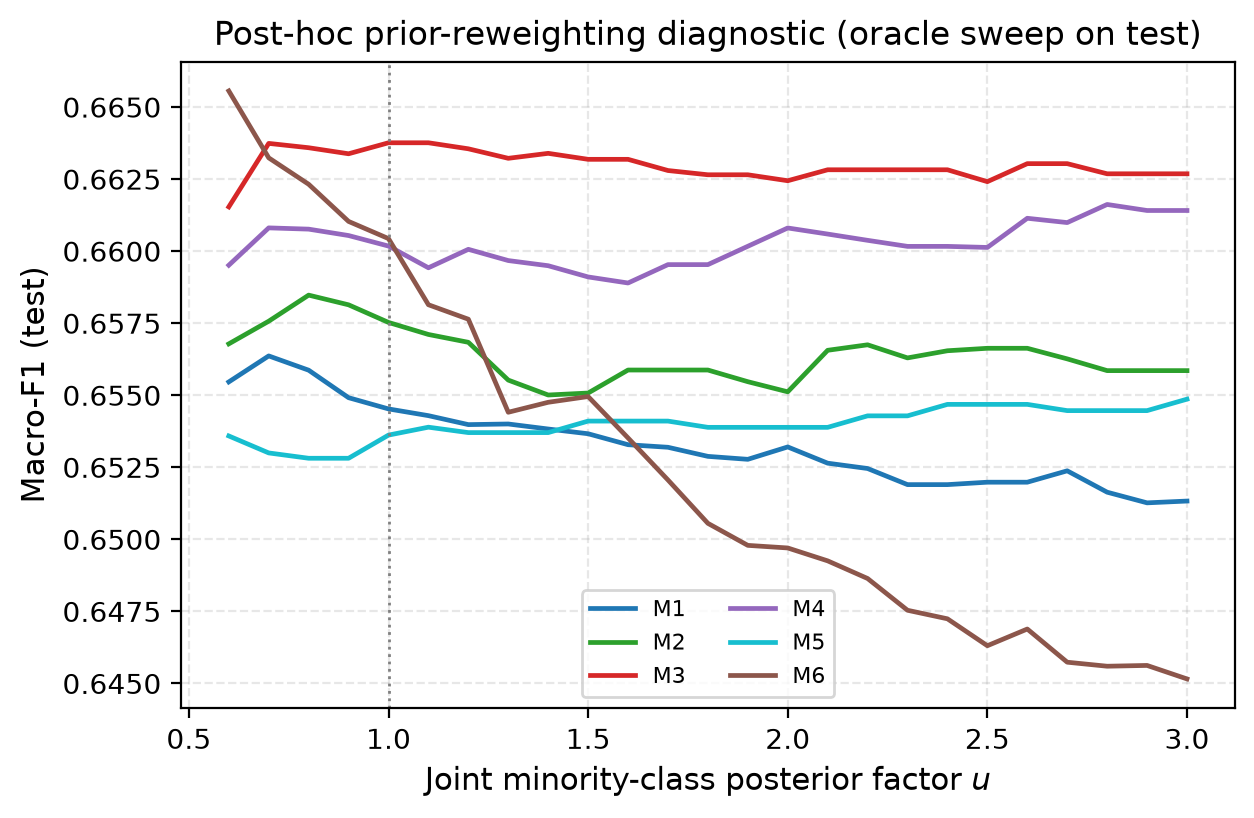
\includegraphics[width=0.7\textwidth]{threshold_sweep.png}
\caption{Test macro-F1 as a function of the minority reweighting factor $u$ for
the six systems.  The curves are flat near their maxima: no threshold change
recovers a meaningful amount of macro-F1.}
\label{fig:supp-threshold}
\end{figure}

\section{Resolved Hyperparameters and Training Cost}
\label{sec:supp-hyper}

Table~\ref{tab:supp-hyperparameters} records the resolved configuration of each
system as actually logged by the run (not as intended), and
Table~\ref{tab:supp-timing} the wall-clock cost and checkpoint selection.  The
``thr.'' column is read from each evaluated run's \texttt{metrics.json}, which is
authoritative for the test pass even where the config on disk was edited later:
\model{M1} and \model{M2} applied a plain argmax, \model{M3}--\model{M6} applied
per-class thresholds searched on validation, and only \model{M4} found
non-trivial values ($0.01/0.5/0.64$).  Three reproducibility points are worth
stating explicitly.

First, checkpoint selection is by \emph{highest validation macro-F1}
(\path{src/callbacks/monitoring.py}), not by lowest validation loss.
\model{M4} selected its \emph{first} epoch
(validation macro-F1 $0.6942$) and never beat it, so its remaining stages were
not selected---this is the mechanism behind the main-text ``curriculum did not
help'' result.  Its training log shows $19$ of $30$ planned epochs: stage~1 ran
7, stage~2 ran 6 (absolute epochs $8$--$13$) and stage~3 ran 6 (absolute epochs
$14$--$19$), and the best validation macro-F1 was achieved at absolute epoch~1,
before any of the later stages contributed.

Second, the per-class thresholds \emph{lowered} \model{M4}'s test macro-F1:
re-argmaxing the same frozen posteriors gives $0.6602$, while the reported
(thresholded) headline is $0.6590$---the searched thresholds had raised
validation macro-F1 ($0.6942 \to 0.6965$) but did not transfer to the test
split.  This is why \model{M4}'s ``argmax M-F1'' in
Table~\ref{tab:supp-threshold} is higher than its headline.

Third, \model{M5} and \model{M6} used the full fixed 15-epoch budget with the
early-stopping criterion never firing (``stopped = no'': their patience is at
least the budget), unlike \model{M1}--\model{M4}.

% AUTO-GENERATED by scripts/11_supplementary_analyses.py - do not edit by hand.
\begin{table}[!htbp]
\centering
\scriptsize
\setlength{\tabcolsep}{2pt}
\caption{Resolved per-system configuration as recorded in each run's \texttt{training\_summary.json} and \texttt{configs/*.yaml}.  ``lr'' is the stage-1 encoder rate; ``head lr'' the discriminative head rate when DLR is on.  ``thr.''\ marks the systems whose test pass applied per-class thresholds searched on validation (M3--M6, read from each run's \texttt{metrics.json}); the search returned the trivial $0.5$ for all but M4.  AdamW, weight decay 0.01, gradient clipping 1.0 and max length 256 are shared.}
\label{tab:supp-hyperparameters}
\begin{tabular}{lcccccccccc}
\toprule
System & head & stages & loss & lr & head lr & warmup & bs$\times$acc & pat. & seed & thr. \\
\midrule
M1 & standard & 1 & CE & $3.0e-05$ & $3.0e-05$ & 0.1 & 16$\times$2 & 6 & 42 & no \\
M2 & custom & 1 & CE & $3.0e-05$ & $3.0e-05$ & 0.1 & 16$\times$2 & 6 & 42 & no \\
M3 & custom & 2 & CE $\to$ focal & $2.0e-05$ & $1.0e-04$ & 0.1 & 16$\times$2 & 6 & 42 & yes \\
M4 & custom & 3 & concept $\to$ CE & $2.0e-05$ & $8.0e-05$ & 0.1 & 16$\times$2 & 6 & 42 & yes \\
M5 & custom & 1 & CE & $2.0e-05$ & $1.0e-04$ & 0.1 & 16$\times$2 & 15 & 42 & yes \\
M6 & standard & 1 & focal & $1.0e-05$ & $1.0e-05$ & 0.05 & 16$\times$2 & 20 & 42 & yes \\
\bottomrule
\end{tabular}
\end{table}

% AUTO-GENERATED by scripts/11_supplementary_analyses.py - do not edit by hand.
\begin{table}[!htbp]
\centering
\footnotesize
\setlength{\tabcolsep}{4pt}
\caption{Wall-clock cost and checkpoint selection per system.  ``best ep.'' is the epoch whose validation macro-F1 was frozen for the test pass and ``stopped'' whether early stopping fired before the planned epoch budget.}
\label{tab:supp-timing}
\begin{tabular}{lccccc}
\toprule
System & epochs & planned & best ep. & stopped & wall clock \\
\midrule
M1 & 15 & 30 & 9 & yes & 02:50:03 \\
M2 & 20 & 30 & 14 & yes & 03:50:56 \\
M3 & 21 & 30 & 15 & yes & 03:56:46 \\
M4 & 19 & 30 & 1 & yes & 03:38:41 \\
M5 & 15 & 15 & 3 & no & 02:48:28 \\
M6 & 15 & 15 & 4 & no & 02:59:21 \\
\bottomrule
\end{tabular}
\end{table}


\section{Complementary Experiments}
\label{sec:supp-complementary}

Two further experiments are provided as runnable scripts but are \emph{not}
part of the main results, because ensuring they were meaningful (rather than
noise) would require compute beyond a single training session.

\begin{itemize}
  \item \textbf{Seed variance} (\path{scripts/09_seed_variance.py})
        re-trains each of the six recipes under five seeds (30 runs) so that a
        seed-variance floor can be placed under the 0.654--0.664 macro-F1 band.
        On the available single-GPU budget this is roughly 60\,h of training
        and was out of scope; the script is included so the experiment can be
        reproduced, and the main text is careful not to \emph{claim} a
        seed-robust ordering.
  \item \textbf{Monolingual encoders}
        (\path{scripts/10_train_monolingual_baselines.py}), which trains
        PhoBERT (\texttt{vinai/phobert-base-v2}) and ViSoBERT
        (\texttt{uitnlp/visobert}) under the same recipe as the baseline, to
        test whether the multilingual backbone is actually doing work.  This is
        a separate comparison and is deliberately kept out of the six-system
        ablation so as not to confound the optimisation-recipe study.
\end{itemize}

\section{Reproduction}
\label{sec:supp-reproduce}

All tables and figures in this supplement are generated from the frozen
artefacts by
\begin{center}
\texttt{python scripts/11\_supplementary\_analyses.py}
\end{center}
which reads the per-system \path{test_predictions.csv}, \path{metrics.json} and
\path{training_summary.json} under \path{outputs/evaluation/per_model/} and
writes \path{papers/supplementary/tables/*.tex},
\path{papers/supplementary/figures/*.png} and a machine-readable summary at
\path{outputs/evaluation/analysis/supplementary_report.md} and
\path{supplementary_summary.json}.  The frozen run snapshot
\path{outputs/evaluation/per_model/<system>/config.yaml} is treated as
authoritative for each evaluated system: the top-level \path{configs/*.yaml} may
have been edited after a run (this is the case for \model{M6}, whose on-disk
config now shows the threshold search disabled although the evaluated run
enabled it).  The bootstrap uses 10{,}000 resamples with a fixed seed, so the
intervals are
deterministic given the frozen predictions.  This document is then compiled
with \texttt{pdflatex} + \texttt{bibtex} in \texttt{papers/supplementary/}.

\FloatBarrier
\bibliographystyle{splncs04}
{\let\small\scriptsize\bibliography{references}}

\end{document}
